%%%%%%%%%%%%%%%%%%%%%%%%%%%%%%%%%%%%%%%%%
% Masters/Doctoral Thesis
% LaTeX Template
% Version 2.5 (27/8/17)
%
% This template was downloaded from:
% http://www.LaTeXTemplates.com/template/masters-doctoral-thesis
%
% Version 2.x major modifications by:
% Vel (vel@latextemplates.com)
%
% This template is based on a template by:
% Steve Gunn (http://users.ecs.soton.ac.uk/srg/softwaretools/document/templates/)
% Sunil Patel (http://www.sunilpatel.co.uk/thesis-template/)
%
% Template license:
% CC BY-NC-SA 3.0 (http://creativecommons.org/licenses/by-nc-sa/3.0/)
%
%%%%%%%%%%%%%%%%%%%%%%%%%%%%%%%%%%%%%%%%%

%----------------------------------------------------------------------------------------
%	PACKAGES AND OTHER DOCUMENT CONFIGURATIONS
%----------------------------------------------------------------------------------------

\documentclass[
	12pt, % The default document font size, options: 10pt, 11pt, 12pt
	% oneside, % Two side (alternating margins) for binding by default, uncomment to switch to one side
	english, % ngerman for German
	singlespacing, % Single line spacing, alternatives: onehalfspacing or doublespacing
	%draft, % Uncomment to enable draft mode (no pictures, no links, overfull hboxes indicated)
	%nolistspacing, % If the document is onehalfspacing or doublespacing, uncomment this to set spacing in lists to single
	liststotoc, % Uncomment to add the list of figures/tables/etc to the table of contents
	toctotoc, % Uncomment to add the main table of contents to the table of contents
	parskip, % Uncomment to add space between paragraphs
	%nohyperref, % Uncomment to not load the hyperref package
	headsepline, % Uncomment to get a line under the header
	% chapterinoneline, % Uncomment to place the chapter title next to the number on one line
	% consistentlayout, % Uncomment to change the layout of the declaration, abstract and acknowledgements pages to match the default layout
]{MastersDoctoralThesis} % The class file specifying the document structure

\usepackage[utf8]{inputenc} % Required for inputting international characters
\usepackage[T1]{fontenc} % Output font encoding for international characters
% \usepackage[british]{babel}

\usepackage{mathpazo} % Use the Palatino font by default

\usepackage[backend=bibtex,style=numeric,natbib=true,sorting=none]{biblatex} % Use the bibtex backend with the numeric citation style
% \usepackage[backend=bibtex,style=numeric,natbib=true]{biblatex} % Use the bibtex backend with the numeric citation style

% \addbibresource{example.bib} % The filename of the bibliography
\addbibresource{References.bib} % The filename of the bibliography

\usepackage[autostyle=true]{csquotes} % Required to generate language-dependent quotes in the bibliography

\usepackage[section]{placeins}
\usepackage{float}

\makeatletter

% \AtBeginDocument{
% 	\expandafter\renewcommand\expandafter\subsection\expandafter{
% 		\expandafter\@fb@secFB\subsection
% 	}
% }

\makeatother

\addtocontents{loa}{\def\string\figurename{Algorithm}}

\usepackage{comment}
\usepackage{algorithm}
\usepackage[noend]{algpseudocode}
\usepackage{hyperref}

\usepackage{graphicx}
\def\infinity{\rotatebox{90}{8}}
\usepackage{amsmath}

%----------------------------------------------------------------------------------------
%	MARGIN SETTINGS
%----------------------------------------------------------------------------------------

\geometry{
	paper=a4paper, % Change to letterpaper for US letter
	inner=2.5cm, % Inner margin
	outer=3.8cm, % Outer margin
	bindingoffset=.5cm, % Binding offset
	top=1.5cm, % Top margin
	bottom=1.5cm, % Bottom margin
	%showframe, % Uncomment to show how the type block is set on the page
}

%----------------------------------------------------------------------------------------
%	THESIS INFORMATION
%----------------------------------------------------------------------------------------

\thesistitle{Design and Implementation of AlexNet Deep Learning Network using Reconfigurable Logic} % Your thesis title, this is used in the title and abstract, print it elsewhere with \ttitle
\supervisor{Pr. Apostolos \textsc{Dollas}} % Your supervisor's name, this is used in the title page, print it elsewhere with \supname
\examiner{} % Your examiner's name, this is not currently used anywhere in the template, print it elsewhere with \examname
\degree{Electrical and Computer Engineer} % Your degree name, this is used in the title page and abstract, print it elsewhere with \degreename
\author{Tzanis \textsc{Fotakis}} % Your name, this is used in the title page and abstract, print it elsewhere with \authorname
\addresses{} % Your address, this is not currently used anywhere in the template, print it elsewhere with \addressname

\subject{Electrical and Computer Engineering} % Your subject area, this is not currently used anywhere in the template, print it elsewhere with \subjectname
\keywords{Diploma Thesis} % Keywords for your thesis, this is not currently used anywhere in the template, print it elsewhere with \keywordnames
\university{\href{https://www.tuc.gr/}{Technical University of Crete}} % Your university's name and URL, this is used in the title page and abstract, print it elsewhere with \univname
\department{\href{https://www.ece.tuc.gr/}{School of Electrical and Computer Engineering}} % Your department's name and URL, this is used in the title page and abstract, print it elsewhere with \deptname
\group{\href{https://www.mhl.tuc.gr/}{Microprocessor and Hardware Laboratory}} % Your research group's name and URL, this is used in the title page, print it elsewhere with \groupname
\faculty{
		% \href{http://faculty.university.com}{Faculty Name}
} % Your faculty's name and URL, this is used in the title page and abstract, print it elsewhere with \facname

\AtBeginDocument{
	\hypersetup{pdftitle=\ttitle} % Set the PDF's title to your title
	\hypersetup{pdfauthor=\authorname} % Set the PDF's author to your name
	\hypersetup{pdfkeywords=\keywordnames} % Set the PDF's keywords to your keywords
}

\begin{document}

\frontmatter % Use roman page numbering style (i, ii, iii, iv...) for the pre-content pages

\pagestyle{plain} % Default to the plain heading style until the thesis style is called for the body content

%----------------------------------------------------------------------------------------
%	TITLE PAGE
%----------------------------------------------------------------------------------------

\begin{titlepage}
	\begin{center}

		\vspace*{.06\textheight}
		{\scshape\LARGE \univname\par}\vspace{1.5cm} % University name
		\textsc{\Large Diploma Thesis}\\[0.5cm] % Thesis type

		\HRule \\[0.4cm] % Horizontal line
		{\huge \bfseries \ttitle\par}\vspace{0.4cm} % Thesis title
		\HRule \\[1.5cm] % Horizontal line

		\begin{minipage}[t]{0.4\textwidth}
			\begin{flushleft} \large
				\emph{Author:}\\
				\href{https://www.linkedin.com/in/fotakistzanis/}{\authorname} % Author name - remove the \href bracket to remove the link
			\end{flushleft}
		\end{minipage}
		\begin{minipage}[t]{0.5\textwidth}
			\begin{flushright} \large
				\emph{Thesis Committee:} \\
				\href{https://www.ece.tuc.gr/index.php?id=4531&tx_tuclabspersonnel_list%5Bperson%5D=289&tx_tuclabspersonnel_list%5Baction%5D=person&tx_tuclabspersonnel_list%5Bcontroller%5D=List}{Prof. Apostolos \textsc{Dollas}}\\ % Supervisor name - remove the \href bracket to remove the link
				\href{https://www.ece.tuc.gr/index.php?id=4531&tx_tuclabspersonnel_list%5Bperson%5D=313&tx_tuclabspersonnel_list%5Baction%5D=person&tx_tuclabspersonnel_list%5Bcontroller%5D=List}{Prof. Michail \textsc{Lagoudakis}}\\
				\href{https://www.linkedin.com/in/christos-kozanitis-a3b173a8/}{Dr. Christos \textsc{Kozanitis}}
			\end{flushright}
		\end{minipage}\\[0.2cm]

		
\includegraphics[scale=0.21]{Images/TUC_logo.png} % University/department logo - uncomment to place it
		\\[0.5cm]

		\vfill

		\large \textit{A thesis submitted in fulfillment of the requirements\\ for the diploma of \degreename}\\[0.3cm] % University requirement text
		\textit{in the}\\[0.4cm]
		\deptname\\\groupname\\[2cm] % Research group name and department name

		\vfill

		{\large \today}\\[4cm] % Date
		%\includegraphics{Logo} % University/department logo - uncomment to place it

		\vfill
	\end{center}
\end{titlepage}

%----------------------------------------------------------------------------------------
%	DECLARATION PAGE
%----------------------------------------------------------------------------------------

\begin{comment}
\begin{declaration}
	\addchaptertocentry{\authorshipname} % Add the declaration to the table of contents
	\noindent I, \authorname, declare that this thesis titled, \enquote{\ttitle} and the work presented in it are my own. I confirm that:

	\begin{itemize}
		\item This work was done wholly or mainly while in candidature for a research degree at this University.
		\item Where any part of this thesis has previously been submitted for a degree or any other qualification at this University or any other institution, this has been clearly stated.
		\item Where I have consulted the published work of others, this is always clearly attributed.
		\item Where I have quoted from the work of others, the source is always given. With the exception of such quotations, this thesis is entirely my own work.
		\item I have acknowledged all main sources of help.
		\item Where the thesis is based on work done by myself jointly with others, I have made clear exactly what was done by others and what I have contributed myself.\\
	\end{itemize}

	\noindent Signed:\\
	\rule[0.5em]{25em}{0.5pt} % This prints a line for the signature

	\noindent Date:\\
	\rule[0.5em]{25em}{0.5pt} % This prints a line to write the date
\end{declaration}

\cleardoublepage
\end{comment}

%----------------------------------------------------------------------------------------
%	QUOTATION PAGE
%----------------------------------------------------------------------------------------

\begin{comment}
\vspace*{0.2\textheight}

\noindent\enquote{\itshape Thanks to my solid academic training, today I can write hundreds of words on virtually any topic without possessing a shred of information, which is how I got a good job in journalism.}\bigbreak

\hfill Dave Barry
\end{comment}

%----------------------------------------------------------------------------------------
%	ABSTRACT PAGE
%----------------------------------------------------------------------------------------

\begin{abstract}
	\addchaptertocentry{\abstractname} % Add the abstract to the table of contents
	% Todo: Add Abstract
	The Thesis Abstract is written here (and usually kept to just this page). The page is kept centered vertically so can expand into the blank space above the title too\ldots
\end{abstract}

%----------------------------------------------------------------------------------------
%	ACKNOWLEDGEMENTS
%----------------------------------------------------------------------------------------

\begin{acknowledgements}
	\addchaptertocentry{\acknowledgementname} % Add the acknowledgements to the table of contents
	% Todo: Add Acknowledgements
	The acknowledgments and the people to thank go here, don't forget to include your project advisor\ldots
\end{acknowledgements}

%----------------------------------------------------------------------------------------
%	LIST OF CONTENTS/FIGURES/TABLES PAGES
%----------------------------------------------------------------------------------------

\tableofcontents % Prints the main table of contents

\listoffigures % Prints the list of figures

\listoftables % Prints the list of tables

\listofalgorithms % Prints the list of algorithms
\addcontentsline{toc}{chapter}{List of Algorithms}

%----------------------------------------------------------------------------------------
%	ABBREVIATIONS
%----------------------------------------------------------------------------------------

% spell-checker: disable
\begin{abbreviations}{ll} % Include a list of abbreviations (a table of two columns)

	\textbf{AI}		& \textbf{A}rtificial \textbf{I}ntelligence\\
	\textbf{ALU}	& \textbf{A}rithmetic \textbf{L}ogic \textbf{U}nit\\
	\textbf{ANN}	& \textbf{A}rtificial \textbf{N}eural \textbf{N}etwork\\
	\textbf{ASIC}	& \textbf{A}pplication \textbf{S}pecific \textbf{I}ntegrated \textbf{C}ircuit\\
	\textbf{BRAM}	& \textbf{B}lock \textbf{R}andom \textbf{A}ccess \textbf{M}emory\\
	\textbf{CNN}	& \textbf{C}onvolutional \textbf{N}eural \textbf{N}etwork\\
	\textbf{CPU}	& \textbf{C}entral \textbf{P}rocessor \textbf{U}nit\\
	\textbf{CS}		& \textbf{C}omputer \textbf{S}cience\\
	\textbf{CUDA}	& \textbf{C}ompute \textbf{U}nified \textbf{D}evice \textbf{A}rchitecture\\
	\textbf{cuDNN}	& \textbf{C}UDA \textbf{D}eep \textbf{N}eural \textbf{N}etwork library\\
	\textbf{DDR4}	& \textbf{D}ouble \textbf{D}ata \textbf{R}ate type texbf{4} memory\\
	\textbf{DRAM}	& \textbf{D}ynamic \textbf{R}andom \textbf{A}ccess \textbf{M}emory\\
	\textbf{DNN}	& \textbf{D}eep \textbf{N}eural \textbf{N}etwork\\
	\textbf{DPU}	& \textbf{D}eep Learning \textbf{P}rocessing \textbf{U}nit\\
	\textbf{DSP}	& \textbf{D}igital \textbf{S}ignal \textbf{P}rocessor\\
	\textbf{FC}		& \textbf{F}ully \textbf{C}onnected\\
	\textbf{FF}		& \textbf{F}lip \textbf{F}lops\\
	\textbf{FPGA}	& \textbf{F}ield \textbf{P}rogrammable \textbf{G}ate \textbf{A}rray\\
	\textbf{FORTH}	& \textbf{F}undation of \textbf{R}esearch and \textbf{T}echnology \textbf{H}ellas\\
	\textbf{GDDR6}	& \textbf{G}raphics \textbf{D}ouble \textbf{D}ata \textbf{R}ate type \textbf{6} memory\\
	\textbf{GPU}	& \textbf{G}raphic \textbf{P}rocessor \textbf{U}nit\\
	\textbf{HBM}	& \textbf{H}igh \textbf{B}andwidth \textbf{M}emory\\
	\textbf{HLS}	& \textbf{H}igh \textbf{L}evel \textbf{S}ynthesis\\
	\textbf{HPC}	& \textbf{H}ight \textbf{P}erformance \textbf{C}omputing\\
	\textbf{ILSVRC}	& \textbf{I}mageNet \textbf{L}arge \textbf{S}cale \textbf{V}isual \textbf{R}ecognition \textbf{C}hallenge\\
	\textbf{LUT}	& \textbf{L}ook \textbf{U}p \textbf{T}able\\
	\textbf{ML}		& \textbf{M}achine \textbf{L}earning\\
	\textbf{MLP}	& \textbf{M}ulti-\textbf{L}ayer \textbf{P}erceptron\\
	\textbf{MPSoC}	& \textbf{M}ulti \textbf{P}rocessor \textbf{S}ystem \textbf{o}n \textbf{C}hip\\
	\textbf{MXU}	& \textbf{M}atrix Mutliplier \textbf{U}nit\\
	\textbf{PE}		& \textbf{P}rocessing \textbf{E}lement\\
	\textbf{PL}		& \textbf{P}rogrammable \textbf{L}ogic\\
	\textbf{PS}		& \textbf{P}rocessing \textbf{S}ystem\\
	\textbf{QFDB}	& \textbf{Q}uad \textbf{F}PGA \textbf{D}aughter \textbf{B}oard\\
	\textbf{RAM}	& \textbf{R}andom \textbf{A}ccess \textbf{M}emory\\
	\textbf{ReLU}	& \textbf{R}ectified \textbf{L}inear \textbf{U}nit\\
	\textbf{SDK}	& \textbf{S}oftware \textbf{D}evelopment \textbf{K}it\\
	\textbf{SIMD}	& \textbf{S}ingle \textbf{I}nstruction \textbf{M}ultiple \textbf{D}ata\\
	\textbf{SM}		& \textbf{S}treaming \textbf{M}ultiprocessor\\
	\textbf{SLC}	& \textbf{S}econd \textbf{L}evel \textbf{C}odebook\\
	\textbf{SSE}	& \textbf{S}treaming \textbf{S}IMD \textbf{E}xtensions\\
	\textbf{SSD}	& \textbf{S}olid \textbf{S}tate \textbf{D}rive\\
	\textbf{TDP}	& \textbf{T}hermal \textbf{D}esign \textbf{P}ower\\
	\textbf{TPU}	& \textbf{T}ensor \textbf{P}rocessor \textbf{U}nit\\
	\textbf{URAM}	& \textbf{U}ltra \textbf{R}andom \textbf{A}ccess \textbf{M}emory\\
	\textbf{USD}	& \textbf{U}nited \textbf{S}tates \textbf{D}ollar\\

\end{abbreviations}
% spell-checker: enable

%----------------------------------------------------------------------------------------
%	PHYSICAL CONSTANTS/OTHER DEFINITIONS
%----------------------------------------------------------------------------------------

\begin{comment}
\begin{constants}{lr@{${}={}$}l} % The list of physical constants is a three column table

	% The \SI{}{} command is provided by the siunitx package, see its documentation for instructions on how to use it

	Speed of Light & $c_{0}$ & \SI{2.99792458e8}{\meter\per\second} (exact)\\
	%Constant Name & $Symbol$ & $Constant Value$ with units\\

\end{constants}
\end{comment}

%----------------------------------------------------------------------------------------
%	SYMBOLS
%----------------------------------------------------------------------------------------

\begin{comment}
\begin{symbols}{lll} % Include a list of Symbols (a three column table)

	$a$ & distance & \si{\meter} \\
	$P$ & power & \si{\watt} (\si{\joule\per\second}) \\
	%Symbol & Name & Unit \\

	\addlinespace % Gap to separate the Roman symbols from the Greek

	$\omega$ & angular frequency & \si{\radian} \\

\end{symbols}
\end{comment}

%----------------------------------------------------------------------------------------
%	DEDICATION
%----------------------------------------------------------------------------------------

\dedicatory{Dedicated to my family and friends\ldots}

%----------------------------------------------------------------------------------------
%	THESIS CONTENT - CHAPTERS
%----------------------------------------------------------------------------------------

% Include the chapters of the thesis as separate files from the Chapters folder
% Uncomment the lines as you write the chapters
\pagestyle{thesis} % Return the page headers back to the "thesis" style
% % Chapter 1

\chapter{Chapter Title Here} % Main chapter title

\label{Chapter1} % For referencing the chapter elsewhere, use \ref{Chapter1}

%----------------------------------------------------------------------------------------

% Define some commands to keep the formatting separated from the content
\newcommand{\keyword}[1]{\textbf{#1}}
\newcommand{\tabhead}[1]{\textbf{#1}}
\newcommand{\code}[1]{\texttt{#1}}
\newcommand{\file}[1]{\texttt{\bfseries#1}}
\newcommand{\option}[1]{\texttt{\itshape#1}}

%----------------------------------------------------------------------------------------

\section{Welcome and Thank You}
Welcome to this \LaTeX{} Thesis Template, a beautiful and easy to use template for writing a thesis using the \LaTeX{} typesetting system.

If you are writing a thesis (or will be in the future) and its subject is technical or mathematical (though it doesn't have to be), then creating it in \LaTeX{} is highly recommended as a way to make sure you can just get down to the essential writing without having to worry over formatting or wasting time arguing with your word processor.

\LaTeX{} is easily able to professionally typeset documents that run to hundreds or thousands of pages long. With simple mark-up commands, it automatically sets out the table of contents, margins, page headers and footers and keeps the formatting consistent and beautiful. One of its main strengths is the way it can easily typeset mathematics, even \emph{heavy} mathematics. Even if those equations are the most horribly twisted and most difficult mathematical problems that can only be solved on a super-computer, you can at least count on \LaTeX{} to make them look stunning.

%----------------------------------------------------------------------------------------

\section{Learning \LaTeX{}}

\LaTeX{} is not a \textsc{wysiwyg} (What You See is What You Get) program, unlike word processors such as Microsoft Word or Apple's Pages. Instead, a document written for \LaTeX{} is actually a simple, plain text file that contains \emph{no formatting}. You tell \LaTeX{} how you want the formatting in the finished document by writing in simple commands amongst the text, for example, if I want to use \emph{italic text for emphasis}, I write the \verb|\emph{text}| command and put the text I want in italics in between the curly braces. This means that \LaTeX{} is a \enquote{mark-up} language, very much like HTML.

\subsection{A (not so short) Introduction to \LaTeX{}}

If you are new to \LaTeX{}, there is a very good eBook -- freely available online as a PDF file -- called, \enquote{The Not So Short Introduction to \LaTeX{}}. The book's title is typically shortened to just \emph{lshort}. You can download the latest version (as it is occasionally updated) from here:
\url{http://www.ctan.org/tex-archive/info/lshort/english/lshort.pdf}

It is also available in several other languages. Find yours from the list on this page: \url{http://www.ctan.org/tex-archive/info/lshort/}

It is recommended to take a little time out to learn how to use \LaTeX{} by creating several, small `test' documents, or having a close look at several templates on:\\
\url{http://www.LaTeXTemplates.com}\\
Making the effort now means you're not stuck learning the system when what you \emph{really} need to be doing is writing your thesis.

\subsection{A Short Math Guide for \LaTeX{}}

If you are writing a technical or mathematical thesis, then you may want to read the document by the AMS (American Mathematical Society) called, \enquote{A Short Math Guide for \LaTeX{}}. It can be found online here:
\url{http://www.ams.org/tex/amslatex.html}
under the \enquote{Additional Documentation} section towards the bottom of the page.

\subsection{Common \LaTeX{} Math Symbols}
There are a multitude of mathematical symbols available for \LaTeX{} and it would take a great effort to learn the commands for them all. The most common ones you are likely to use are shown on this page:
\url{http://www.sunilpatel.co.uk/latex-type/latex-math-symbols/}

You can use this page as a reference or crib sheet, the symbols are rendered as large, high quality images so you can quickly find the \LaTeX{} command for the symbol you need.

\subsection{\LaTeX{} on a Mac}

The \LaTeX{} distribution is available for many systems including Windows, Linux and Mac OS X. The package for OS X is called MacTeX and it contains all the applications you need -- bundled together and pre-customized -- for a fully working \LaTeX{} environment and work flow.

MacTeX includes a custom dedicated \LaTeX{} editor called TeXShop for writing your `\file{.tex}' files and BibDesk: a program to manage your references and create your bibliography section just as easily as managing songs and creating playlists in iTunes.

%----------------------------------------------------------------------------------------

\section{Getting Started with this Template}

If you are familiar with \LaTeX{}, then you should explore the directory structure of the template and then proceed to place your own information into the \emph{THESIS INFORMATION} block of the \file{main.tex} file. You can then modify the rest of this file to your unique specifications based on your degree/university. Section \ref{FillingFile} on page \pageref{FillingFile} will help you do this. Make sure you also read section \ref{ThesisConventions} about thesis conventions to get the most out of this template.

If you are new to \LaTeX{} it is recommended that you carry on reading through the rest of the information in this document.

Before you begin using this template you should ensure that its style complies with the thesis style guidelines imposed by your institution. In most cases this template style and layout will be suitable. If it is not, it may only require a small change to bring the template in line with your institution's recommendations. These modifications will need to be done on the \file{MastersDoctoralThesis.cls} file.

\subsection{About this Template}

This \LaTeX{} Thesis Template is originally based and created around a \LaTeX{} style file created by Steve R.\ Gunn from the University of Southampton (UK), department of Electronics and Computer Science. You can find his original thesis style file at his site, here:
\url{http://www.ecs.soton.ac.uk/~srg/softwaretools/document/templates/}

Steve's \file{ecsthesis.cls} was then taken by Sunil Patel who modified it by creating a skeleton framework and folder structure to place the thesis files in. The resulting template can be found on Sunil's site here:
\url{http://www.sunilpatel.co.uk/thesis-template}

Sunil's template was made available through \url{http://www.LaTeXTemplates.com} where it was modified many times based on user requests and questions. Version 2.0 and onwards of this template represents a major modification to Sunil's template and is, in fact, hardly recognisable. The work to make version 2.0 possible was carried out by \href{mailto:vel@latextemplates.com}{Vel} and Johannes Böttcher.

%----------------------------------------------------------------------------------------

\section{What this Template Includes}

\subsection{Folders}

This template comes as a single zip file that expands out to several files and folders. The folder names are mostly self-explanatory:

\keyword{Appendices} -- this is the folder where you put the appendices. Each appendix should go into its own separate \file{.tex} file. An example and template are included in the directory.

\keyword{Chapters} -- this is the folder where you put the thesis chapters. A thesis usually has about six chapters, though there is no hard rule on this. Each chapter should go in its own separate \file{.tex} file and they can be split as:
\begin{itemize}
	\item Chapter 1: Introduction to the thesis topic
	\item Chapter 2: Background information and theory
	\item Chapter 3: (Laboratory) experimental setup
	\item Chapter 4: Details of experiment 1
	\item Chapter 5: Details of experiment 2
	\item Chapter 6: Discussion of the experimental results
	\item Chapter 7: Conclusion and future directions
\end{itemize}
This chapter layout is specialised for the experimental sciences, your discipline may be different.

\keyword{Figures} -- this folder contains all figures for the thesis. These are the final images that will go into the thesis document.

\subsection{Files}

Included are also several files, most of them are plain text and you can see their contents in a text editor. After initial compilation, you will see that more auxiliary files are created by \LaTeX{} or BibTeX and which you don't need to delete or worry about:

\keyword{example.bib} -- this is an important file that contains all the bibliographic information and references that you will be citing in the thesis for use with BibTeX. You can write it manually, but there are reference manager programs available that will create and manage it for you. Bibliographies in \LaTeX{} are a large subject and you may need to read about BibTeX before starting with this. Many modern reference managers will allow you to export your references in BibTeX format which greatly eases the amount of work you have to do.

\keyword{MastersDoctoralThesis.cls} -- this is an important file. It is the class file that tells \LaTeX{} how to format the thesis.

\keyword{main.pdf} -- this is your beautifully typeset thesis (in the PDF file format) created by \LaTeX{}. It is supplied in the PDF with the template and after you compile the template you should get an identical version.

\keyword{main.tex} -- this is an important file. This is the file that you tell \LaTeX{} to compile to produce your thesis as a PDF file. It contains the framework and constructs that tell \LaTeX{} how to layout the thesis. It is heavily commented so you can read exactly what each line of code does and why it is there. After you put your own information into the \emph{THESIS INFORMATION} block -- you have now started your thesis!

Files that are \emph{not} included, but are created by \LaTeX{} as auxiliary files include:

\keyword{main.aux} -- this is an auxiliary file generated by \LaTeX{}, if it is deleted \LaTeX{} simply regenerates it when you run the main \file{.tex} file.

\keyword{main.bbl} -- this is an auxiliary file generated by BibTeX, if it is deleted, BibTeX simply regenerates it when you run the \file{main.aux} file. Whereas the \file{.bib} file contains all the references you have, this \file{.bbl} file contains the references you have actually cited in the thesis and is used to build the bibliography section of the thesis.

\keyword{main.blg} -- this is an auxiliary file generated by BibTeX, if it is deleted BibTeX simply regenerates it when you run the main \file{.aux} file.

\keyword{main.lof} -- this is an auxiliary file generated by \LaTeX{}, if it is deleted \LaTeX{} simply regenerates it when you run the main \file{.tex} file. It tells \LaTeX{} how to build the \emph{List of Figures} section.

\keyword{main.log} -- this is an auxiliary file generated by \LaTeX{}, if it is deleted \LaTeX{} simply regenerates it when you run the main \file{.tex} file. It contains messages from \LaTeX{}, if you receive errors and warnings from \LaTeX{}, they will be in this \file{.log} file.

\keyword{main.lot} -- this is an auxiliary file generated by \LaTeX{}, if it is deleted \LaTeX{} simply regenerates it when you run the main \file{.tex} file. It tells \LaTeX{} how to build the \emph{List of Tables} section.

\keyword{main.out} -- this is an auxiliary file generated by \LaTeX{}, if it is deleted \LaTeX{} simply regenerates it when you run the main \file{.tex} file.

So from this long list, only the files with the \file{.bib}, \file{.cls} and \file{.tex} extensions are the most important ones. The other auxiliary files can be ignored or deleted as \LaTeX{} and BibTeX will regenerate them.

%----------------------------------------------------------------------------------------

\section{Filling in Your Information in the \file{main.tex} File}\label{FillingFile}

You will need to personalize the thesis template and make it your own by filling in your own information. This is done by editing the \file{main.tex} file in a text editor or your favorite LaTeX environment.

Open the file and scroll down to the third large block titled \emph{THESIS INFORMATION} where you can see the entries for \emph{University Name}, \emph{Department Name}, etc \ldots

Fill out the information about yourself, your group and institution. You can also insert web links, if you do, make sure you use the full URL, including the \code{http://} for this. If you don't want these to be linked, simply remove the \verb|\href{url}{name}| and only leave the name.

When you have done this, save the file and recompile \code{main.tex}. All the information you filled in should now be in the PDF, complete with web links. You can now begin your thesis proper!

%----------------------------------------------------------------------------------------

\section{The \code{main.tex} File Explained}

The \file{main.tex} file contains the structure of the thesis. There are plenty of written comments that explain what pages, sections and formatting the \LaTeX{} code is creating. Each major document element is divided into commented blocks with titles in all capitals to make it obvious what the following bit of code is doing. Initially there seems to be a lot of \LaTeX{} code, but this is all formatting, and it has all been taken care of so you don't have to do it.

Begin by checking that your information on the title page is correct. For the thesis declaration, your institution may insist on something different than the text given. If this is the case, just replace what you see with what is required in the \emph{DECLARATION PAGE} block.

Then comes a page which contains a funny quote. You can put your own, or quote your favorite scientist, author, person, and so on. Make sure to put the name of the person who you took the quote from.

Following this is the abstract page which summarizes your work in a condensed way and can almost be used as a standalone document to describe what you have done. The text you write will cause the heading to move up so don't worry about running out of space.

Next come the acknowledgements. On this page, write about all the people who you wish to thank (not forgetting parents, partners and your advisor/supervisor).

The contents pages, list of figures and tables are all taken care of for you and do not need to be manually created or edited. The next set of pages are more likely to be optional and can be deleted since they are for a more technical thesis: insert a list of abbreviations you have used in the thesis, then a list of the physical constants and numbers you refer to and finally, a list of mathematical symbols used in any formulae. Making the effort to fill these tables means the reader has a one-stop place to refer to instead of searching the internet and references to try and find out what you meant by certain abbreviations or symbols.

The list of symbols is split into the Roman and Greek alphabets. Whereas the abbreviations and symbols ought to be listed in alphabetical order (and this is \emph{not} done automatically for you) the list of physical constants should be grouped into similar themes.

The next page contains a one line dedication. Who will you dedicate your thesis to?

Finally, there is the block where the chapters are included. Uncomment the lines (delete the \code{\%} character) as you write the chapters. Each chapter should be written in its own file and put into the \emph{Chapters} folder and named \file{Chapter1}, \file{Chapter2}, etc\ldots Similarly for the appendices, uncomment the lines as you need them. Each appendix should go into its own file and placed in the \emph{Appendices} folder.

After the preamble, chapters and appendices finally comes the bibliography. The bibliography style (called \option{authoryear}) is used for the bibliography and is a fully featured style that will even include links to where the referenced paper can be found online. Do not underestimate how grateful your reader will be to find that a reference to a paper is just a click away. Of course, this relies on you putting the URL information into the BibTeX file in the first place.

%----------------------------------------------------------------------------------------

\section{Thesis Features and Conventions}\label{ThesisConventions}

To get the best out of this template, there are a few conventions that you may want to follow.

One of the most important (and most difficult) things to keep track of in such a long document as a thesis is consistency. Using certain conventions and ways of doing things (such as using a Todo list) makes the job easier. Of course, all of these are optional and you can adopt your own method.

\subsection{Printing Format}

This thesis template is designed for double sided printing (i.e. content on the front and back of pages) as most theses are printed and bound this way. Switching to one sided printing is as simple as uncommenting the \option{oneside} option of the \code{documentclass} command at the top of the \file{main.tex} file. You may then wish to adjust the margins to suit specifications from your institution.

The headers for the pages contain the page number on the outer side (so it is easy to flick through to the page you want) and the chapter name on the inner side.

The text is set to 11 point by default with single line spacing, again, you can tune the text size and spacing should you want or need to using the options at the very start of \file{main.tex}. The spacing can be changed similarly by replacing the \option{singlespacing} with \option{onehalfspacing} or \option{doublespacing}.

\subsection{Using US Letter Paper}

The paper size used in the template is A4, which is the standard size in Europe. If you are using this thesis template elsewhere and particularly in the United States, then you may have to change the A4 paper size to the US Letter size. This can be done in the margins settings section in \file{main.tex}.

Due to the differences in the paper size, the resulting margins may be different to what you like or require (as it is common for institutions to dictate certain margin sizes). If this is the case, then the margin sizes can be tweaked by modifying the values in the same block as where you set the paper size. Now your document should be set up for US Letter paper size with suitable margins.

\subsection{References}

The \code{biblatex} package is used to format the bibliography and inserts references such as this one \parencite{Reference1}. The options used in the \file{main.tex} file mean that the in-text citations of references are formatted with the author(s) listed with the date of the publication. Multiple references are separated by semicolons (e.g. \parencite{Reference2, Reference1}) and references with more than three authors only show the first author with \emph{et al.} indicating there are more authors (e.g. \parencite{Reference3}). This is done automatically for you. To see how you use references, have a look at the \file{Chapter1.tex} source file. Many reference managers allow you to simply drag the reference into the document as you type.

Scientific references should come \emph{before} the punctuation mark if there is one (such as a comma or period). The same goes for footnotes\footnote{Such as this footnote, here down at the bottom of the page.}. You can change this but the most important thing is to keep the convention consistent throughout the thesis. Footnotes themselves should be full, descriptive sentences (beginning with a capital letter and ending with a full stop). The APA6 states: \enquote{Footnote numbers should be superscripted, [...], following any punctuation mark except a dash.} The Chicago manual of style states: \enquote{A note number should be placed at the end of a sentence or clause. The number follows any punctuation mark except the dash, which it precedes. It follows a closing parenthesis.}

The bibliography is typeset with references listed in alphabetical order by the first author's last name. This is similar to the APA referencing style. To see how \LaTeX{} typesets the bibliography, have a look at the very end of this document (or just click on the reference number links in in-text citations).

\subsubsection{A Note on bibtex}

The bibtex backend used in the template by default does not correctly handle unicode character encoding (i.e. "international" characters). You may see a warning about this in the compilation log and, if your references contain unicode characters, they may not show up correctly or at all. The solution to this is to use the biber backend instead of the outdated bibtex backend. This is done by finding this in \file{main.tex}: \option{backend=bibtex} and changing it to \option{backend=biber}. You will then need to delete all auxiliary BibTeX files and navigate to the template directory in your terminal (command prompt). Once there, simply type \code{biber main} and biber will compile your bibliography. You can then compile \file{main.tex} as normal and your bibliography will be updated. An alternative is to set up your LaTeX editor to compile with biber instead of bibtex, see \href{http://tex.stackexchange.com/questions/154751/biblatex-with-biber-configuring-my-editor-to-avoid-undefined-citations/}{here} for how to do this for various editors.

\subsection{Tables}

Tables are an important way of displaying your results, below is an example table which was generated with this code:

{\small
\begin{verbatim}
\begin{table}
\caption{The effects of treatments X and Y on the four groups studied.}
\label{tab:treatments}
\centering
\begin{tabular}{l l l}
\toprule
\tabhead{Groups} & \tabhead{Treatment X} & \tabhead{Treatment Y} \\
\midrule
1 & 0.2 & 0.8\\
2 & 0.17 & 0.7\\
3 & 0.24 & 0.75\\
4 & 0.68 & 0.3\\
\bottomrule
\end{tabular}
\end{table}
\end{verbatim}
}

\begin{table}
	\caption{The effects of treatments X and Y on the four groups studied.}
	\label{tab:treatments}
	\centering
	\begin{tabular}{l l l}
		\toprule
		\tabhead{Groups} & \tabhead{Treatment X} & \tabhead{Treatment Y} \\
		\midrule
		1                & 0.2                   & 0.8                   \\
		2                & 0.17                  & 0.7                   \\
		3                & 0.24                  & 0.75                  \\
		4                & 0.68                  & 0.3                   \\
		\bottomrule                                                      \\
	\end{tabular}
\end{table}

You can reference tables with \verb|\ref{<label>}| where the label is defined within the table environment. See \file{Chapter1.tex} for an example of the label and citation (e.g. Table~\ref{tab:treatments}).

\subsection{Figures}

There will hopefully be many figures in your thesis (that should be placed in the \emph{Figures} folder). The way to insert figures into your thesis is to use a code template like this:
\begin{verbatim}
\begin{figure}
\centering
\includegraphics{Figures/Electron}
\decoRule
\caption[An Electron]{An electron (artist's impression).}
\label{fig:Electron}
\end{figure}
\end{verbatim}
Also look in the source file. Putting this code into the source file produces the picture of the electron that you can see in the figure below.

\begin{figure}[th]
	\centering
	\includegraphics{Figures/Electron}
	\decoRule
	\caption[An Electron]{An electron (artist's impression).}
	\label{fig:Electron}
\end{figure}

Sometimes figures don't always appear where you write them in the source. The placement depends on how much space there is on the page for the figure. Sometimes there is not enough room to fit a figure directly where it should go (in relation to the text) and so \LaTeX{} puts it at the top of the next page. Positioning figures is the job of \LaTeX{} and so you should only worry about making them look good!

Figures usually should have captions just in case you need to refer to them (such as in Figure~\ref{fig:Electron}). The \verb|\caption| command contains two parts, the first part, inside the square brackets is the title that will appear in the \emph{List of Figures}, and so should be short. The second part in the curly brackets should contain the longer and more descriptive caption text.

The \verb|\decoRule| command is optional and simply puts an aesthetic horizontal line below the image. If you do this for one image, do it for all of them.

\LaTeX{} is capable of using images in pdf, jpg and png format.

\subsection{Typesetting mathematics}

If your thesis is going to contain heavy mathematical content, be sure that \LaTeX{} will make it look beautiful, even though it won't be able to solve the equations for you.

The \enquote{Not So Short Introduction to \LaTeX} (available on \href{http://www.ctan.org/tex-archive/info/lshort/english/lshort.pdf}{CTAN}) should tell you everything you need to know for most cases of typesetting mathematics. If you need more information, a much more thorough mathematical guide is available from the AMS called, \enquote{A Short Math Guide to \LaTeX} and can be downloaded from:
\url{ftp://ftp.ams.org/pub/tex/doc/amsmath/short-math-guide.pdf}

There are many different \LaTeX{} symbols to remember, luckily you can find the most common symbols in \href{http://ctan.org/pkg/comprehensive}{The Comprehensive \LaTeX~Symbol List}.

You can write an equation, which is automatically given an equation number by \LaTeX{} like this:
\begin{verbatim}
\begin{equation}
E = mc^{2}
\label{eqn:Einstein}
\end{equation}
\end{verbatim}

This will produce Einstein's famous energy-matter equivalence equation:
\begin{equation}
	E = mc^{2}
	\label{eqn:Einstein}
\end{equation}

All equations you write (which are not in the middle of paragraph text) are automatically given equation numbers by \LaTeX{}. If you don't want a particular equation numbered, use the unnumbered form:
\begin{verbatim}
\[ a^{2}=4 \]
\end{verbatim}

%----------------------------------------------------------------------------------------

\section{Sectioning and Subsectioning}

You should break your thesis up into nice, bite-sized sections and subsections. \LaTeX{} automatically builds a table of Contents by looking at all the \verb|\chapter{}|, \verb|\section{}|  and \verb|\subsection{}| commands you write in the source.

The Table of Contents should only list the sections to three (3) levels. A \verb|chapter{}| is level zero (0). A \verb|\section{}| is level one (1) and so a \verb|\subsection{}| is level two (2). In your thesis it is likely that you will even use a \verb|subsubsection{}|, which is level three (3). The depth to which the Table of Contents is formatted is set within \file{MastersDoctoralThesis.cls}. If you need this changed, you can do it in \file{main.tex}.

%----------------------------------------------------------------------------------------

\section{In Closing}

You have reached the end of this mini-guide. You can now rename or overwrite this pdf file and begin writing your own \file{Chapter1.tex} and the rest of your thesis. The easy work of setting up the structure and framework has been taken care of for you. It's now your job to fill it out!

Good luck and have lots of fun!

\begin{flushright}
	Guide written by ---\\
	Sunil Patel: \href{http://www.sunilpatel.co.uk}{www.sunilpatel.co.uk}\\
	Vel: \href{http://www.LaTeXTemplates.com}{LaTeXTemplates.com}
\end{flushright}


\mainmatter % Begin numeric (1,2,3...) page numbering

\chapter{Introduction}

\label{Chapter-Introduction}

Since the invention of the first computer, humankind is rapidly solving problems that are intellectually difficult for human beings but relatively easy for computers, as such problems can be described in detail with a formal list of mathematical rules. However, problems that are easy for humans, that are solved intuitively, like distinguishing the difference between a car and a person, or a spoken word and a bird's chirp, is a real challenge for computers and engineers \cite{Goodfellow-et-al-2016}. Those problems cannot be described, at the time of writing, with sharply defined mathematical rules. Artificial Intelligence (AI) and Machine Learning (ML) study those types of problems, with many successes in the cost of highly computationally complex algorithms.

It is estimated that by the year 2025, the total amount of data created worldwide will rise to 163 ZettaBytes, while every minute of the year 2019, Americans used more than 4.4 PetaBytes of data \cite{Forbes-How-Much-Data-Is-Collected-Every-Minute-Of-The-Day}. It is evident that data management systems and knowledge extraction from them, also called Data Analysis, are urgent. Although such problems can be tackled using Artificial Intelligence and Machine Learning, it is extremely computationally intensive, if not even non-feasible, in a reasonable amount of time.

Fortunately, most of the algorithms used to tackle such problems come with high parallelism. Therefore, they can be expanded in the space domain, in other words, they can utilize more hardware resources to cut down on needs from the time domain. Of course, there are many different types of hardware resources, each with their advantages and disadvantages, from parallelism capabilities and energy efficiency to cost of production, reconfigurability, and reusability.

\section{Motivation}
Nowadays, the computational complexity of the aforementioned algorithms makes hardware acceleration a necessity, since running them on Central Processing Units (CPUs) is, while possible, the least efficient and fast solution. Although writing software for CPUs may be fast and easy, its running speed due to low parallelism and high power consumption, as a general propose piece of hardware, are far from ideal. For reference, at the time of writing, a top-grade server CPU, AMD EPYC 7002 Series (Figure \ref{fig:amd-epyc-7002-chip}), can provide up to 64 cores and 128 threads, at up to 2.25GHz base clock and 3.4GHz boost clock, with a rated Thermal Design Power (TDP) of 225Watts, and a list price of 4,425 USD \cite{AMD-EPYC-7002-Series-Processors}.

\begin{figure} [H]
	\centering
	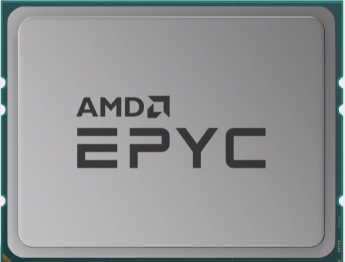
\includegraphics[scale=0.45]{Images/Hardware/amd-epyc.png}
	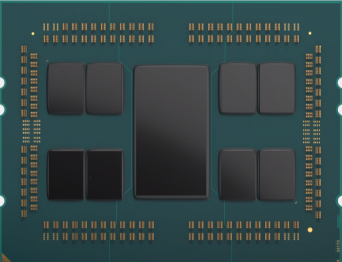
\includegraphics[scale=0.45]{Images/Hardware/amd-epyc-dies.png}
	\decoRule
	\caption[AMD Epyc 7002 series chip]{AMD Epyc 7002 series chip: \href{https://www.amd.com/en/processors/epyc-7002-series}{URL}}
	\label{fig:amd-epyc-7002-chip}
\end{figure}

Graphics Processing Units (GPUs), on the other hand, provide much higher parallelism, while still being relatively easy for their software to be written. However, they can be costly to scale up, and their power consumption can be really high. For reference, at the time of writing, a top-grade GPU for ML, NVIDIA Titan RTX (Figure \ref{fig:nvidia-titan-rtx-explosion-view}), provides up to 72 Streaming Multiprocessors, up to 4,608 CUDA Cores and up to 576 Tensor cores, with a rated base clock of 1,350 MHz and boost clock of 1,770 MHz, 24 GB of Graphics Double Data Rate (GDDR6) Memory and a power consumption of 280 Watts for 2,500 USD \cite{NVIDIA-Titan-RTX-GPU}.

\begin{figure} [H]
	\centering
	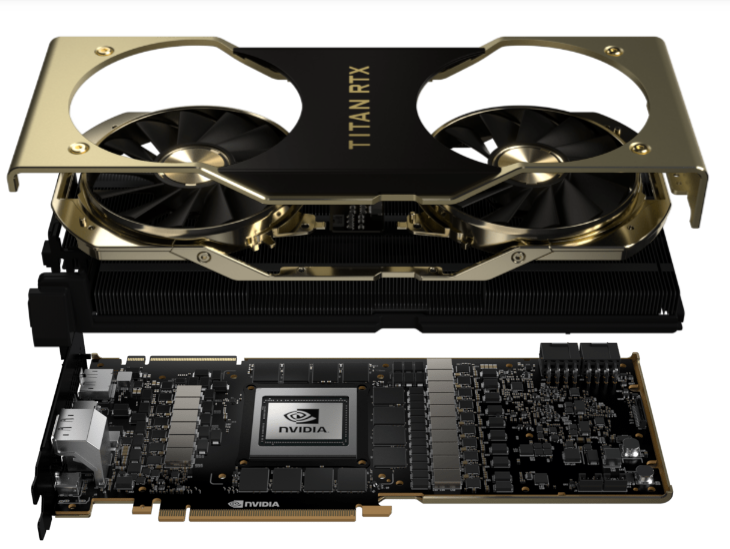
\includegraphics[scale=0.5]{Images/Hardware/NVIDIA-Titan-RTX.png}
	% 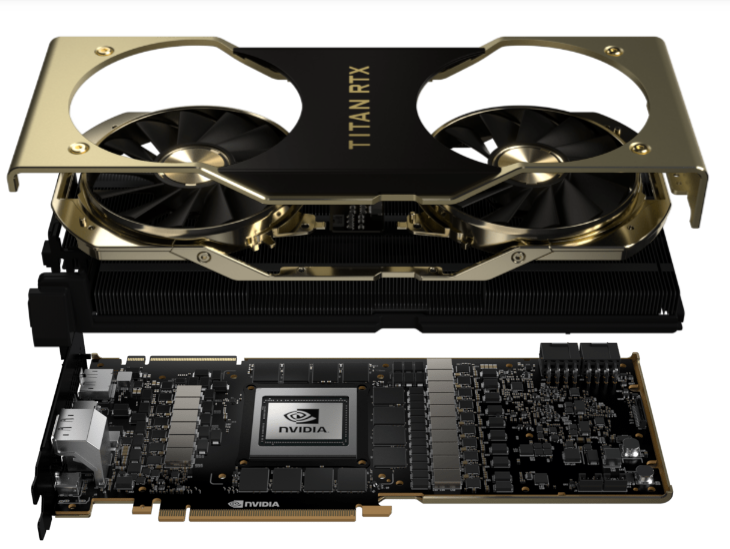
\includegraphics[width=\textwidth]{Images/Hardware/NVIDIA-Titan-RTX.png}
	\decoRule
	\caption[NVIDIA Titan RTX card]{NVIDIA Titan RTX card: \href{https://www.nvidia.com/en-us/deep-learning-ai/products/titan-rtx/}{URL}}
	\label{fig:nvidia-titan-rtx-explosion-view}
\end{figure}

Moreover, there are Application Specific Integrated Circuits (ASICs), which can provide the best parallelism capabilities and the lowest power consumption for a particular application. Unfortunately, they are very expensive to develop and produce, and they can only serve a single purpose, a single application. An example of such an ASIC is the Google Cloud Tensor Processing Unit (TPU) (Figure \ref{fig:google-tpu-motherboard}), which, for the third version (v3), in a single chip there are two TPU cores, each of which contains two scalar, vector, and matrix units (MXUs), and 16 GB of High Bandwidth Memory (HBM) \cite{Google-Cloud-TPU}.

\begin{figure} [H]
	\centering
	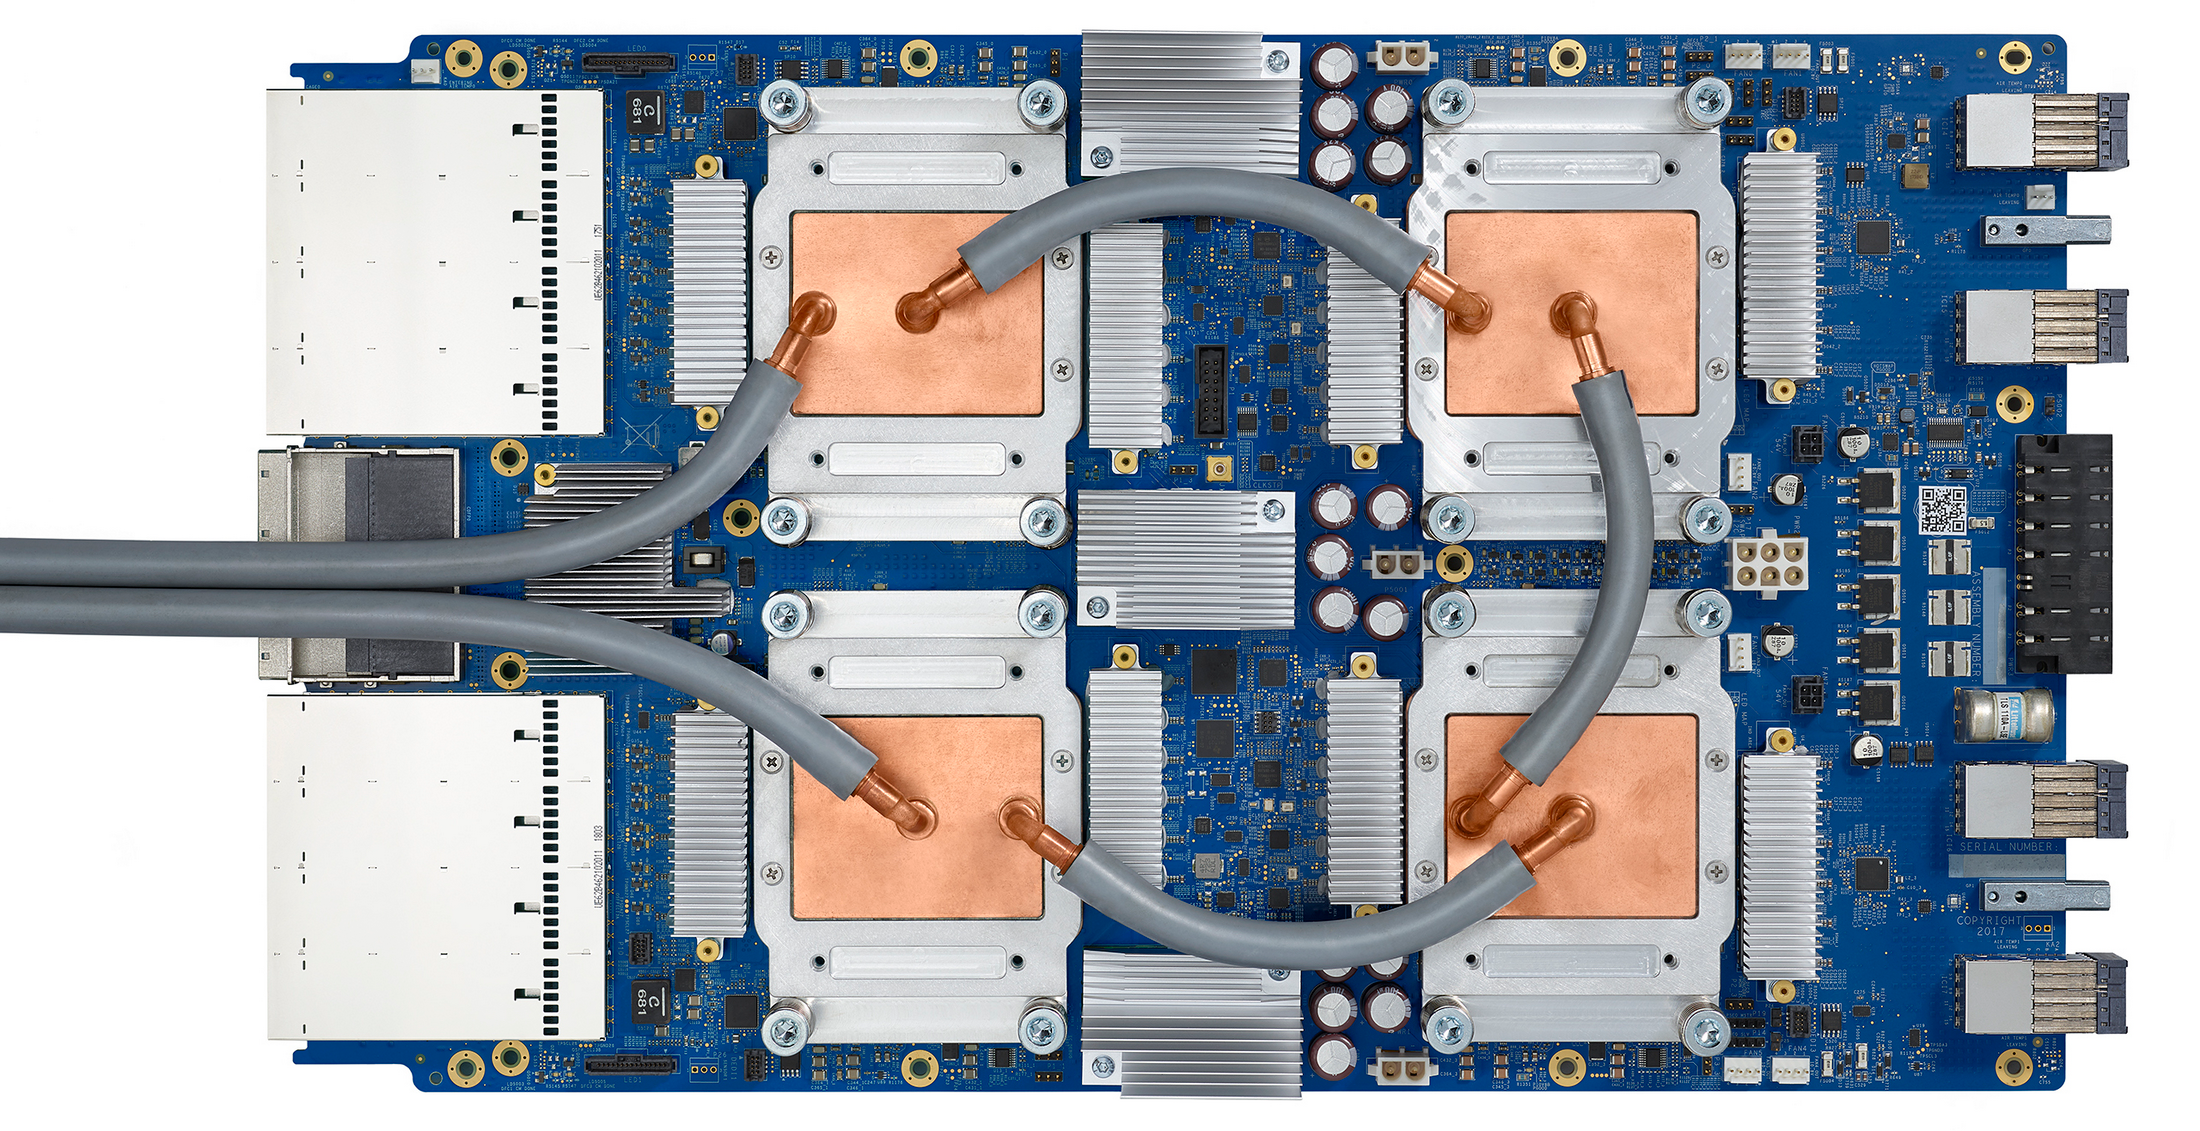
\includegraphics[width=\textwidth]{Images/Hardware/tpu-v3.png}
	\decoRule
	\caption[Google's TPU v3]{Google's TPU v3 - 4 chips, 2 cores per chip: \href{https://cloud.google.com/tpu/docs/system-architecture}{URL}}
	\label{fig:google-tpu-motherboard}
\end{figure}

On the contrary, Field Programmable Gate Arrays (FPGAs) are bridging the gap between the GPUs' flexibility and the ASICs' performance and power consumption. An example FPGA Hardware targeted for High-Performance Computing (HPC) is the Quad-FPGA Daughter Board (QFDB) (Figure \ref{fig:forth-qfdb-daughterboard}) \cite{Implementation-and-Impact-of-an-Ultra-Compact-Multi-FPGA-Board-for-Large-System-Prototyping}, developed by the Foundation of Research and Technology Hellas (FORTH) \cite{FORTH}, combines four interconnected Xilinx Zynq Ultrascale+ Multi-Processor Systems on Chip (MPSoCs), with 16GB of DDR4 memory and an M.2 Solid State Drive (SSD).

\begin{figure} [H]
	\centering
	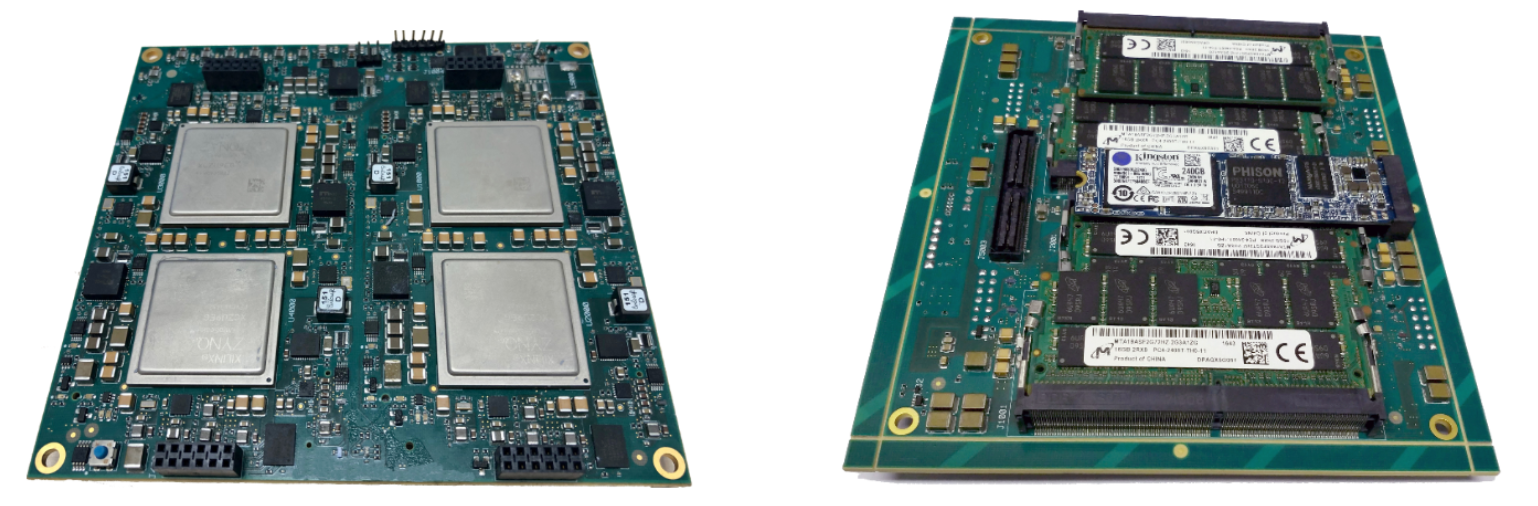
\includegraphics[scale=0.22]{Images/Hardware/QFDB.png}
	% 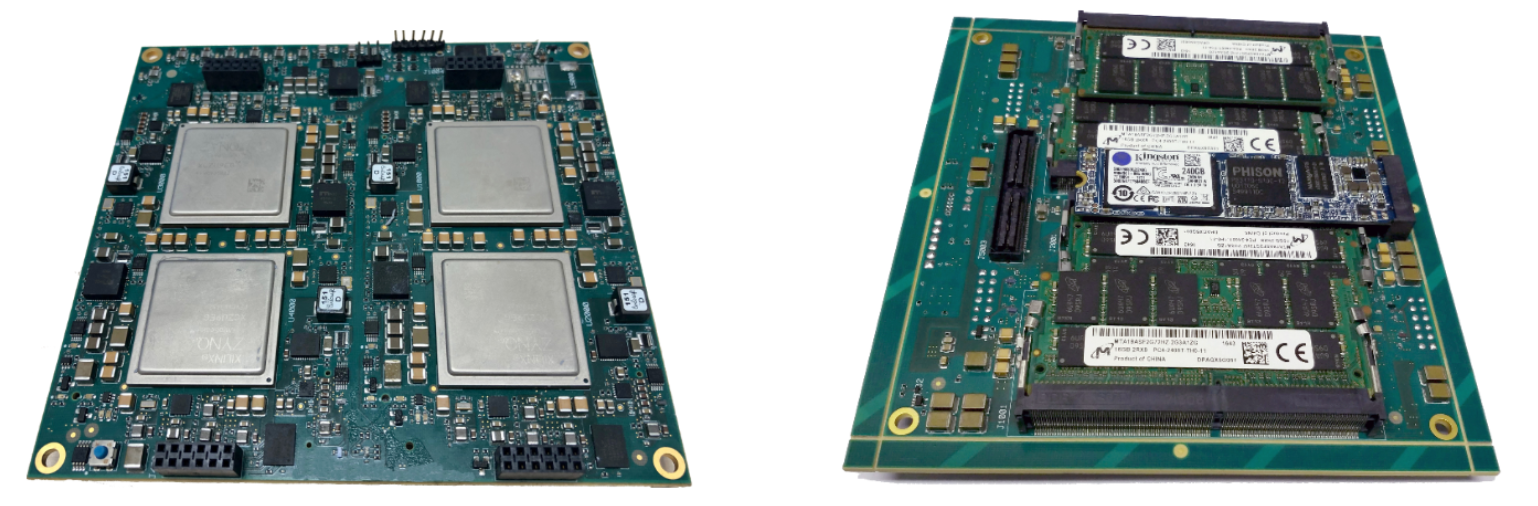
\includegraphics[width=\textwidth]{Images/Hardware/QFDB.png}\\[0.5cm]
	\decoRule
	\caption[FORTH QFDB]{FORTH QFDB, top-view (left) and bottom-view (right): \href{https://ieeexplore.ieee.org/stamp/stamp.jsp?arnumber=8945720}{URL}}
	\label{fig:forth-qfdb-daughterboard}
\end{figure}

In this work, the FPGAs' benefits are being utilized to create a hardware accelerator that can speed up the inference of Convolutional Neural Networks (CNNs), a branch of Deep Neural Networks (DNNs), which is a subfield of Machine Learning.

\section{Scientific Contributions}

\section{Thesis Outline}
% Todo: fill chapter descriptions
\begin{itemize}
	\item \textbf{Chapter 2 - Theoretical Background:} The theoretical background of Machine Learning, with emphasis on Convolutional Neural Networks, is described.
	\item \textbf{Chapter 3 - Related Work:} The related work on the field of Convolutional Neural Networks and their hardware implementations is described.
	\item \textbf{Chapter 4:} Chapter 4 description
	\item \textbf{Chapter 5:} Chapter 5 description
	\item \textbf{Chapter 6:} Chapter 6 description
	\item \textbf{Chapter 7:} Chapter 7 description
\end{itemize}

\chapter{Theoretical Background}

\label{Chapter-Theoretical-Background}

The theoretical background of Machine Learning and Convolutional Neural Networks is being described below.

\section{Machine Learning}
Machine Learning, the name of which was first proposed in 1959 by Arthur Samuel \cite{Some-Studies-in-Machine-Learning-Using-the-Game-of-Checkers}, is a subset of Artificial Intelligence, a Computer Science (CS) field that studies algorithms and statistical models capable of performing specific tasks, such as prediction or decision making, without being explicitly programmed. Instead, sample data are used, also known as "training data", for the machine to "learn" to distinguish useful patterns on the input data capable of creating the needed output, e.g., decision or prediction. There are numerous approaches \cite{Machine-learning-Wikipedia} on the learning algorithms types, as well as on the model types used to get trained.

Such algorithm types, at the time of writing, include, but are not limited to:
\begin{itemize}
	\item \textbf{Supervised Learning:} Algorithms that learn by using "labeled" sample data, data that contain both the inputs and their desired outputs to be used for classification and regression.
	\item \textbf{Unsupervised Learning:} In contrast with the Supervised Learning, unlabeled sample data are used to discover structures that could group or cluster them.
	\item \textbf{Reinforcement Learning:} Algorithms responsible for taking actions in an environment, often also described as software agents, to maximize a specific metric, many of which use dynamic programming techniques.
	\item \textbf{Feature Learning:} Algorithms that by combining or even discarding features from the input samples, try to create a new, more useful set of features. One of the most popular algorithms of this category is Principal Components Analysis (PCA).
	\item \textbf{Anomaly Detection:} Algorithms that try to identify outlier samples, which are characterized by their significant difference compared to the majority of the data used. Such algorithms are often used in noise reduction, data mining, and even security and defense systems.
	\item \textbf{Association Rule Learning:} Algorithms that aim to discover strong relationships between features.
\end{itemize}

Such model types, at the time of writing, include, but are not limited to:
\begin{itemize}
	\item \textbf{Artificial Neural Networks (ANN):} Also known as Connectionist Systems, imitate the biological brain's neural networks.
	\item \textbf{Decision Trees:} Used to make assumptions about the input items' target value (the decision tree's leaves) via its observations (the decision tree's branches). When the target takes continuous values, the Decision Tree is called a Regression Tree.
	\item \textbf{Support Vector Machines (SVM):} Used for classification and regression, most\-ly famous as non-probabilistic, binary, linear classifiers. They can also be used for non-linear classification using the kernel trick.
	\item \textbf{Bayesian Networks:} Represented as directed acyclic graphs, they can include probabilistic relationships.
\end{itemize}

Nowadays, most industries have already used Machine Learning in some sort, indicating the significance and variety of its capabilities. It is estimated \cite{Machine-Learning-Applications} that by the year 2021, AI and ML spending will reach 57.6 Billion USD. Its applications include but are not limited to \cite{Top-Machine-Learning-Applications-in-2019} \cite{Roundup-Of-Machine-Learning-Forecasts-And-Market-Estimates}, web page ranking, image recognition, email filtering, and spam detection, database mining, handwriting recognition, speech recognition, natural language processing, computer vision, image/video/text/speech generation, personalized marketing, traveling, dynamic pricing, healthcare, facial and fingerprint recognition and intrusion detection.

\section{Artificial Neural Network}
It is widely accepted that the brain's most exceptional ability is pattern recognition, which is used to combine "data" from the organism's senses in a way to better understand its environment. Artificial Neural Networks (ANN), a highly popular sub-field of Machine Learning, try to imitate the brain's structure to solve such problems, a structure that has been developing and proving its capabilities for thousands of years.

While ANNs are inspired by biological neural networks, they are not identical. A neural network is a collection of connected neurons, through which electrical signals from sensor organs or other neurons are passed and processed. A biological neuron is comprised of four main parts; Dendrites, Cell body, Axon, and Synaptic terminals (Figure \ref{fig:Standard-structure-of-a-biological-neuron}). A Dendrite and its Dendritic branches are used as the neuron's input, where sensors or other neurons get connected. A neuron can have multiple Dendrites. The neuron's cell body collects all the input signals and applies an "activation" function to create the output signal. Afterward, the output signal is transported through the Axon and then distributed to the next neurons through the Synaptic terminals. The Synaptic terminals to Dendrites connections are called Synapses.

\begin{figure} [H]
	\centering
	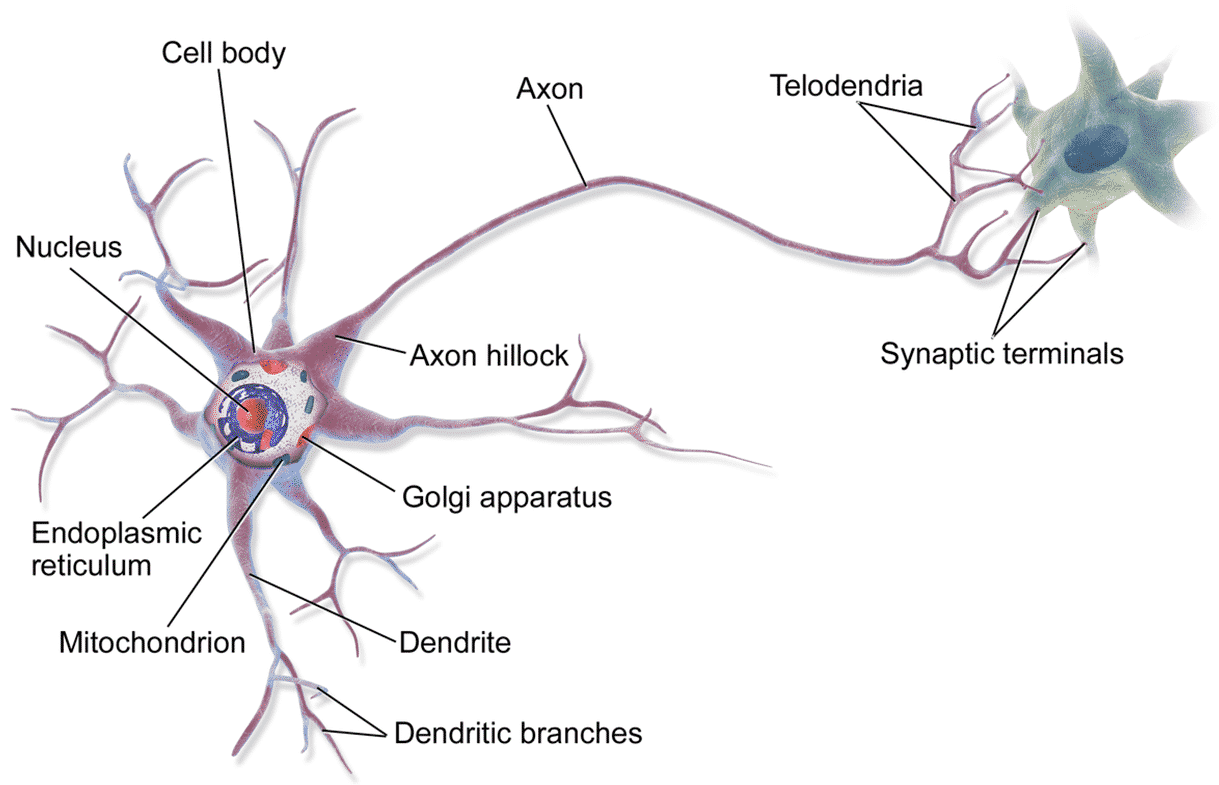
\includegraphics[scale=0.25]{Images/Biological-Neuron.png}
	\decoRule
	\caption[Standard structure of a biological neuron]{Standard structure of a biological neuron: \href{https://nurseslabs.com/nervous-system/}{URL}}
	\label{fig:Standard-structure-of-a-biological-neuron}
\end{figure}

\subsection{ANNs Basic components} \label{subsection:ANNs-Basic-components}
Similarly to the biological neural networks, an ANN can be represented as a directed, weighted graph (Figure \ref{fig:simplified-neural-network-graph}), whose vertices represent the biological neurons' cell bodies and its edges the biological synapses. The electrical signal used in biological neurons can be represented as a real number, and their outputs can be calculated by some non-linear function of the inputs' weighted sum. Each edge typically can have a weight, set during the training process, which amplifies or weakens the vertex's signal.

\begin{figure} [H]
	\centering
	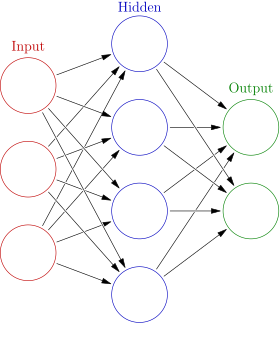
\includegraphics[scale=0.5]{Images/simplified-neural-network-graph.png}
	\decoRule
	\caption[Activation Function Graphs]{Simplified Neural Network Graph: \href{https://en.wikipedia.org/wiki/Artificial_neural_network}{URL}}
	\label{fig:simplified-neural-network-graph}
\end{figure}

\subsubsection{Neuron}
A neuron receives real numbers as inputs, which then using an activation function, are combined with their internal state, also known as activation, and an optional threshold in order to produce the neuron's output.

\subsubsection{Connections and Weights}
Each neuron can be connected with multiple other neurons to be used as inputs and to feed them with its output. Each connection is characterized by its weight, which represents its relative importance.

\subsubsection{Propagation Function}
The propagation function calculates the weighted sum of each neuron's inputs and adds a bias term.

\subsubsection{Activation Function}
The activation function receives the propagation function's result and applies a transformation, which creates the neuron's final output. There are a lot of different activation functions, with specific characteristics for the training and inference process. However, they all provide a smooth and differentiable transition as the input values change. The most commonly used ones are shown below \cite{Activation-Function-Wikipedia}.
\begin{itemize}
	\item \textbf{Identity:} $f(x) = x$\\
	No transformation is applied.

	\item \textbf{Binary Step:} $
		      f(x) =
		      \begin{cases}
			      0 & x \leq 0 \\
			      1 & x > 0
		      \end{cases}
		  $\\
		  While being the original activation function developed when neural networks were invented, it is no longer used as it is incompatible with backpropagation. Backpropagation is the process of updating the weights during the training phase using the gradient descent algorithm. The binary step function is not convex; hence, gradient descent is unable to find a local minimum.

	\item \textbf{Logistic (Sigmoid or Soft step):} $
		      f(x) = \sigma(x) = \frac{1}{1 + e^{-x}}
		  $\\
		  Often used, however, in real-world neural networks, it is avoided due to the vanishing gradient problem \cite{The-Vanishing-Gradient-Problem-During-Learning-Recurrent-Neural-Nets-and-Problem-Solutions}.

	\item \textbf{TanH:} $
		      f(x) = tanh(x) = \frac{e^{x} - e^{-x}}{e^{x} - e^{-x}}
		  $\\
		  Same as Logistic.

	\item \textbf{Rectified Linear Unit (ReLU):} $
		      f(x) =
		      \begin{cases}
			      0 & x < 0 \\
			      x & x > 0
		      \end{cases}
		  $\\
		  The most popular activation function, due to its fast backpropagation speeds, its low penalty on generalization accuracy, and its resistance to saturation conditions \cite{ImageNet-Classification-Using-Binary-Convolutional-Neural-Networks}.

	\item \textbf{Softmax:} $
		      f_i(\textbf{x}) = \frac{
		      e^{x_i}
		      }{
		      \sum_{j=1}^{J}e^{x_j}
		      }
		  $, for i = 1, ..., J\\
		  Commonly used as a final output activation function for multiclass classification. It normalizes the output to [0, 1], and makes the outputs' sum equal to 1. After this transformation, the i-th output's value designates the probability of the input to be the class i.
\end{itemize}

\begin{figure} [H]
	\centering
	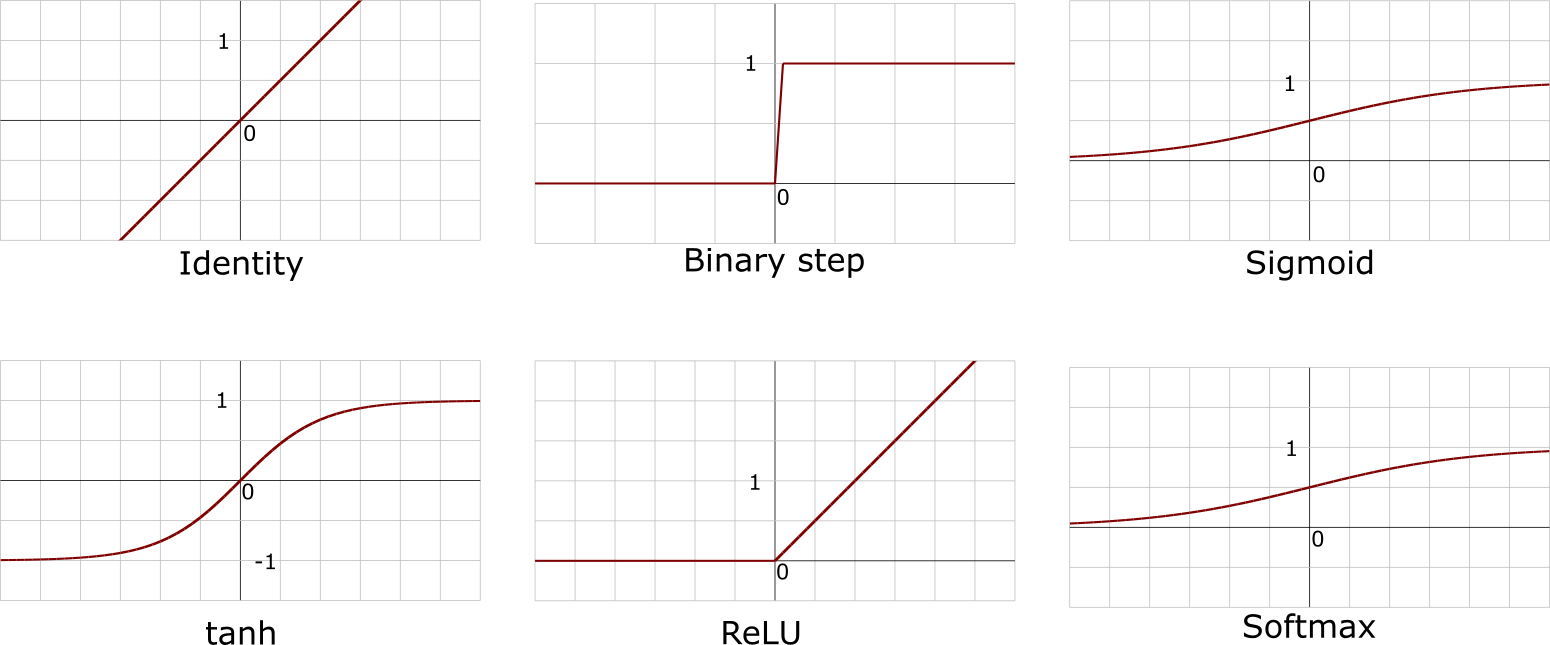
\includegraphics[width=\textwidth]{Images/Activation_functions.png}
	\decoRule
	\caption[Activation Function Graphs]{Activation Function Graphs}
	\label{fig:activation-functions}
\end{figure}

\subsection{Organization}
An ANN's neurons are typically organized into groups, called layers, in which each neuron has the same distance from the inputs as all the other neurons of its group. The input layer is the layer that gets as inputs the external data, and the output layer, the last layer in the graph, is the one that produces the final output results. Any in-between layer is called a hidden layer. An ANN is called a Deep Neural Network (DNN), when, by convention, it has three or more hidden layers.

\subsection{ANN Architectures}
There are many ANN architectures, each one serving different use cases. They are separated into two main groups, Feedforward networks and Recurrent networks \cite{Types-of-Artificial-Neural-Networks}.

\subsubsection{Feedforward Networks}
The basic idea with the feedforward networks is that the data flows from the input layer through the hidden layers to the output layer without any cycles, so they can be represented as directed, acyclic graphs. Some architectures of this group are:
\begin{itemize}
	\item Multiclass Perceptron
	\item Group method of data handling
	\item Autoencoder
	\item Probabilistic
	\item Time delay
	\item Convolutional
	\item Deep stacking network
\end{itemize}

\subsubsection{Recurrent Networks}
Recurrent Neural Networks (RNN), similarly to the Feedforward networks, data flows from the input layer through the hidden layers to the output layer. However, they allow for data cycles, in other words, outputs of the $layer_n$ can be fed to the inputs of the $layer_{n-1}$, so they can be represented as directed, cyclic graphs. Some architectures of this group are:
\begin{itemize}
	\item Fully recurrent
	\item Simple recurrent
	\item Reservoir computing
	\item Long short-term memory
	\item Bi-directional
	\item Hierarchical
	\item Stochastic
	\item Genetic Scale
\end{itemize}
For every ANN Architecture, there are specific types of layers that apply different kinds of mathematical operations on their input data. Each layer type has characteristics on the way its mathematical operations are applied to its input. Those characteristics are generally called hyperparameters. For example, in a Fully-Connected layer, a hyperparameter is its number of outputs. Hyperparameters are set by the engineers during the training phase, which are fine-tuned, concerning the application's input data.

This work is focused on the Convolutional Neural Networks (CNN), which are described in detail below.

\section{Convolutional Neural Networks}
Convolutional Neural Networks (CNNs) are deep feedforward neural networks that specialize in processing data with grid-like topologies and are typically used in visual imagery analysis. They are simple neural networks that, for at least one of their layers, use the convolution mathematical operation instead of the general matrix multiplication \cite{Goodfellow-et-al-2016}.

CNNs imitate the brain's visual cortex, which is the area responsible for the visual processes. Cortical neurons cover small areas of the visual field, with partial overlaps resulting in full visual field coverage.

CNNs most significant advantage over other image classification algorithms is their little need for pre-processing, meaning that their filters are learned during the training phase while using traditional algorithms, they have to be hand-engineered.

Some of their applications are image and video recognition, image classification, object detection, recommendation systems, medical image analysis, natural language processing, and financial time series \cite{Convolutional-neural-networks-wikipedia}.

\subsection{Structure}
A typical CNN consists of two parts. The first part includes multiple convolutional and pooling layers, which extract features from the given input. The second part, also known as the classifier, includes multiple fully connected layers, which classify the given input using the features extracted from the first part (Figure \ref{fig:typical-cnn-architecture}).

\begin{figure} [H]
	\centering
	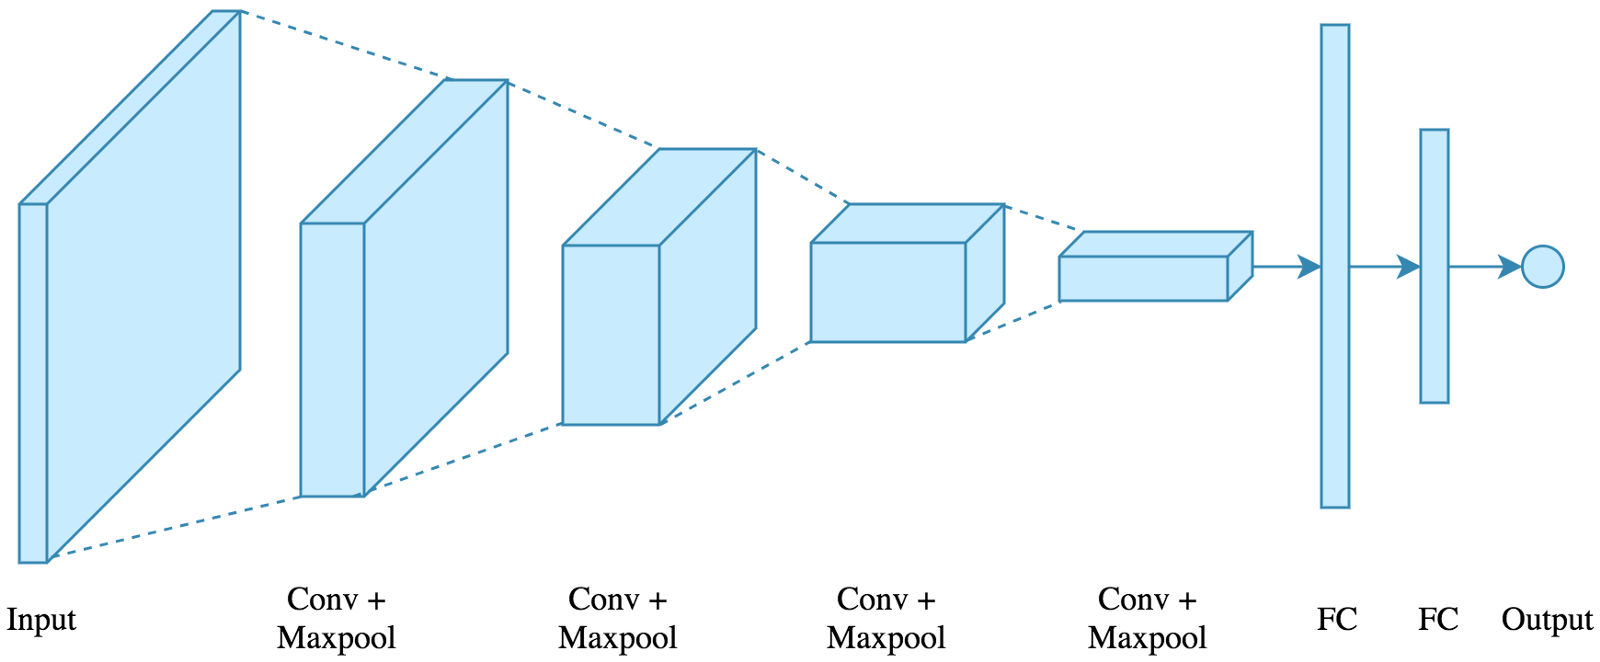
\includegraphics[width=\textwidth]{Images/typical-cnn-architecture.png}
	\decoRule
	\caption[Typical CNN Architecture]{Typical CNN Architecture - First five layers (Convolution + Max Pooling layers) used for feature extraction, last three layers (Fully-Connected) used for classification, also called the classifier: \href{https://www.kaggle.com/mauddib/digit-recogniser-tutorial-using-a-cnn-tensorflow}{URL}}
	\label{fig:typical-cnn-architecture}
\end{figure}

The input data is typically structured as multidimensional arrays, also known as tensors. For example, if the input data are RGB images, then the input tensor's shape is (number of images) x (image width) x (image height) x (image depth), where image depth is called the image's color channels, in this example 3 channels. Moreover, the input data can also be grayscale images or even hyperspectral images. Hyperspectral images have multiple color channels, even in the non-visible for the human eye spectrum, with applications including the medical and space fields. There are also implementations such as 1D and 3D CNNs, but this work examines 2D CNNs only.

The trainable parameters (weights and biases) needed for the computation are initially assigned random values \cite{Practical-recommendations-for-gradient-based-training-of-deep-architectures}, rendering the network useless. However, during the training phase, using the backpropagation process \cite{Learning-internal-representations-by-error-propagation}, those weights are being optimized to form features from the training set. The trainable parameters are also considered to be shared \cite{Generalization-and-network-design-strategies}, meaning that the same parameters are to be used in the entirety of the input data, dramatically decreasing their number and consequently their memory footprint and also increasing the network robustness against overfitting.

As stated above, there are three types of layers used in 2D CNNs; Convolutional, Pooling, and Fully-Connected layers. Each layer is being described below.

\subsubsection{Convolutional Layer}
A convolutional layer creates and outputs a similarity map between the input data and the convolution's filters, also known as kernels. More specifically, every filter is convolved across the input's width and height, producing the dot product of them. The result is multiple two-dimensional arrays, whose each cell holds the similarity of each filter to some spatial position in the input.

Each filter is a specific type of feature, depending on the training set. For example, in image classification, a filter can be a rough shape of cats' mustaches, so that after the convolution, it can be indicated if they are contained somewhere in the input image. If they are, then, to some probability defined during the training phase, there might be a cat in the input image.

Each convolutional layer is defined by its hyperparameters. Those are:
\begin{itemize}
	\item \textbf{Kernel size:} The width and height of the kernels' (filters') size, typically, small\-er than the given input.
	\item \textbf{Output channels:} The number of feature maps to be created as outputs. Consequently, the number of kernels to be used in this operation also equals to the output channels number.
	\item \textbf{Stride:} The number of pixels to be skipped horizontally and vertically in each partial convolution. Typically, this number does not differ between the two dimensions.
	\item \textbf{Zero padding:} There might be a need for zero-padding the input to include as much data as possible in the final computation. There are three different ways of padding:
	      \begin{itemize}
		      \item \textbf{Valid:} No padding is applied; some data may not be included in the computation.
		      \item \textbf{Same:} Applies the amount of padding needed to result in the same width and height as the input.
		      \item \textbf{Full:} Applies padding on the input's edges with a specified number of pixels per dimension.
	      \end{itemize}
\end{itemize}

The mathematical expression of the convolution operation is defined bellow (Equation \ref{eqn:convolution}) and visualized on Figure \ref{fig:convolution-operation}.

Let \emph{I} be the input with \emph{C} channels, \emph{H} height and \emph{W} width, and let \emph{K} be the kernels with \emph{N} number of kernels, \emph{C} channels, \emph{KH} height and \emph{KW} width. Also, let \emph{B} be the bias with K values, and let \emph{S} be the stride size and \emph{P} be the padding size. So the convolution operation's output, \emph{Out}, is defined as:
\begin{equation}
	% Todo: fix overfull hbox
	I_{padded}(c, i, j) = \begin{cases}
		0,                  & i \in [1, P], j \in [1, P]                         \\
		I(c, i - P, j - P), & i \in [P + 1, P + 1 + H], j \in [P + 1, P + 1 + W] \\
		0,                  & i \in [H + 1, H + 1 + P], j \in [W + 1, W + 1 + P] \\
	\end{cases}
\end{equation}

\begin{equation}
	OH = \frac{H + 2P - KH}{S} + 1
\end{equation}

\begin{equation}
	OW = \frac{W + 2P - KW}{S} + 1
\end{equation}

\begin{equation}
	\label{eqn:convolution}
	% Todo: fix overfull hbox
	\begin{split}
		Out(k, i, j) = B(k) +
		\sum_{c = 1}^{C} \sum_{kh = 1}^{KH} \sum_{kw = 1}^{KW}
		I_{padded}(c, kh + i * KH, kw + j * KW) K(k, c, kh, kw),\\
		\mbox{for k = 1, 2, ..., C},\\
		\mbox{for i = 1, 2, ..., OH},\\
		\mbox{for j = 1, 2, ..., OW}\\
	\end{split}
\end{equation}

\begin{figure} [H]
	\centering
	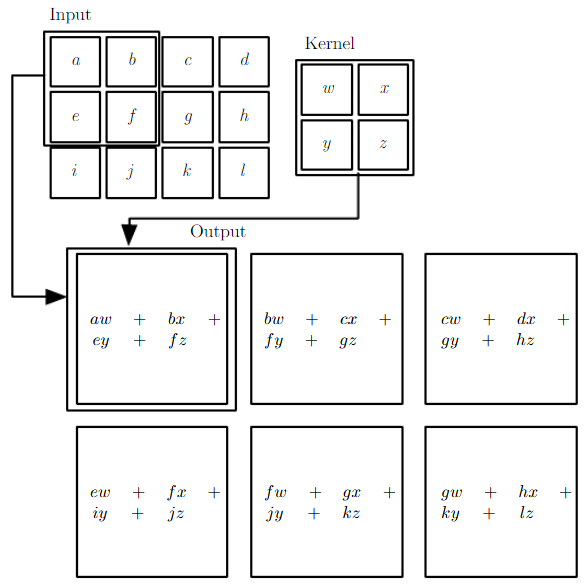
\includegraphics[scale=0.6]{Images/CNNArchitectures/convolution-operation.png}
	% 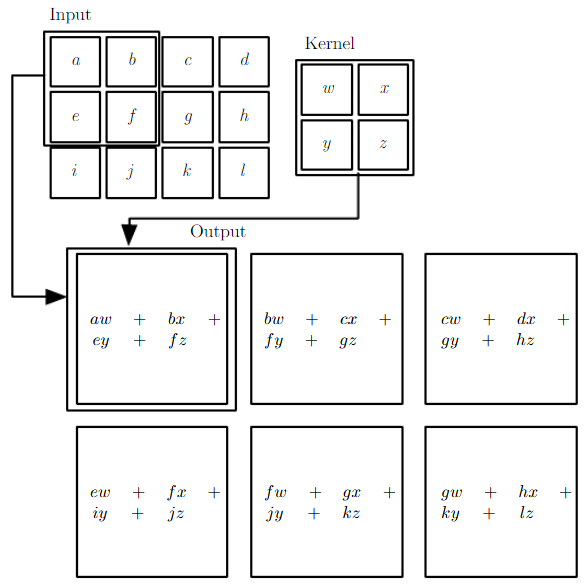
\includegraphics[width=\textwidth]{Images/CNNArchitectures/convolution-operation.png}
	\decoRule
	\caption[Convolution Operation]{Convolution Operation - A 2x2 Kernel filter is applied on the 4x3 example input matrix with stride 1 and valid padding. Figure from \cite{Goodfellow-et-al-2016}.}
	\label{fig:convolution-operation}
\end{figure}

Nowadays, most applications might require multiple Convolutional layers to extract useful features from their complex inputs. Deeper architectures, in general, create more detailed characteristics. Furthermore, activation functions can be interjected between adjacent Convolutional layers to enhance the network's nonlinearity. Activation functions can make the network function as a universal function approximator \cite{Approximation-capabilities-of-multilayer-feedforward-networks}.

\subsubsection{Pooling Layer}
A pooling layer sub-samples its input not only to decrease the computation footprint needed for the next layer, but also to make the network more prone to over-fitting. It reduces the input dimensions by combining multiple neurons into a single neuron. Max-Pooling layers combine groups of neurons by outputting their maximum value. Average-Pooling layers combine groups of neurons by outputting their average value.

Similarly to the convolutional layer, a pooling layer slides a window of some size, called kernel size, across the input data. The data to be combined are those that the sliding window has selected. In 2D CNNs, the pooling layers have 2D windows; the channels are not combined.

A pooling layer can be local, combining small groups of neurons, which also means that the layer's kernel size is small compared to the input size. It can also be global, combining the whole input to a single neuron.

Each pooling layer is defined by its hyperparameters. Those are:
\begin{itemize}
	\item \textbf{Kernel size:} The kernel's (sliding window's) width and height.
	\item \textbf{Stride:} The number of pixels to be skipped horizontally and vertically in each slide. Typically, this number does not differ between the two dimensions.
\end{itemize}

The mathematical expression of the average-pooling operation (Equation \ref{eqn:avg-pooling}) and max-pooling operation (Equation \ref{eqn:max-pooling}) is defined and visualized (Figure \ref{fig:max-pooling-operation}) bellow.

Let \emph{I} be the input with \emph{C} channels, \emph{H} height and \emph{W} width, let \emph{KH} be the kernel's height, let \emph{KW} be the kernel's width, and let \emph{S} be the stride size. So the pooling operations are defined as:
\begin{equation}
	OH = \frac{H - KH}{S} + 1
\end{equation}

\begin{equation}
	OW = \frac{W - KW}{S} + 1
\end{equation}

\begin{equation}
	\label{eqn:avg-pooling}
	\begin{split}
		AvgPool(c, i, j) =
		\frac{
			\sum_{kh = 1}^{KH} \sum_{kw = 1}^{KW}
			I(c, kh + i * KH, kw + j * KW)
		}{
			KH * KW
		},\\
		\mbox{for c = 1, 2, ..., C},\\
		\mbox{for i = 1, 2, ..., OH},\\
		\mbox{for j = 1, 2, ..., OW}\\
	\end{split}
\end{equation}

\begin{equation}
	\label{eqn:max-pooling}
	\begin{split}
		MaxPool(c, i, j) = \max_{1 \leq kh \leq KH, 1 \leq kw \leq KW}
		I(c, kh + i * KH, kw + j * KW),\\
		\mbox{for c = 1, 2, ..., C},\\
		\mbox{for i = 1, 2, ..., OH},\\
		\mbox{for j = 1, 2, ..., OW}\\
	\end{split}
\end{equation}

\begin{figure} [H]
	\centering
	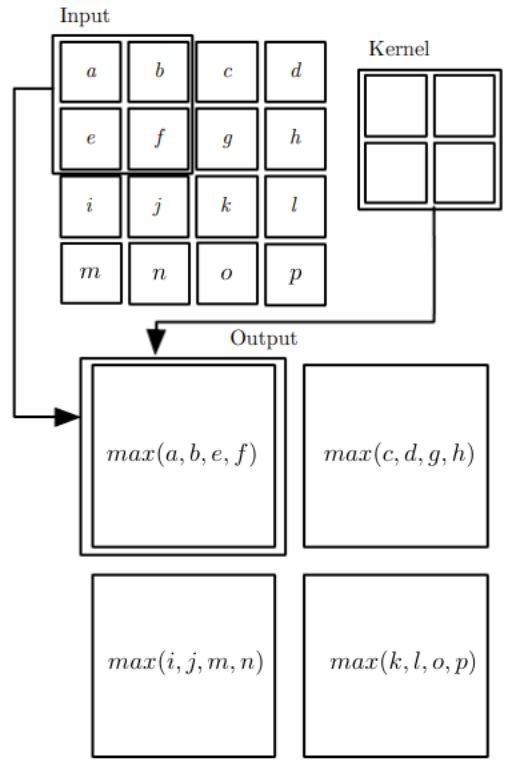
\includegraphics[scale=0.6]{Images/CNNArchitectures/maxpooling-operation.png}
	% 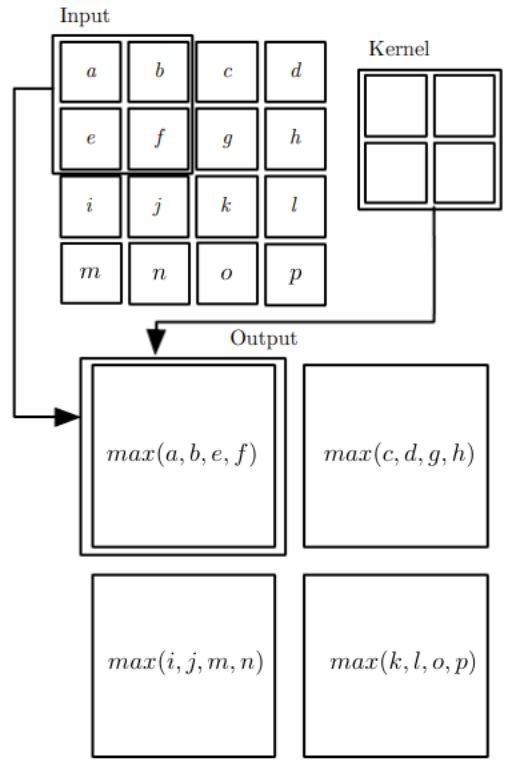
\includegraphics[width=\textwidth]{Images/CNNArchitectures/maxpooling-operation.png}
	\decoRule
	\caption[Max-Pooling Operation]{Max-Pooling Operation - A max operation is applied with a 2x2 Kernel on the 4x4 example input matrix with stride 2. Figure from \cite{Goodfellow-et-al-2016}.}
	\label{fig:max-pooling-operation}
\end{figure}

\subsubsection{Fully-Connected Layer}
The CNNs classifier part is comprised of several Fully-Connected layers, which serve as the high-level reasoning. It is the part that finally classifies the given input.

A Fully-Connected layer is the simplest type of layer, as it is the one used in Multi-Layer Perceptron (MLP) neural networks. More specifically, it receives input, with which it computes a weighted sum for each of its output values. This input is derived from the flattened output of several convolutional and pooling layers.

Each Fully-Connected layer is defined by its hyperparameters. Those are:
\begin{itemize}
	\item \textbf{Output Features:} The number of features to output. Consequently, this also configures the number of weights needed for the computation, hence, its memory and computation footprint.
\end{itemize}

The mathematical expression of the Fully-Connected layer's operation (Equation \ref{eqn:fully-connected}) is defined bellow.

Let \emph{I} be the input with \emph{N} input features, let \emph{W} be the layers weights, let \emph{B} be the layer's bias, and let \emph{M} be the layer's output features. So the Fully-Connected layer's output, \emph{Out}, is defined as:
\begin{equation}
	\label{eqn:fully-connected}
	Out(i) = B(i) + \sum_{j = 1}^{N} I(j)W(i, j), \mbox{for i = 1, 2, ..., M}
\end{equation}

The parameters' reuse of Fully-Connected layers from a specific application to another cannot be done since they are strictly bonded to the classes and high-level features of the particular Convolutional neural network.

The final Fully-Connected layers is typically followed by a Softmax activation layer, which, as stated on section \ref{subsection:ANNs-Basic-components}, it calculates the probability of the input being a certain class. The use of Softmax enables the confidence quantification for every estimation, and easy troubleshooting when the input it misclassified.

\subsubsection{Activation Layer}
After each Convolutional and Fully-Connected layer, there can be an Activation layer, which applies an activation function on the output of its previous layer. An activation layer increases the network's nonlinearity without affecting the convolutional layers' receptive fields. The activation function can be one of those presented in section \ref{subsection:ANNs-Basic-components}, but ReLU and its variants are generally preferred, due to its fast training characteristics and its low penalty on generalization accuracy.

\section{Theoretical knowledge sources}
The aforementioned theoretical background was mostly obtained from the Statistical Modeling and Pattern Recognition course of Electrical and Computer Engineering school at the Technical University of Crete. In addition, the book Deep Learning \cite{Goodfellow-et-al-2016} was used when finer details were needed. Moreover, the Udacity course Intro to Deep Learning with PyTorch by Facebook AI \cite{Udacity-Intro-to-Deep-Learning-with-PyTorch-by-Facebook-AI} was used for a more hands-on approach, focusing on PyTorch and Python in general. Last but not least, a great resource has been all the papers mentioned above.

\chapter{Related Work}

\label{Chapter-Related-Work}

\section{ImageNet}


\section{GPU Approach}

\section{Google Brain Project}
\subsection{DistBelief}
\subsection{TensorFlow}
\subsection{Tensor Processing Unit (TPU)}

\section{The FPGA Perspective}
\subsection{Xilinx CHaiDNN}
\subsection{Xilinx Deep Learning Processor Unit (DPU)}

\section{Thesis Approach}

\chapter{Robustness Analysis}

\label{Chapter-Robustness-Analysis}

In this chapter, AlexNet's \cite{ImageNet-classification-with-deep-convolutional-neural-networks} structure is analyzed and modeled using MATLAB \cite{MATLAB-Official-site} and C/C++, evaluating the results using PyTorch \cite{PyTorch-Official-site}. As a starting point, the prebuilt and pre-trained AlexNet model provided by PyTorch was used. For a better understanding of the underlining algorithms, a C/C++ library was created to replicate PyTorch's functionality, from image and parameter importing and formatting, to every CNN layer type needed for the network's inference.

Moreover, a Sensitivity Analysis was performed to explore hardware implementation opportunities. Furthermore, various quantization techniques and algorithmic optimizations have been studied and tested to reduce memory footprint and better utilize hardware resources. Lastly, several implementation techniques and tools on the same functionality have been studied to minimize hardware resources and latency.

\section{PyTorch and C/C++ implementations}
Since PyTorch is a high abstraction framework, the recreation of its functionality to a lower abstraction level language, like C/C++, is a necessity for a complete understanding of the neural network's operation mechanism. Hence, after creating a C/C++ library capable of implementing most CNNs, it was evaluated for its correctness using PyTorch as a baseline. Its evaluation was conducted by implementing AlexNet as an example network, using both PyTorch and the C/C++ library, and then running the network's inference on both implementations. A subset of the ImageNet's database was used as input images, provided by Kaggle \cite{Kaggle}, which included 1250 images of cats and another 1250 images of dogs.

Afterward, the results, taken from the last FC layer of both implementations, were compared to create an error rate for each input. The library is designed in a way that it can use any data type for weights and activations to enable further experimentations. This evaluation experiment was conducted two times, one for using double-precision and another for using single-precision floating-point data type (IEEE standard). The error rate of both experiments was almost zero, with some minor inconsistencies between the floating-point representations of C/C++ and Python. Thus, both implementations' classifications were fully matched, and the library can be characterized as correct.

\subsection{Algorithms}
The main building blocks of a typical 2-D CNN is presented below.

\subsubsection{Convolution}
Algorithm \ref{alg:Convolution-Layer} performs a 2-D Convolution on 3-D array inputs, like images. The \textit{input} is characterized by its height, its width, and its number of channels. In other words, the number of its parallel matrices; for an RGB image, there are three channels, one for every color. The \textit{kernelSize}, \textit{stride} and \textit{padding} are the hyper-parameters of convolution layers, and because they differ for every layer and network, they have to be included in the procedure's parameters. Last but not least, \textit{weights} and \textit{bias} are the networks parameters. This algorithm outputs a 3-D array with the convolution's results.

\begin{algorithm}[H]
	\caption{Convolution Layer}\label{alg:Convolution-Layer}
	\begin{algorithmic}[1]
		\Procedure{Convolution Layer}{input, kernelSize, stride, padding, weights, bias}
			\State $hOut \gets (input.height +2 * padding - kernelSize) / stride + 1$
			\State $wOut \gets (input.width +2 * padding - kernelSize) / stride + 1$

			\For{i:=1 \textbf{to} input.channels}
				\For{j:=1 \textbf{to} input.height + 2 * padding}
					\For{k:=1 \textbf{to} input.width + 2 * padding}
						\If{j < padding || k < padding || j > image.height || k > image.height}
							\State $arr(i, j, k) \gets 0$
						\Else{}
							\State $arr(i, j, k) \gets input(i, j - padding, k - padding)$
						\EndIf
					\EndFor
				\EndFor
			\EndFor

			\For{oc:=1 \textbf{to} size(weights, 1)} \Comment{\#Output channels}
				\For{oh:=1 \textbf{to} hOut}
					\State $imgStartH \gets oh * stride$
					\State $imgEndH \gets imgStartH + kernelSize$

					\For{ow:=1 \textbf{to} wOut}
						\State $imgStartW \gets ow * stride$
						\State $imgEndW \gets imgStartW + kernelSize$

						\State $pixel \gets 0$
						\For{ic:=1 \textbf{to} input.channels}
							\For{i:=1 \textbf{to} kernelSize}
								\For{j:=1 \textbf{to} kernelSize}
									\State $pixel \gets pixel + arr(ic, i + imgStartH, j + imgStartW) * weights(oc, ic, i, j)$
								\EndFor
							\EndFor
						\EndFor

						\State $output(oc, oh, ow) \gets pixel + bias(oc)$
					\EndFor
				\EndFor
			\EndFor
			\State \textbf{return} $output$
		\EndProcedure
	\end{algorithmic}
\end{algorithm}

Algorithm \ref{alg:Convolution-Layer-with-ReLU} is a slightly more optimized version of algorithm \ref{alg:Convolution-Layer}. Since padding creates areas of the input that are zeroed out, convolution on those areas results in zero. Therefore, the for-loops' indices are carefully calculated to avoid iterations on the padded areas. Furthermore, the creation of the "padded" input is also omitted.

Moreover, a small optimization is injecting the ReLU activation function into this algorithm. Provided that ReLU is used almost after every convolution layer, this optimization avoids rereading the whole input from memory to make a simple decision. The procedure's \textit{doRelu} parameter configures if the ReLU activation is used.

\begin{algorithm}[H]
	\caption{Convolution Layer with ReLU}\label{alg:Convolution-Layer-with-ReLU}
	\begin{algorithmic}[1]
		\Procedure{Convolution Layer with ReLU}{input, kernelSize, stride, padding, weights, bias, doRelu}
			\State $hOut \gets (input.height +2 * padding - kernelSize) / stride + 1$
			\State $wOut \gets (input.width +2 * padding - kernelSize) / stride + 1$

			\For{oc:=1 \textbf{to} size(weights, 1)} \Comment{\#Output channels}
				\For{oh:=1 \textbf{to} hOut}

					\State $imgStartH \gets oh * stride - padding$

					\State $iStart \gets imgStartH < 0 ? padding : 0$

					\If{$imgStartH + kernelSize \geq input.height$}
						\State $iEnd \gets kernelSize - (imgStartH + kernelSize - input.height)$
					\Else{}
						\State $iEnd \gets kernelSize$
					\EndIf

					\For{ow:=1 \textbf{to} wOut}
						\State $imgStartW \gets ow * stride - padding$

						\State $jStart \gets imgStartW < 0 ? padding : 0$

						\If{$imgStartW + kernelSize \geq input.height$}
							\State $jEnd \gets kernelSize - (imgStartW + kernelSize - input.height)$
						\Else{}
							\State $jEnd \gets kernelSize$
						\EndIf

						\State $pixel \gets bias(oc)$

						\For{ic:=1 \textbf{to} input.channels}
							\For{i:=iStart \textbf{to} iEnd}
								\For{j:=jStart \textbf{to} jEnd}
									\State $pixel \gets pixel + input(ic, i + imgStartH, j + imgStartW) * weights(oc, ic, i, j)$
								\EndFor
							\EndFor
						\EndFor

						\State $output(oc, oh, ow) \gets doRelu \&\& pixel < 0 ? 0 : pixel$
					\EndFor
				\EndFor
			\EndFor
			\State \textbf{return} $output$
		\EndProcedure
	\end{algorithmic}
\end{algorithm}

\subsubsection{MaxPool}
Algorithm \ref{alg:MaxPool-Layer} performs a 2-D max-pooling operation on 3-D array inputs. Likewise to the convolution algorithm's \textit{input}, it is characterized by its height, width, and channel number. Also the \textit{kernelSize} and \textit{stride} hyper-parameters are present, in contrast to padding, which is not used, so it is omitted. This algorithm outputs a 3-D array with the max-pooling operation's results.

\begin{algorithm}[H]
	\caption{MaxPool Layer}\label{alg:MaxPool-Layer}
	\begin{algorithmic}[1]
		\Procedure{MaxPool Layer}{input, kernelSize, stride}
			\State $hOut \gets (input.height - kernelSize) / stride + 1$
			\State $wOut \gets (input.width - kernelSize) / stride + 1$
			\For{i:=1 \textbf{to} input.channels}
				\For{j:=1 \textbf{to} hOut}
					\For{k:=1 \textbf{to} wOut}
						\State $max \gets -\infinity$
						\For{l:=1 \textbf{to} kernelSize}
							\For{m:=1 \textbf{to} kernelSize}
								\State $curHeight \gets j * stride + l$
								\State $curWidth \gets k * stride + l$
								\State $curPixel \gets input(i, curHeight, curWidth)$
								\If{max < curPixel}
									\State $max \gets curPixel$
								\EndIf
							\EndFor
						\EndFor
						\State $output(i, j, k) \gets max$
					\EndFor
				\EndFor
			\EndFor
			\State \textbf{return} $output$
		\EndProcedure
	\end{algorithmic}
\end{algorithm}

\subsubsection{Fully-Connected}
Algorithm \ref{alg:Fully-Connected-Layer} performs a matrix multiplication on the \textit{input} and \textit{weights}. The \textit{input} is a vector, either coming from the previous FC layer's output or the flattening of the previous convolution or max-pooling layer's results. After the matrix multiplication a \textit{bias} is accumulated. This algorithm outputs a vector with the results of the matrix multiplication.

\begin{algorithm}[H]
	\caption{Fully-Connected Layer}\label{alg:Fully-Connected-Layer}
	\begin{algorithmic}[1]
		\Procedure{Fully-Connected Layer}{input, weights, bias}
			\State $inputSize \gets size(input)$
			\State $outputSize \gets size(weights, 1)$
			\For{i:=1 \textbf{to} outputSize}
				\State $output(i)\gets bias(i)$
				\For{j:=1 \textbf{to} inputSize}
					\State $output(i)\gets output(i) + input(j) * weights(i, j)$
				\EndFor
				\If{doRelu \&\& output(i) < 0}
					\State $output(i) \gets 0$
				\EndIf
			\EndFor
			\State \textbf{return} $output$
		\EndProcedure
	\end{algorithmic}
\end{algorithm}

Algorithm \ref{alg:Fully-Connected-Layer-with-ReLU} is a slightly more optimized version of algorithm \ref{alg:Fully-Connected-Layer}. Likewise to the convolution algorithm \ref{alg:Convolution-Layer-with-ReLU}, the ReLU activation is injected and can be configured through the \textit{doReLU} parameter.

\begin{algorithm}[H]
	\caption{Fully-Connected Layer with ReLU}\label{alg:Fully-Connected-Layer-with-ReLU}
	\begin{algorithmic}[1]
		\Procedure{Fully-Connected Layer with ReLU}{input, weights, bias, doReLU}
			\State $inputSize \gets size(input)$
			\State $outputSize \gets size(weights, 1)$
			\For{i:=1 \textbf{to} outputSize}
				\State $output(i)\gets bias(i)$
				\For{j:=1 \textbf{to} inputSize}
					\State $output(i)\gets output(i) + input(j) * weights(i, j)$
				\EndFor
				\If{doRelu \&\& output(i) < 0}
					\State $output(i) \gets 0$
				\EndIf
			\EndFor
			\State \textbf{return} $output$
		\EndProcedure
	\end{algorithmic}
\end{algorithm}

\subsubsection{ReLU}
While ReLU activation function is already injected to the convolution \ref{alg:Convolution-Layer-with-ReLU} and FC \ref{alg:Fully-Connected-Layer-with-ReLU} algorithms, its algorithms are shown below for completeness. Algorithm \ref{alg:ReLU1D)} performs the ReLU activation on vector inputs, suitable for use after FC layers. Algorithm \ref{alg:ReLU3D)} performs the ReLU activation on 3-D data inputs, suitable for use after convolution and max pooling layers.

\begin{algorithm}[H]
	\caption{ReLU (1-D)}\label{alg:ReLU1D)}
	\begin{algorithmic}[1]
		\Procedure{ReLU (1-D)}{input}
			\For{i:=1 \textbf{to} size(input)}
				\If{input(i) > 0}
					\State $output(i) \gets input(i)$
				\Else{}
					\State $output(i) \gets 0$
				\EndIf
			\EndFor
			\State \textbf{return} $output$
		\EndProcedure
	\end{algorithmic}
\end{algorithm}

\begin{algorithm}[H]
	\caption{ReLU (3-D)}\label{alg:ReLU3D)}
	\begin{algorithmic}[1]
		\Procedure{ReLU (3-D)}{input}
			\For{i:=1 \textbf{to} size(input, 1)}
				\For{j:=1 \textbf{to} size(input, 2)}
					\For{k:=1 \textbf{to} size(input, 3)}
						\If{input(i, j, k) > 0}
							\State $output(i, j, k) \gets input(i, j, k)$
						\Else{}
							\State $output(i, j, k) \gets 0$
						\EndIf
					\EndFor
				\EndFor
			\EndFor
			\State \textbf{return} $output$
		\EndProcedure
	\end{algorithmic}
\end{algorithm}

\subsubsection{SoftMax}
Algorithm \ref{alg:SoftMax} performs a SoftMax activation function on vector inputs. This operation is applied after the last FC layer and outputs the probability distribution of each target class.

\begin{algorithm}[H]
	\caption{SoftMax}\label{alg:SoftMax}
	\begin{algorithmic}[1]
		\Procedure{SoftMax}{$input$}
			\State $sum \gets 0$

			\For{i:=1 \textbf{to} size(input)}
				\State $sum \gets sum + e^{input(i)}$
			\EndFor

			\For{i:=1 \textbf{to} size(input)}
				\State $output \gets e^{input(i)} / sum$
			\EndFor

			\State \textbf{return} $output$
		\EndProcedure
	\end{algorithmic}
\end{algorithm}

\section{Memory Footprint}
\label{sec:Memory-Footprint}
Memory footprint plays a considerable role in neural network applications based on FPGA or ASIC systems. While neural networks are compute-bound on classic hardware architectures, on FPGAs' and ASICs', they can become memory bound due to their high parallelism capabilities but low memory bandwidth. In general, an application can fully benefit from an FPGA when its memory requirements fit into the FPGA's internal BRAM. Otherwise, modern FPGAs support external DRAM modules that can be utilized to fulfill the application's memory requirements. However, this introduces latency and memory I/O stalls to the system.

Consequently, it is of high importance to minimize the network's memory footprint in order to make it fit into the internal BRAM, or at least, minimize the memory bandwidth requirements. It is firstly needed to explore how the network's memory requirements are distributed throughout its stages. Using AlexNet as a reference network, tables \ref{tab:AlexNet-Parameters-Memory-Footprint} and \ref{tab:AlexNet-Data-Stages-Memory-Footprint} show AlexNet's parameters memory requirements per layer and each layer's output memory requirements respectively, using single-precision floating-point numbers.

\begin{table}[H]
	\caption{AlexNet Parameters Memory Footprint}
	\label{tab:AlexNet-Parameters-Memory-Footprint}
	\centering
	\begin{tabular}{llll}
		\toprule
		\textbf{Layer} & \textbf{\#Parameters} & \textbf{Footprint} & \textbf{Memory (\%)}  \\
		\midrule
			Conv1 & $64 * 3 * 11 * 11 = 23232$ & 92.92KB & 0.04 \\
			Conv2 & $192 * 64 * 5 * 5 = 307200$ & 1.22MB & 0.5 \\
			Conv3 & $384 * 192 * 3 * 3 = 663552$ & 2.65MB & 1.09 \\
			Conv4 & $256 * 384 * 3 * 3 = 884736$ & 3.53MB & 1.45 \\
			Conv5 & $256 * 256 * 3 * 3 = 589824$ & 2.35MB & 0.97 \\
			FC1 & $9216 * 4096 = 37748736$ & 150.99MB & 61.79 \\
			FC2 & $4096 * 4096 = 16777216$ & 67.10MB & 27.46 \\
			FC3 & $4096 * 1000 = 4096000$ & 16.38MB & 6.70 \\
		\midrule
			\textbf{Total} & 61090496 & 244.36MB & 100 \\
		\bottomrule\\
	\end{tabular}
\end{table}

This work focuses on the Xilinx ZCU102 \cite{ZCU102-User-Guide} \cite{ZCU102-Product-Overview} and the QFDB \cite{Implementation-and-Impact-of-an-Ultra-Compact-Multi-FPGA-Board-for-Large-System-Prototyping} target boards, which both integrate the same Zynq UltraScale+ MPSoC XCZU9EG-2FFVB1156E (for more information see section \ref{sec:FPGA-Platforms}). Unfortunately, this MPSoC provides only 2MBs of BRAM, which, according to tables \ref{tab:AlexNet-Parameters-Memory-Footprint} and \ref{tab:AlexNet-Data-Stages-Memory-Footprint}, creates some serious memory constraints.

In respect to table \ref{tab:AlexNet-Parameters-Memory-Footprint}, only the first and the second convolutional layers' parameters can fit both simultaneously in the MPSoC's BRAM. Moreover, not only do all other layers not fit, but they also need up to 75 times more memory each (see first Fully-Connected layer).

\begin{table}[H]
	\caption{AlexNet Data Stages Memory Footprint.}
	\label{tab:AlexNet-Data-Stages-Memory-Footprint}
	\centering
	\begin{tabular}{llll}
		\toprule
		\textbf{Layer} & \textbf{\#Data} & \textbf{Footprint} & \textbf{Memory (\%)}  \\
		\midrule
			Image & $3 * 224 * 224 = 150528$ & 150.52KB & 6.07 \\
			Conv1 & $64 * 55 * 55 = 193600$ & 774.40KB & 31.22 \\
			MaxPool1 & $64 * 27 * 27 = 46656$ & 186.62KB & 7.52 \\
			Conv2 & $192 * 27 * 27 = 139968$ & 559.87KB & 22.57 \\
			MaxPool2 & $192 * 13 * 13 = 32448$ & 129.79KB & 5.23 \\
			Conv3 & $384 * 13 * 13 = 64896$ & 259.58KB & 10.46 \\
			Conv4 & $256 * 13 * 13 = 43264$ & 173.05KB & 6.98 \\
			Conv5 & $256 * 13 * 13 = 43264$ & 173.05KB & 6.98 \\
			MaxPool3 & $9216$ & 36.86KB & 1.49 \\
			FC1 & $4096$ & 16.38KB & 0.66 \\
			FC2 & $4096$ & 16.38KB & 0.66 \\
			FC3 & $1000$ & 4KB & 0.16 \\
		\midrule
			\textbf{Total} & 682856 & 2.48MB & 100 \\
		\bottomrule\\
	\end{tabular}
\end{table}

In respect to table \ref{tab:AlexNet-Data-Stages-Memory-Footprint}, all layers' outputs can fit individually into the MPSoC's BRAM; however, they cannot fit all together combined.

Under those circumstances, the exploration of various techniques for memory footprint reduction, memory footprint partitioning, and caching is an essential requirement.

\section{Data Types}
As mentioned in the Related Work section, memory bandwidth needs can become a severe bottleneck to applications like neural networks on FPGAs and ASICs. Consequently, the investigation of the most suitable data type for parameters and activations is a necessity. However, decreasing the bit-width does come with its costs, classification accuracy. This creates a tradeoff between network classification accuracy and inference speed. In general, lowering the bit-width increases performance due to both decreasing memory bandwidth and computation time, but decreases accuracy. The cost of each bit-width lowering is different for every application, so an application-specific investigation has to be conducted.

\subsection{Evaluation}
Using AlexNet as a reference, various data types have been tested to achieve the best performance to accuracy ratio. From double, single, and half-precision floating-point (IEEE standard) representations to fixed-point from 64 down to 8-bit representations have been tested. This experiment's baseline uses a single-precision floating-point, as it is the pre-trained model's data type. After inferencing 2500 images using every data type, each image classification Top-1 result was compared to the baseline's result. The Top-1 error rates for each data type are presented in tables \ref{tab:floats-error-rates} and \ref{tab:fixed-error-rates}.

\subsection{Floating Point}
It is worth noting that a MATLAB implementation of the network had to be used in this investigation, due to the fact that, at the time of writing, neither PyTorch nor C/C++ support half-precision floating-point arithmetic. Unfortunately, MATLAB inference was really slow compared to PyTorch, and even slower when using half-precision (see table \ref{tab:floats-error-rates} Avg. inference time column). The half-precision floating-point slowdown was caused because there is no hardware acceleration on the test CPU (Intel i7 4710MQ) for such data type, forcing the mathematical operations to be calculated using software emulation.

Before every test, the network's parameters were converted from the given single-precision floating-point pre-trained model to the corresponding data type. Also, the same data type was used for the layers' activations during inference. While converting single-precision to double-precision does not result in higher arithmetic accuracy, experiments with doubles were conducted for completeness, as shown in table \ref{tab:floats-error-rates}.

\begin{table}[H]
	\caption{Top-1 error rate of every floating-point tested data type.}
	\label{tab:floats-error-rates}
	\centering
	\begin{tabular}{p{2cm} p{2cm} p{3cm} p{3cm}}
		\toprule
		\textbf{Tool} & \textbf{Data type} & \textbf{Top-1 Error rate (\%)} & \textbf{Avg. inference time (sec)} \\
		\midrule
			PyTorch & float64	& 0			& 0.091 \\
			PyTorch & float32	& 0			& 0.034 \\
			MATLAB 	& float64	& 0			& 6.624 \\
			MATLAB 	& float32	& 0			& 8.162 \\
			MATLAB 	& float16 	& 0.36  	& 147.480 \\
		\bottomrule\\
	\end{tabular}
\end{table}

In respect to the floating-point data types, the Top-1 error-rate for both double and single-precision is zero, while for the half-precision, there is a minor error rate that can be ignored. As a result, the half-precision is the leading one in the floating-point space due to its excellent performance to accuracy ratio.

\subsection{Fixed Point}
\label{sec:fixed-point}
The usage of fixed-point data types can benefit the application with its lower memory bandwidth and its more straightforward hardware requirements and faster arithmetic operations compared to the floating-point data types. In contrast to the floating-point data types conversion, when converting to fixed-point data types, it is vital to select the position of the radix point that most accurately represents the given numbers. In this experiment, the uniform conversion technique was used in which given a set of numbers \emph{S} and the wanted representation bit width, \emph{W}, the radix point is selected as shown on equation \ref{eqn:select-radix-point-position} by minimizing the overall error between the given number set \emph{S} and the converted to fixed-point number set.
\begin{equation}
	\label{eqn:select-radix-point-position}
	Position = argmin_{i=0}^{W}[\frac{\sum_{j=1}^{size(S)} |S_j - FixPtConvert(S_j, W, i)| }{size(S)}]
\end{equation}
In this experiment, a different radix point position was calculated for every layer's parameters and every bit width with respect to each layer parameter's characteristics. This technique was first introduced by Williamson in 1991 \cite{Dynamically-scaled-fixed-point-arithmetic}, and is called Dynamic Fixed-Point arithmetic. Instead of using a global scaling factor for all layers (ordinary fixed-point arithmetic), dynamic fixed-point arithmetic uses a different scaling factor for every layer. On low bit-widths, using dynamic fixed-point because it can maintain most of the weights representation accuracy.

It should be mentioned that MATLAB's conversion of floating-point to any bit-width fixed-point data types results in a set of double-precision floating-point numbers to enable mathematical operations without needing fixed-point hardware acceleration or software emulation. Consequently, each layer's activations had to be converted to fixed-point so that the system's modeling was as accurate as possible.

Unfortunately, only the 64 and 32-bit tests resulted in no Top-1 error-rate, as shown in table \ref{tab:fixed-error-rates}. Even the 16-bit test resulted in a very high error-rate, rendering this data type unusable for this application. However, the high error-rate can be explained after visualizing the weights' distributions before and after the conversion, with its three side effects. The following figures were selected because of their dramatic transformation caused by this conversion to demonstrate its side effects.

\begin{table}[H]
	\caption{Top-1 error rate of every fixed-point tested data type.}
	\label{tab:fixed-error-rates}
	\centering
	\begin{tabular}{p{2cm} p{2cm} p{3cm} p{3cm}}
		\toprule
		\textbf{Tool} & \textbf{Data type} & \textbf{Top-1 Error rate (\%)} & \textbf{Avg. inference time (sec)} \\
			MATLAB 	& fixed64	& 0 		& 7.318 \\
			MATLAB 	& fixed32	& 0 		& 7.692 \\
			MATLAB 	& fixed16	& 22 		& 6.650 \\
			MATLAB 	& fixed14	& 28.44 	& 6.813 \\
			MATLAB 	& fixed12	& 36.24 	& 6.797 \\
			MATLAB 	& fixed10	& 77.07		& 6.929 \\
			MATLAB 	& fixed8	& 100 		& 6.312 \\
		\bottomrule\\
	\end{tabular}
\end{table}

First of all, figure \ref{fig:weight-distribution-comparison-conv2} depicts the second convolution layer's weights distributions of both their original single-precision floating-point and their 8-bit fixed-point converted representations. It is evident that the right histogram's limits have been significantly altered, with the weights $W \epsilon (-\infinity, -0.5) \cup (0.5, \infinity)$ been suppressed to the $(-0.5, 0.5)$ range.

\begin{figure} [H]
	\centering
	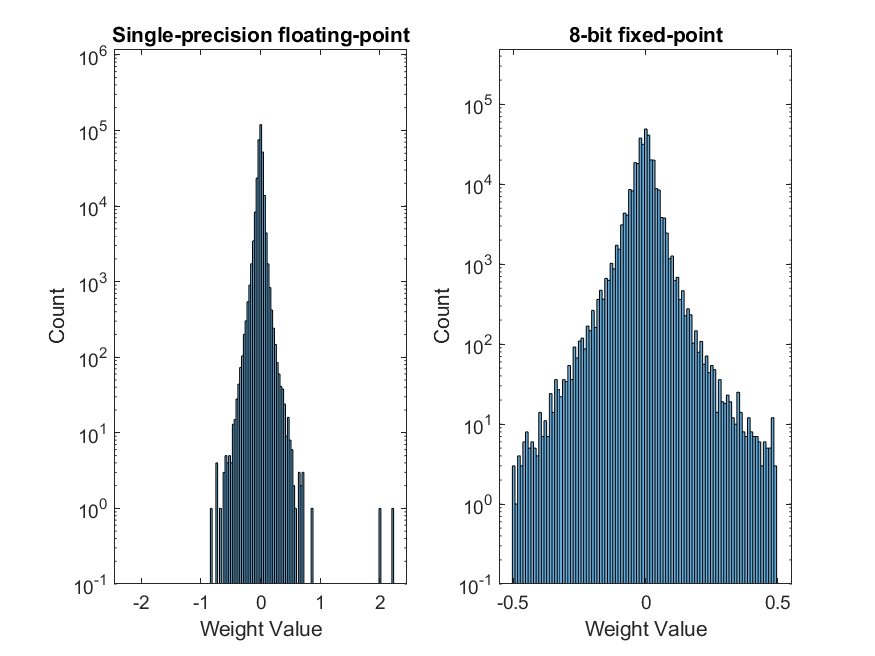
\includegraphics[scale=0.9]{Images/Weights-distributions/original-vs-fixed8/weight-distribution-conv2.png}
	\decoRule
	\caption[Second Convolution layer's weights distribution comparison between single-precision floating-point and 8-bit fixed-point representations]{Second Convolution layer's weights distribution comparison between single-precision floating-point and 8-bit fixed-point representations: right histogram's limits are significantly altered.}
	\label{fig:weight-distribution-comparison-conv2}
\end{figure}

This suppression is caused by the nature of the 8-bit fixed-point data type, which only allows 256 different values to be represented. Equation's \ref{eqn:select-radix-point-position} result is position 8, which means that the representation's step is $1/2^8 = 0.00390625$, hence its limits are $-2^7/2^8 = -0.5$ and $2^7/2^8 = 0.5$ (the most significant bit is used for the sign). Although there are some weights in the range of $(-2, -0.5) \cup (0.5, 2)$, their summed conversion accuracy error is less than the sum of accuracy errors of the smaller numbers, which are orders of magnitude more in count, when another radix-point position is selected. In other words, the sum of a lot of small errors is greater than the sum of a few big errors, causing the big errors the be ignored.

Second of all, figure \ref{fig:weight-distribution-comparison-conv5} depicts the fifth convolution layer's weights distributions of both their original single-precision floating-point and their 8-bit fixed-point converted representations. While this layer's weights distribution limits are not altered, various spikes on the right histogram can be observed.

\begin{figure} [H]
	\centering
	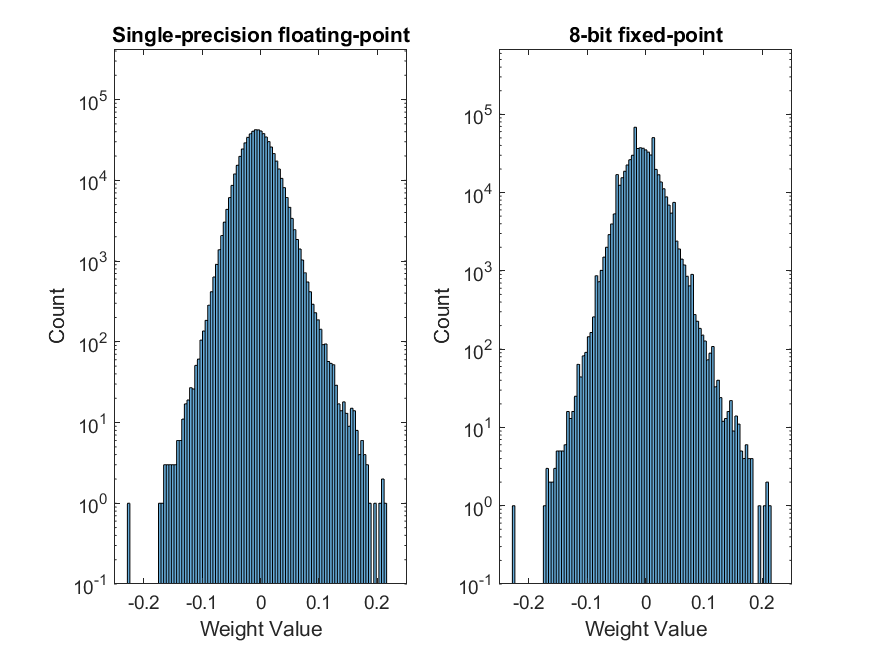
\includegraphics[scale=0.9]{Images/Weights-distributions/original-vs-fixed8/weight-distribution-conv5.png}
	\decoRule
	\caption[Fifth Convolution layer's weights distribution comparison between single-precision floating-point and 8-bit fixed-point representations]{Fifth Convolution layer's weights distribution comparison between single-precision floating-point and 8-bit fixed-point representations: various spikes can be observed on the right histogram.}
	\label{fig:weight-distribution-comparison-conv5}
\end{figure}

Those spikes are caused by the fixed-point's inability to represent all real numbers. It is the same reason the floating-point data type exists. The fifth convolution layer's radix-point is positioned on the 8th bit, which results in a representation step of $1/2^8 = 0.00390625$. This means that any weight with value ($i/8, (i + 1)/8)$, with $i=-2^7, -2^7 + 1, ..., 2^7$, is rounded to the nearest fixed-point number available. Therefore, many weights are rounded to their nearest fixed-point representation, creating those spikes, which is expected.

Last but not least, figure \ref{fig:weight-distribution-comparison-FC1} depicts the first Fully-Connected layer's weights distributions of both their original single-precision floating-point and their 8-bit fixed-point converted representations. In this figure's right histogram, a high amount of subsampling can be observed compared to the left one.

\begin{figure} [H]
	\centering
	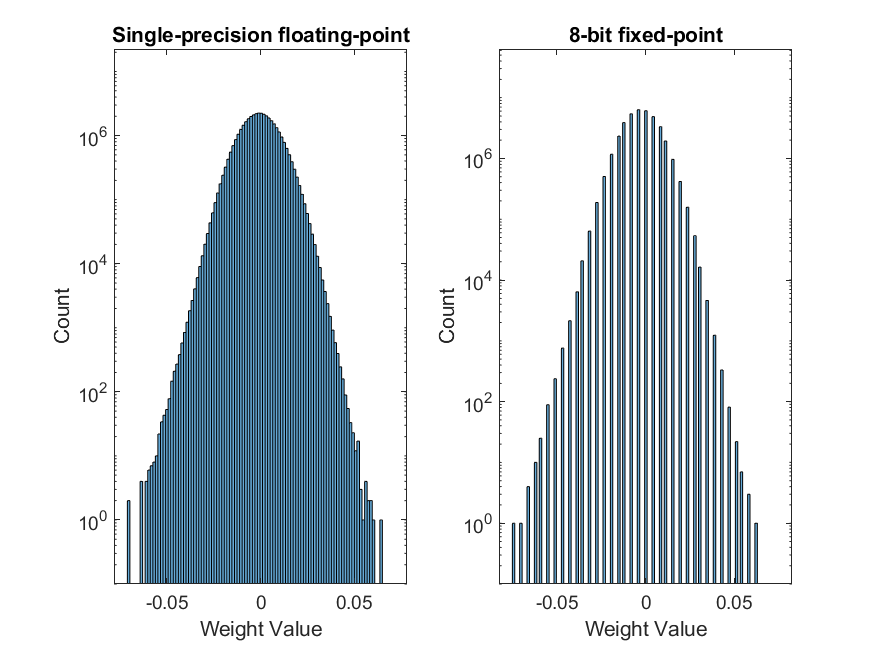
\includegraphics[scale=0.9]{Images/Weights-distributions/original-vs-fixed8/weight-distribution-FC1.png}
	\decoRule
	\caption[First Fully-Connected layer's weights distribution comparison between single-precision floating-point and 8-bit fixed-point representations]{First Fully-Connected layer's weights distribution comparison between single-precision floating-point and 8-bit fixed-point representations: significant subsampling on the right histogram.}
	\label{fig:weight-distribution-comparison-FC1}
\end{figure}

Again, this subsampling can be explained by the fixed-point's inability to represent all weights accurately, resulting in jumps. In this layer, equation \ref{eqn:select-radix-point-position} positioned the radix-point on the 8th bit, which, again, means a step of $1/2^8 = 0.00390625$.

To tackle with the suppression and subsampling side effects, an enhanced version of this technique was used. More specifically, instead of merely measuring the representation error of each weight and the summing it up with all other errors, as equation \ref{eqn:select-radix-point-position} does, it is essential to further amplify significant errors in order for them to stand out compared to the big count of small errors. This amplification can be done by adding non-linearity to the error's computation. The Mean Squared Error (MSE) can be used for this purpose, as shown in equation \ref{eqn:select-radix-point-position-Mean-Squared-Error}.

After observing the weights' distributions, it is clear that some distributions need a more accurate representation step. This is given by the radix point's position. So, instead of searching for a position on the given bit width, the radix-point should be allowed to exceed the number's bit-width. Therefore, the maximum radix-point was selected greedily to be 32.

\begin{equation}
	\label{eqn:select-radix-point-position-Mean-Squared-Error}
	Position = argmin_{i=0}^{32}[\frac{\sum_{j=1}^{size(S)} |S_j - FixPtConvert(S_j, W, i)|^2 }{size(S)}]
\end{equation}

Although equation \ref{eqn:select-radix-point-position-Mean-Squared-Error} resulted in better inference accuracy, after some experimentation, more amplification was needed to achieve the best accuracy possible with this technique. For AlexNet, the Mean Quarted Error (MQE), shown on equation \ref{eqn:select-radix-point-position-Mean-Quarted-Error}, yields the best results, and no further amplification is needed.

\begin{equation}
	\label{eqn:select-radix-point-position-Mean-Quarted-Error}
	Position = argmin_{i=0}^{32}[\frac{\sum_{j=1}^{size(S)} |S_j - FixPtConvert(S_j, W, i)|^4 }{size(S)}]
\end{equation}

As shown on figures \ref{fig:weight-distribution-comparison-conv2-MQE}, \ref{fig:weight-distribution-comparison-conv5-MQE} and \ref{fig:weight-distribution-comparison-FC1-MQE}, the suppression and the subsampling side effects are eliminated. There is still some spiking; however, it is expected behavior due to the lack of representation accuracy with fixed-point data types.

\begin{figure} [H]
	\centering
	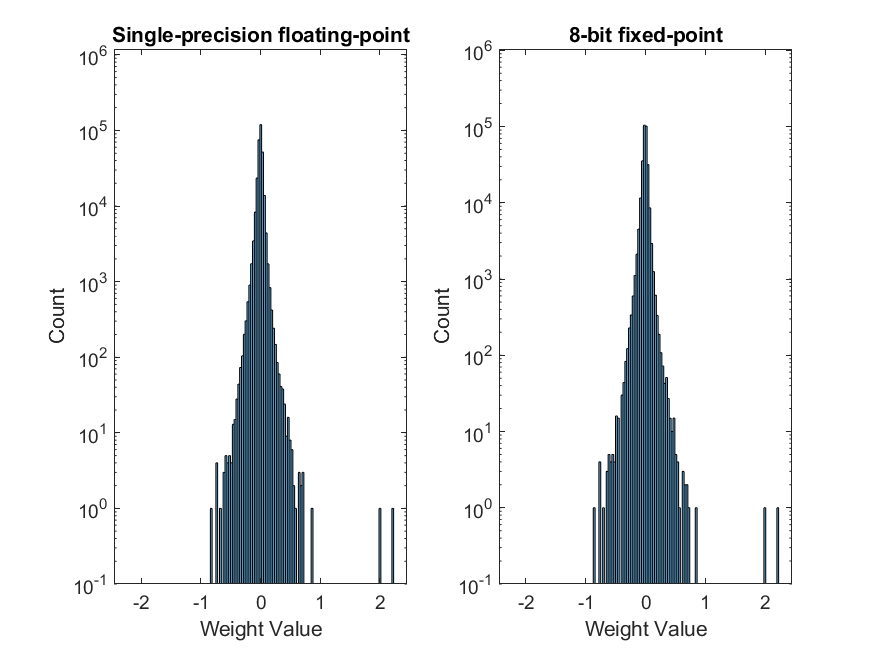
\includegraphics[scale=0.9]{Images/Weights-distributions/original-vs-fixed8/weight-distribution-conv2-MQE.png}
	\decoRule
	\caption[Second Convolution layer's weights distribution comparison between single-precision floating-point and 8-bit fixed-point representations using MQE]{Second Convolution layer's weights distribution comparison between single-precision floating-point and 8-bit fixed-point representations using MQE: right histogram's limits are identical.}
	\label{fig:weight-distribution-comparison-conv2-MQE}
\end{figure}

Using MQE, equation \ref{eqn:select-radix-point-position-Mean-Quarted-Error} resulted in the 5th radix-point position for the second convolution layer's weights. This results in a representation step of $1/2^5 = 0.03125$, hence its limits are $-2^7/2^5 = -4$ and $2^7/2^5 = 4$. Consequently, the whole weights range can be represented, removing the suppression problem.

\begin{figure} [H]
	\centering
	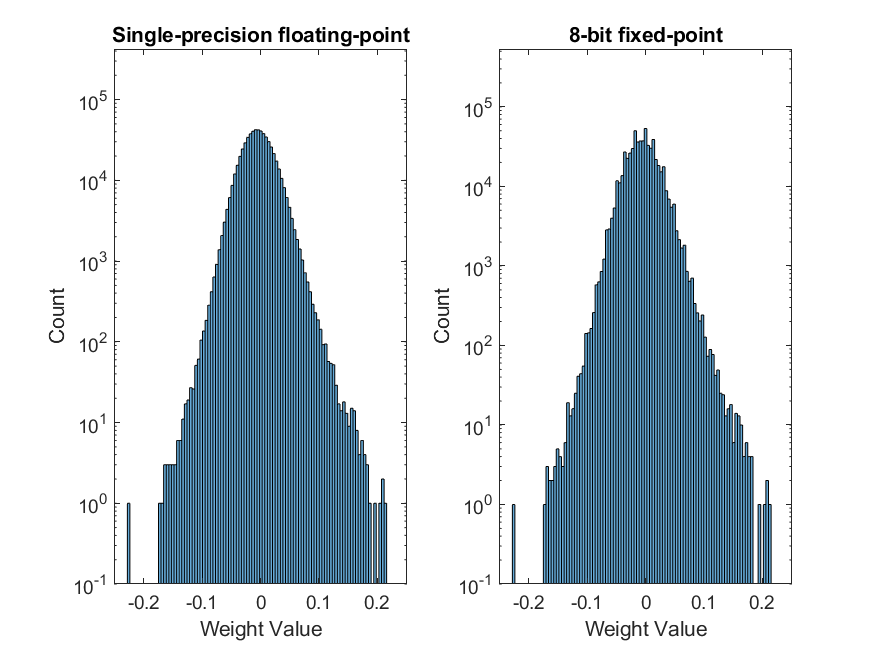
\includegraphics[scale=0.9]{Images/Weights-distributions/original-vs-fixed8/weight-distribution-conv5-MQE.png}
	\decoRule
	\caption[Fifth Convolution layer's weights distribution comparison between single-precision floating-point and 8-bit fixed-point representations using MQE]{Fifth Convolution layer's weights distribution comparison between single-precision floating-point and 8-bit fixed-point representations using MQE: various spikes can still be observed on the right histogram.}
	\label{fig:weight-distribution-comparison-conv5-MQE}
\end{figure}

Using MQE, equation \ref{eqn:select-radix-point-position-Mean-Quarted-Error} resulted in the 9th radix-point position for the fifth convolution layer's weights. This results in a representation step of $1/2^9 = 0.001953125$, hence its limits are $-2^7/2^9 = -0.25$ and $2^7/2^9 = 0.25$. Although, the spikes are not removed, there is a slight improvement in the weights representation accuracy.

\begin{figure} [H]
	\centering
	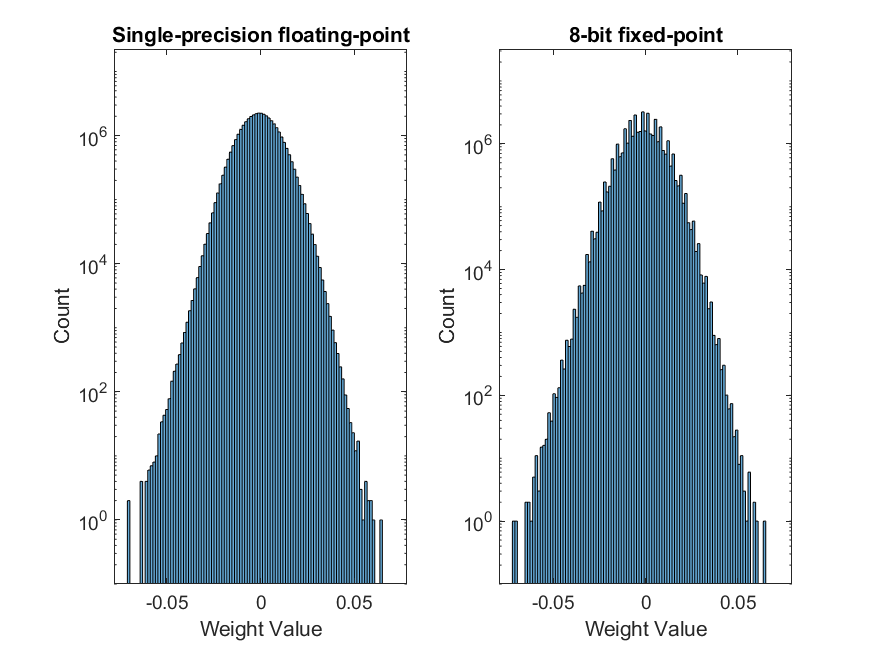
\includegraphics[scale=0.9]{Images/Weights-distributions/original-vs-fixed8/weight-distribution-FC1-MQE.png}
	\decoRule
	\caption[First Fully-Connected layer's weights distribution comparison between single-precision floating-point and 8-bit fixed-point representations using MQE]{First Fully-Connected layer's weights distribution comparison between single-precision floating-point and 8-bit fixed-point representations using MQE: no subsampling on the right histogram.}
	\label{fig:weight-distribution-comparison-FC1-MQE}
\end{figure}

Using MQE, equation \ref{eqn:select-radix-point-position-Mean-Quarted-Error} resulted in the 10th radix-point position for the first Fully-Connected layer's weights. This results in a representation step of $1/2^10 = 0.0009765625$, hence its limits are $-2^7/2^10 = -0.125$ and $2^7/2^10 = 0.125$. The added representation accuracy fully eliminates the subsampling problem, though some spiking is introduced as expected.

Table \ref{tab:fixed-MQE-error-rates} shows the Top-1 error-rate of fixed-point data types using the Mean Quarted Error equation \ref{eqn:select-radix-point-position-Mean-Quarted-Error}. While 8, 10, and 12 bit width fixed-point data types are still unusable, the 14 and 16 bit width representations have improved significantly.

\begin{table}[H]
	\caption{Top-1 error rate of fixed-point data types using Mean Quarted Error equation \ref{eqn:select-radix-point-position-Mean-Quarted-Error}.}
	\label{tab:fixed-MQE-error-rates}
	\centering
	\begin{tabular}{lll}
		\toprule
		\textbf{Tool} & \textbf{Data type} & \textbf{Top-1 Error rate (\%)}\\
		\midrule
			MATLAB 	& fixed64	& 0 	\\
			MATLAB 	& fixed32	& 0 	\\
			MATLAB 	& fixed16	& 4.42 	\\
			MATLAB 	& fixed14	& 17.59 \\
			MATLAB 	& fixed12	& 48.11 \\
			MATLAB 	& fixed10	& 86.91	\\
			MATLAB 	& fixed8	& 99.3 	\\
		\bottomrule\\
	\end{tabular}
\end{table}

For better clarity on the results, figure \ref{fig:data-types-accuracy-chart} depicts all tested data types and their Top-1 accuracy.

\begin{figure} [H]
	\centering
	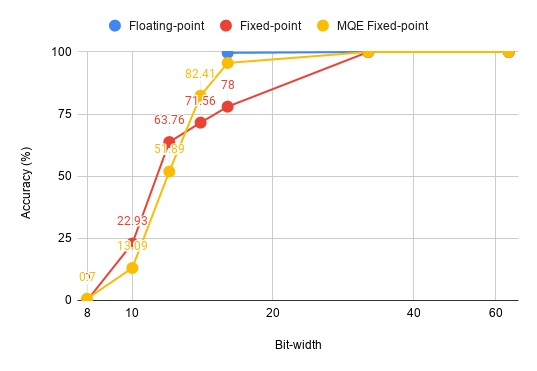
\includegraphics[width=\textwidth]{Images/Weights-distributions/data-types-accuracy-chart.png}
	\decoRule
	\caption[All data types tested accuracy]{All data types tested accuracy.}
	\label{fig:data-types-accuracy-chart}
\end{figure}

After some experimentation, dynamically assigning different bit-widths on each layer, according to its accuracy needs, rather than a single bit-width for the whole network, can yield even better results. However, further investigation has to be conducted.

\subsection{Fixed Point Activations}
Since floating-point arithmetic handles scaling automatically, the network does not face any overflow defects on its activations. However, when using fixed-point arithmetic, activations overflow is a severe problem. For instance, when multiplying 8-bit fixed point activations and weights, a new activation is generated with at most 16-bit width. Furthermore, adding two 16-bit activations can generate a new activation of 17-bit width. Therefore, if activations are not quantized between each layer, there will be a very wide output at the end of the network, wasting resources and performance when implemented in FPGAs.

Hence, between every layer, the activations should be quantized from their high-detail, large bit-width representations, back to some low bit wide representation. A question arises on how to quantize them in order to keep the most detail available. This work tries to keep the upper n bits from the first one. For example, let an activation implementation be 32-bit wide, its most significant one be on the 17th bit, and the new, low-detail representation be 8-bit wide. Then, if the upper 8 bits are kept, from the 31st bit down to the 24th bit, they will all be zeros, and as a result, its value will be lost. However, if the 8 bits from the first upper one are kept, from the 17th bit down to the 10th bit, the most significant detail is retained.

On the contrary, finding the most significant one on every activation in a single layer is not only computationally intensive but also requires that every activation has its own scale factor, rendering the fixed-point's benefits obsolete. All activations in a single layer should have the same scale factor, simplifying their arithmetic operations and minimizing required I/O.

Hence, an experiment was conducted to find each layer's optimal activation scale factor, whose results are depicted in table \ref{tab:Theoretical-and-Practical-activations-bit-widths}, using AlexNet as a reference. The theoretical bit-width represents the maximum bits needed to represent the layer's output adequately and can be calculated using equation \ref{eqn:theoretical-activation-bit-width}.
\begin{equation}
	\label{eqn:theoretical-activation-bit-width}
	Theoretical_{bitWidth} = input_{bitWidth} + weight_{bitWidth} + \lceil \log_2 \#Additions \rceil
\end{equation}

However, equation \ref{eqn:theoretical-activation-bit-width} calculates the maximum bit-width that could be generated after all operations, when all numbers are of max value, which is not the case. Therefore, the experiment includes a practical study of the maximum incurring bit-width, conducted by inferencing 2000 images and finding the maximum valued activation on each layer. Results of this experiment are depicted on column Practical bit-width of table \ref{tab:Theoretical-and-Practical-activations-bit-widths}.

\begin{table}[H]
	\caption{Theoretical and Practical activations' bit-widths}
	\label{tab:Theoretical-and-Practical-activations-bit-widths}
	\centering
	\begin{tabular}{lll}
		\toprule
		\textbf{Layer} & \textbf{Theoretical bit-width} & \textbf{Practical bit-width}\\
		\midrule
			Input & 8 & 8\\
			Conv1 & $ 8 + 8 + \lceil \log_2 3 * 11 * 11 \rceil = 25 $ & 17\\
			Conv2 & $ 8 + 8 + \lceil \log_2 64 * 5 * 5 \rceil = 27$ & 14\\
			Conv3 & $ 8 + 8 + \lceil \log_2 192 * 3 * 3 \rceil = 27$ & 15\\
			Conv4 & $ 8 + 8 + \lceil \log_2 384 * 3 * 3 \rceil = 28$ & 15\\
			Conv5 & $ 8 + 8 + \lceil \log_2 256 * 3 * 3 \rceil = 28$ & 17\\
			FC1 & $ 8 + 8 + \lceil \log_2 9216 \rceil = 30$ & 17\\
			FC2 & $ 8 + 8 + \lceil \log_2 4096 \rceil = 28$ & 17\\
			FC3 & $ 8 + 8 + \lceil \log_2 4096 \rceil = 28$ & 17\\
		\bottomrule\\
	\end{tabular}
\end{table}

As of table \ref{tab:Theoretical-and-Practical-activations-bit-widths}, the theoretical and practical bit-widths appear significant differences. Fortunately, the maximum theoretical bit-width is 30 bits, and consequently, all layers' activations can fit in 32-bit integer representations, before quantizing them.

The scale factor after the quantization of the layer's activations can be calculated using equation \ref{eqn:activations-scale-factor}, where $Practical_{bitWidth}$ is the activations' maximum practical bit-width as shown in table \ref{tab:Theoretical-and-Practical-activations-bit-widths} and $RepBits$ is the bit-width of the representation after the quantization.

\begin{equation}
	\label{eqn:activations-scale-factor}
	ScaleFactor = Practical_{bitWidth} - (\#RepBits - 1) + input_{scaleFactor} + weight_{scaleFactor}
\end{equation}

Table \ref{tab:Scale-Factor-per-layer} depicts the optimal scale factor for each layer's weights after their conversion from floating-point to 8-bit fixed-point as instructed by section \ref{sec:fixed-point}, and the scale factor of each layer's outputs.

\begin{table}[H]
	\caption{Scale Factor per layer}
	\label{tab:Scale-Factor-per-layer}
	\centering
	\begin{tabular}{lll}
		\toprule
		\textbf{Layer} & \textbf{Weights Optimal Scale Factor} & \textbf{Output Scale Factor}\\
		\midrule
			Input & -7 & -\\
			Conv1 & -5 & -2\\
			Conv2 & -5 & 0\\
			Conv3 & -5 & 3\\
			Conv4 & -6 & 5\\
			Conv5 & -5 & 10\\
			FC1 & -5 & 15\\
			FC2 & -6 & 19\\
			FC3 & -6 & 23\\
		\bottomrule\\
	\end{tabular}
\end{table}

\section{Weight Pruning}
Synaptic pruning is the biological brain's phase \cite{Synaptic-Pruning-Wikipedia}, during which both axons and dendrites of mammals brains decay and die off, typically occurring from the time of birth until the mid-20s on humans. Inspired by the Synaptic Pruning, Weight Pruning is a technique for artificial neural network compression, leading to smaller in size networks, higher memory and power efficiency, and faster inference times.

During the weight pruning procedure, the weights that contribute little or even nothing to the network's knowledge are getting pruned, or in other words, are getting zeroed out. This zeroing means that any activation multiplied by a zero weight also results in a zero. Hence, hardware accelerators can ignore zero weights and skip calculations, speeding up the overall inference procedure. In addition, more zeros also means higher compression rates of a layer's weights, and consequently, lower memory bandwidth requirements. However, similar to data type selection, weight pruning creates a tradeoff between inference performance and classification accuracy.

Also similar to the data type selection, the best weight pruning amount varies according to the network in question. Therefore, a specific investigation has to be conducted per network. For this work's reference network, AlexNet, a specific investigation has been conducted, whose results are shown on table \ref{tab:pruning-amount-vs-accuracy} and figure \ref{fig:pruning-amount-vs-accuracy}, the process of which is described below.

The weight pruning process requires a pruning factor \emph{f}, which will zero out every weight $w \epsilon [-f, f]$. Its selection is essential as it controls the pruning amount and the network's post-pruning accuracy. If the factor is too big, there might be a significant impact on accuracy, while if the factor is too small, then the compression might be ineffective.

A strategy for selecting the best pruning factor might be to use the same factor on all layers and measure the post-pruning accuracy. However, such a strategy leads to low accuracy on AlexNet. Since each AlexNet's layer weights distribution differs in variance, significant weights are valued differently. Figure \ref{fig:all-layer-original-weights-distributions} shows each AlexNet's layer weights distribution, making it clear that a global pruning factor cannot be used for high-performance rates; every layer has different limits on its weight distribution and different concentrations per weight value range.

A more suitable strategy would be to investigate a pruning factor for each layer. Starting from the first layer, prune its weights by some factor $f_1$, test the network for its accuracy. If accuracy results are not acceptable, repeat this step by selecting another value for $f_1$. If the accuracy is acceptable, continue to the second layer by selecting a new factor $f_2$. Test the network for classification accuracy with only the second layer's weight pruned by $f_2$. This process continues until the last layer, which in this work's network, AlexNet, is the third Fully-Connected layer. Finally, there will be the array $F = [f_1, f_2, ..., f_8]$ (for AlexNet), which includes all pruning factors, one per layer.

\begin{figure} [H]
	\centering
	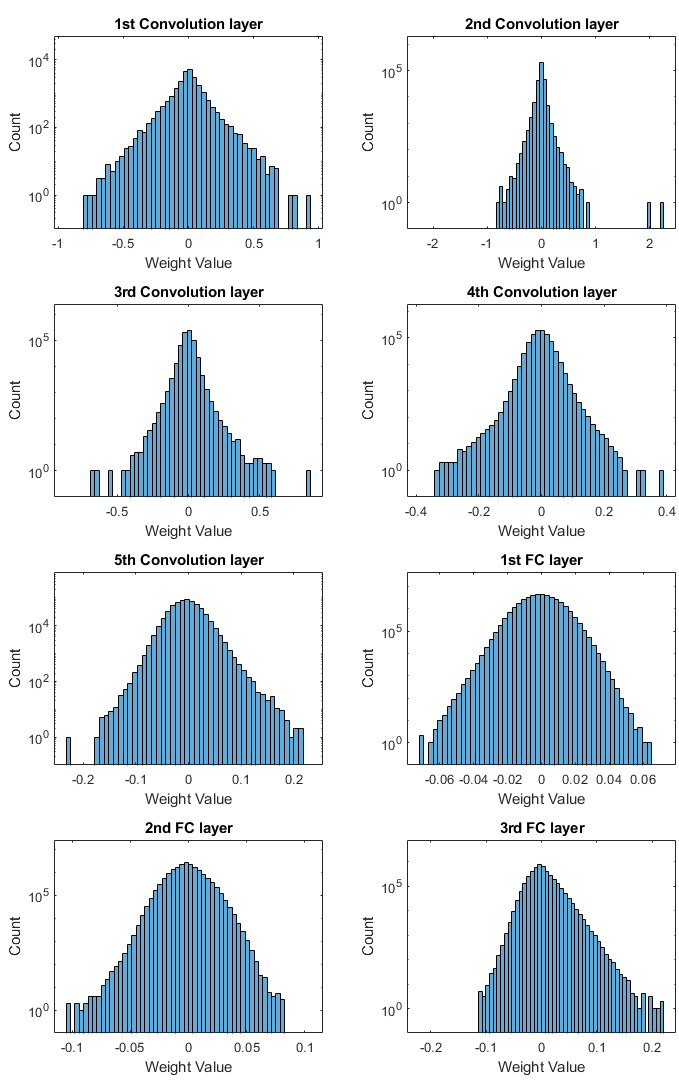
\includegraphics[width=\textwidth]{Images/Weights-distributions/all-layer-original-weights-distributions.png}
	\decoRule
	\caption[All layer weights distributions]{All layer weights distributions.}
	\label{fig:all-layer-original-weights-distributions}
\end{figure}

Table \ref{tab:pruning-amount-vs-accuracy} shows the weight pruning percentage per layer and all-layer total, with the classification accuracy yielded by each test. Seven tests are depicted, with different configurations each. Tests 1-4 use pruning on all layers, while tests 5-7 use pruning only on the Fully-Connected layers due to their enormous size (see table \ref{tab:AlexNet-Parameters-Memory-Footprint}).

Tests explanation:
\begin{itemize}
	\item \textbf{Test 1:} Low pruning amount on convolution layers, low pruning amount on Fully-Connected layers.
	\item \textbf{Test 2:} Medium pruning amount on convolution layers, low pruning amount on Fully-Connected layers.
	\item \textbf{Test 3:} High pruning amount on convolution layers, low pruning amount on Fully-Connected layers.
	\item \textbf{Test 4:} High pruning amount on convolution layers, high pruning amount on Fully-Connected layers.
	\item \textbf{Test 5:} No pruning on convolution layers, low pruning amount on Fully-Connected layers.
	\item \textbf{Test 6:} No pruning on convolution layers, medium pruning amount on Fully-Connected layers.
	\item \textbf{Test 7:} No pruning on convolution layers, high pruning amount on Fully-Connected layers.
\end{itemize}

\begin{table}[H]
	\caption{All pruning amount configurations tested and their accuracy.}
	\label{tab:pruning-amount-vs-accuracy}
	\centering
	\begin{tabular}{llll llll}
		\toprule
		\textbf{Layer} & \textbf{Test 1} & \textbf{Test 2} & \textbf{Test 3} & \textbf{Test 4} & \textbf{Test 5} & \textbf{Test 6} & \textbf{Test 7}\\
		\midrule
			Conv1 (\%) & 7.15 & 13.66 & 91.3 & 91.3 & 0 & 0 & 0 \\
			Conv2 (\%) & 13.82 & 26.9 & 95.83 & 95.83 & 0 & 0 & 0 \\
			Conv3 (\%) & 13.54 & 26.63 & 98.62 & 98.62 & 0 & 0 & 0 \\
			Conv4 (\%) & 15.32 & 29.99 & 93.14 & 93.14 & 0 & 0 & 0 \\
			Conv5 (\%) & 15.55 & 30.53 & 94.02 & 94.02 & 0 & 0 & 0 \\
			FC1 (\%) & 41.23 & 41.23 & 41.23 & 94.48 & 41.23 & 71.89 & 96.61 \\
			FC2 (\%) & 36.69 & 36.69 & 36.69 & 90.61 & 36.69 & 62.52 & 90.61 \\
			FC3 (\%) & 27.27 & 27.27 & 27.27 & 89.68 & 27.27 & 47.74 & 75.56 \\
			\midrule
			\textbf{Total (\%)} & 37.97	& 38.54 & 41.22 & 93.11 & 37.38 & 64.79 & 89.65 \\
			\midrule
			\textbf{Accuracy (\%)} & 91.74	& 80.8 & 0 & 0 & 90.87 & 71.77 & 15.06 \\
		\bottomrule\\
	\end{tabular}
\end{table}

From table \ref{tab:pruning-amount-vs-accuracy}, it is evident that increasing the pruning amount leads to lower accuracy. Test 1, which has the lowest pruning amount overall, yielded the best results. Similarly, concerning the tests 5-7, where only the Fully-Connected layers have been pruned, the test with the least amount of pruning, Test 5, resulted in the best accuracy. From the tests 1-4, one could argue that the convolution layers are more prone to error when increasing their pruning amount compared to Fully-Connected layers.

Tests 1 and 5 have identical pruning amount on the Fully-Connected layers; however, test 1 also uses pruning on convolution layers. While test 5 uses less pruning overall, it yields slightly lower accuracy compared to test 1. This could be explained because of the denoising characteristics that the weight pruning provides to the systems. Low and non-important weights could be characterized as noise, originating from the training procedure. Hence, cutting off the "noisy" weights could lead to higher accuracy, which is the case with tests 1 and 5.

Figure \ref{fig:pruning-amount-vs-accuracy} shows the two test groups' classification accuracy to total pruning amount. The first test group, tests 1-4, depicted with blue, is the one that all layers are getting pruned, while the second test group, test 5-7, depicted with red, is the one that only the Fully-Connected layers are getting pruned.

\begin{figure} [H]
	\centering
	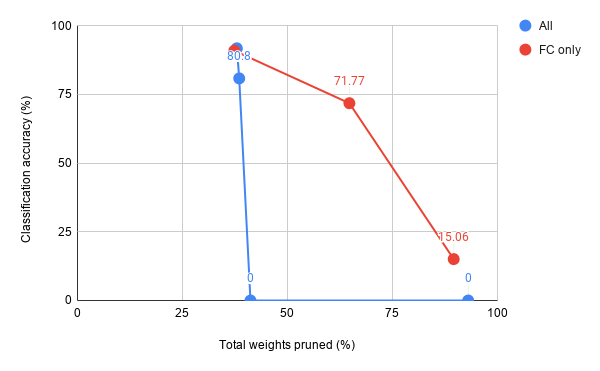
\includegraphics[width=\textwidth]{Images/Weights-distributions/pruned/pruning-amount-vs-accuracy-chart.png}
	\decoRule
	\caption[Accuracy per pruning amount]{Accuracy per pruning amount.}
	\label{fig:pruning-amount-vs-accuracy}
\end{figure}

It is obvious that pruning only the Fully-Connected layers has much potential and can lead to both high pruning amount and high classification accuracy. However, further investigation has to be conducted for the optimal pruning amount per layer on the whole network.

The effect of weight pruning can be clearly observed in figure \ref{fig:weight-distribution-comparison-pruned-conv1-test3}, which shows the original weight distribution of the first convolution layer (left) compared to the pruned weights distribution (right) of test 3.

\begin{figure} [H]
	\centering
	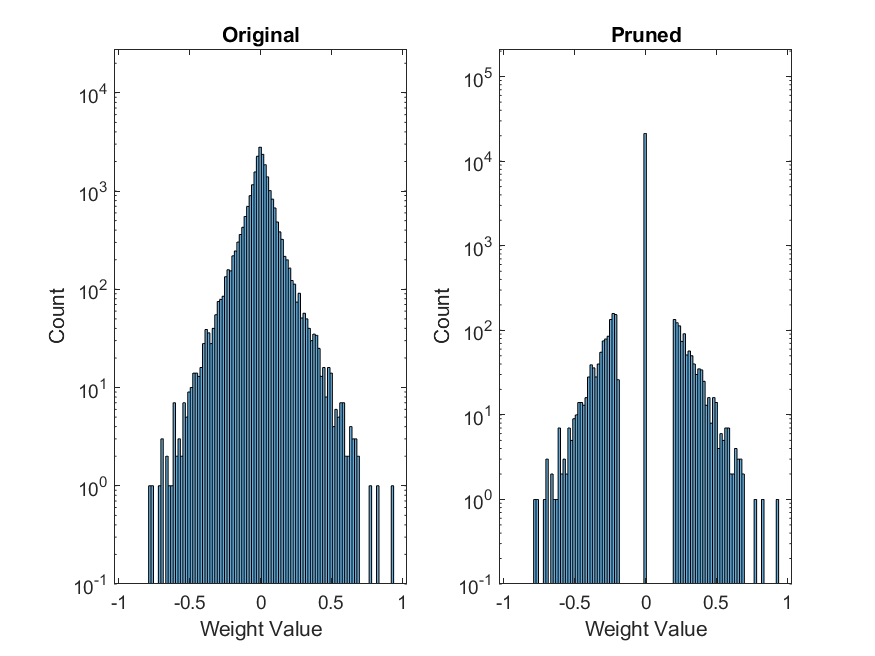
\includegraphics[width=\textwidth]{Images/Weights-distributions/pruned/41.22/weight-distribution-conv1.png}
	\decoRule
	\caption[Weight distribution comparison of the original and the pruned weights of the first convolution layer of test 3]{Weight distribution comparison of the original and the pruned weights of the first convolution layer  of test 3: A high concentration of zero valued weights can be observed on the pruned weights histogram (right), with a severe absence of near-to-zero valued weights.}
	\label{fig:weight-distribution-comparison-pruned-conv1-test3}
\end{figure}

A high concentration of zeros can be seen on the right histogram, combined with the absence of the near-to-zero valued weights ranging from -0.2 and 0.2. Similar are all layer's weight distributions of test 3, which uses aggressive pruning, creating severe alterations. The weights distributions discontinuity is responsible for the low classification accuracy.

Figures \ref{fig:weight-distribution-comparison-pruned-conv1-test1} and \ref{fig:weight-distribution-comparison-pruned-FC1-test1} demonstrate weight distributions of test 1, which yielded the best classifications overall tests. Those figures are an example of how a pruned distribution should look like to result in relatively high classification accuracy.

Figure \ref{fig:weight-distribution-comparison-pruned-conv1-test1} shows the weight distributions of the first convolution layer with the original and the pruned weights. No discontinuation can be observed on the pruned distribution, and similar to the original concentration of zero-valued weights.

\begin{figure} [H]
	\centering
	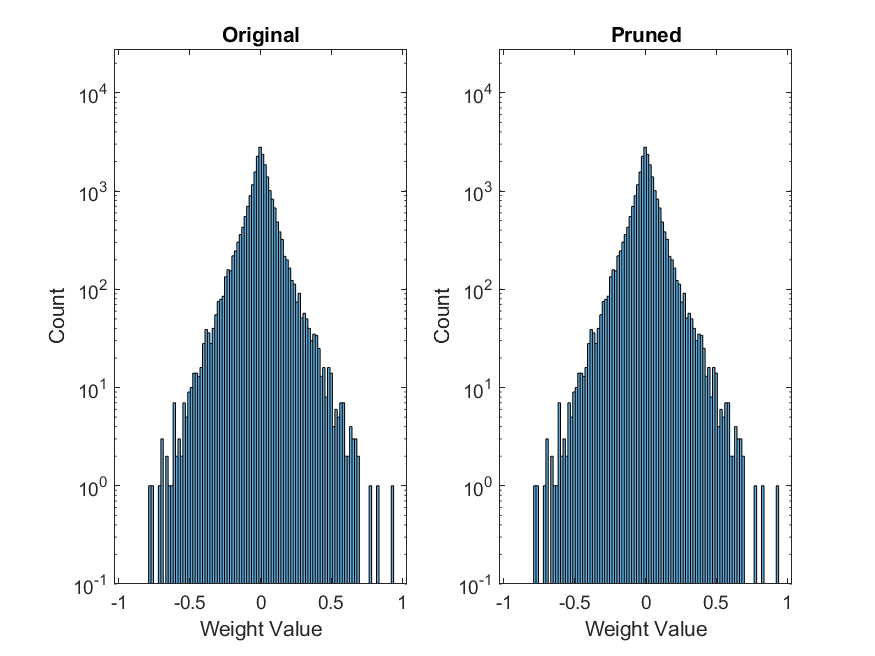
\includegraphics[width=\textwidth]{Images/Weights-distributions/pruned/37.97/weight-distribution-conv1.png}
	\decoRule
	\caption[Weight distribution comparison of the original and the pruned weights of the first convolution layer of test 1]{Weight distribution comparison of the original and the pruned weights of the first convolution layer of test 1: Similar concentration of zero valued weights can be observed on the pruned histogram (right), with almost no absence of near-to-zero valued weights.}
	\label{fig:weight-distribution-comparison-pruned-conv1-test1}
\end{figure}

Figure \ref{fig:weight-distribution-comparison-pruned-FC1-test1} shows the weight distributions of the first Fully-Connected layer with the original and the pruned weights. Slight discontinuation can be observed on the pruned distribution, with a higher concentration of zero-valued weights. It is vital that the discontinuation is kept really small.

\begin{figure} [H]
	\centering
	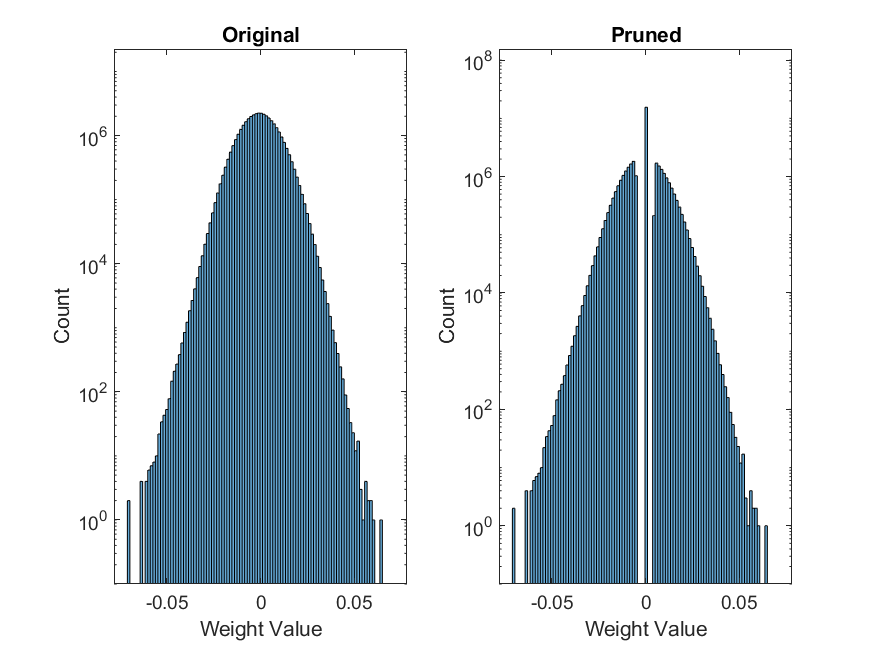
\includegraphics[width=\textwidth]{Images/Weights-distributions/pruned/37.97/weight-distribution-FC1.png}
	\decoRule
	\caption[Weight distribution comparison of the original and the pruned weights of the first Fully-Connected layer of test 1]{Weight distribution comparison of the original and the pruned weights of the first Fully-Connected layer of test 1: A high concentration of zero valued weights can be observed on the pruned weights histogram (right), with a slight absence of near-to-zero valued weights.}
	\label{fig:weight-distribution-comparison-pruned-FC1-test1}
\end{figure}

\chapter{FPGA Implementation}
\label{Chapter-FPGA-Implementation}

\section{Tools Used}
This work's CNN inference accelerator was implemented and optimized for FPGA platforms using the Xilinx Vivado Design Suite - HL System Edition 2019.2 \cite{Vivado-Design-Suite}. Vivado Design Suite is a software suite developed by Xilinx for its FPGA devices for analysis and synthesis of Hardware Description Language (HDL) designs, written in VHDL or Verilog. It is superseding Xilinx ISE \cite{Xilinx-ISE}, as a complete rewrite, with additional features for System-on-Chip (SoC) design and High-Level Synthesis (HLS). The tools used in this work are Xilinx Vivado HLS, Xilinx Vivado IDE, and Xilinx SDK.

\subsection{Vivado IDE}
Xilinx Vivado Integrated Design Environment (IDE), released in 2012, is the basis for all Xilinx tools. It serves as a GUI front-end for the Vivado Design Suite. All Vivado Design Suite tools integrate a native TCL interface, which can be accessed from IDE's GUI and the TCL console. Vivado IDE can compile, synthesize, implement, place and route FPGA hardware designs written in high-level languages such as C/C++, and HDLs such as VHDL and Verilog.

In addition, using the IP Integrator tool, hardware systems can be designed by graphically connecting IP blocks and configuring them through their GUI, with no coding involved, hence, accelerating the design process. Integration automation features such as auto-connecting and auto-configuring blocks further accelerate the design process. IP blocks can be created using the integrated IP Packaging functionality for VHDL or Verilog designs and via the Xilinx HLS tool for C/C++ designs. Xilinx also provides many IP blocks for free, including but not limited to on and off-chip-network IPs, memory blocks and memory management IPs, I/O interface IPs, and even various compute IPs. There are also additional IP's that can be purchased from Xilinx or even other vendors and developers.

After the design process is completed, a bitstream can be created and then downloaded to the target FPGA device to run as a standalone hardware device or in combination with firmware running on the FPGA's integrated ARM cores. The device's firmware is developed, compiled, and deployed using the Xilinx Software Development Kit (SDK) tool.

Designs can be tested on IP level or ever system-wide using the IDE's integrated simulator or any other RTL simulator. Moreover, Vivado IDE provides various debug tools that, combined with Integrated Logic Analyzer (ILA) IPs, can scan, check, and visualize the system's behavior during runtime.

\subsection{Vivado High-Level Synthesis (HLS)}
Xilinx Vivado High-Level Synthesis (HLS) \cite{Vivado-Design-Suite-User-Guide-High-Level-Synthesis}, currently rebranded as Xilinx Vitis HLS, is a tool included in the Xilinx Vivado Design Suite, allowing for a higher level of abstraction design of HDL systems. Vivado HLS synthesizes C/C++, SystemC and OpenCL functions into IP blocks, generating their VHDL and Verilog HDL designs that can then be implemented into hardware systems using Vivado and its Block Design tool.

While HLS accepts non-hardware-optimized code, it provides a set of directives that can instruct the synthesis procedure to implement a specific behavior, optimization, and resource management. Directives are optional and do not affect the input code's behavior. Their usage can both benefit the generated IP's performance and even hurt it when not used correctly. Furthermore, constraints, like clock period, clock uncertainty, and FPGA target, are added to the HLS synthesized IP blocks to ensure the desired behavior and performance.

A C/C++ testbench is used to debug the input code's behavior prior to synthesis, which should feed the input code with test data and check its output for correctness. Verification of the exported IP block is done using the C/RTL Cosimulation functionality, which uses the same C/C++ testbench, but replaces the function's call with the exported IP block call.

\subsubsection{Synthesis Report}
A synthesis report is created whenever HLS successfully synthesizes an IP Block, showing various performance and resource utilization metrics. Using the synthesis report, the designer can easily find and target the bottleneck to further optimize their design in terms of both performance and resources. Since Vitis HLS 2020.1, the report summary also contains the aforementioned information per loop per module, making the optimization procedure even more targeted. Some of the metrics are presented and explained below.

\begin{itemize}
	\item \textbf{Latency:} The number of clock cycles required for a complete run of a module or loop.
	\item \textbf{Iteration Latency:} The number of clock cycles required for running a single iteration of a module or loop.
	\item \textbf{Iteration/Initiation Interval (II):} The number of clock cycles required before a module can accept new input or a loop can initiate a new iteration.
	\item \textbf{Pipelined:} Whether a module or loop is implemented using a pipelined architecture.
	\item \textbf{Area:} The number of hardware resources a module requires for its implementation into the target FPGA. The hardware resource types are Block RAM (BRAM) and Ultra RAM (URAM), Digital Signal Processing (DSP) units, Flip Flops (FF), and Lookup Tables (LUT). A table is also given on the detailed report, showing the number of hardware resources required for every hardware component type, which include DSPs, Expressions, First-In-First-Out (FIFO) queues, Instances, Memories, Multiplexers, and Registers.
\end{itemize}

\subsubsection{Optimization Directives}
As mentioned above, HLS provides a set of directives for design optimization in terms of latency, throughput, and resource utilization of the exported IP block. Those directives can be added directly into the input code in the form of pragmas that the preprocessor can read. Another way of adding directives is by creating a new solution and automatically adding them to it. Every solution combines a set of directives and configurations into TCL files, one TCL file per solution. Multiple solutions can be created, each with different directive combinations and configurations. This way allows for better experimentation and fine-tuning of the design. Some optimization directives are presented and explained below.

\begin{itemize}
	\item \textbf{Interface:} The top-level function's arguments have to be mapped to RTL ports to configure the IP block's functionality. The interface directive specifies each argument's port type.
	\item \textbf{Stream:} By default, the top-level function's array arguments are implemented as RAM channels. However, when data are being produced or consumed sequentially, a more efficient data type is to use FIFOs, which can be specified using the stream directive.
	\item \textbf{Pipeline:} Given an \emph{Initiation Interval (II)} parameter, the pipeline directive reduces the number of clock cycles a function or loop can accept new inputs, targeting \emph{II} clock cycles, by allowing the overlapped execution of operations.
	\item \textbf{Unroll:} Given a \emph{factor}, the unroll directive unrolls a loop \emph{factor} times, creating multiple instances of the loop body, that can then be scheduled independently or run in parallel.
	\item \textbf{Loop Flatten:} Allows perfectly nested loops, loops that no logic is injected between them, to get collapsed into a single loop, reducing latency. Essentially, it handles all the indexing logic of the loop flattening.
	\item \textbf{Loop Merge:} Merges consecutive loops, often initialization loops, reducing overall latency and resource utilization.
	\item \textbf{Resource:} Specifies the resource for a variable to get implemented.
	\item \textbf{Array Partition:} By default, every array is implemented as a set of at least one BRAM unit with a single read and a single write port. The array partition directive partitions an array into multiple smaller arrays or assigns each array's element to its register. This partitioning increases the read and write ports of the array on the hardware level, allowing for parallel I/O and computations. In the potential expense of more memory instances and more register, array partitioning can improve overall throughput and performance of memory bounded applications.
	\item \textbf{Array Map:} The array map directive combines multiple small arrays into a single large one, to avoid BRAM waste on small arrays, which can occupy a BRAN unit for just a few elements.
	\item \textbf{Array Reshape:} Reshapes an array of many elements of small bit-width to an array of fewer elements but of higher bit-width, increasing the sequential BRAM access speeds.
	\item \textbf{Data Pack:} Similar to the array reshape directive, the data pack directive combines struct data fields to a single scalar of higher bit-width.
	\item \textbf{Dataflow:} Enables parallel execution of functions and loops, increasing throughput and latency.
	\item \textbf{Inline:} Similar to C/C++ macro preprocessor functionality, the inline directive injects a function's body to each of its calls, reducing latency and initiation interval due to lower function call overhead.
	\item \textbf{Allocation:} Limits the number of hardware resources used for implementing the IP block, and may result in hardware sharing and latency increase.
	\item \textbf{Latency:} Limits the minimum and maximum latency in clock cycles.
\end{itemize}

\subsection{Xilinx SDK and Xilinx Vitis IDE}
Xilinx Software Development Kit (SDK) \cite{Xilinx-SDK}, currently unified with SDSoC and SDAccel into Vitis Unified Software Platform, is an IDE for embedded-software development Xilinx's microprocessors. Based on the Eclipse IDE \cite{Eclipse-IDE}, it includes a C/C++ editor, a compilation toolchain for ARM microprocessors with automatic Makefile generation, system performance analysis and optimization tools, and several debug and profiling tools. It is used to create applications that run on the ARM cores either external to the FPGA die or internal like on the MPSoCs. Often those applications play the role of the coordinator/master that organizes, schedules, and configures the FPGA hardware. They often handle the external I/O, like data transfers to and from storage devices (SD cards, Hard Drives, Flash Memories, etc.) or Ethernet, to and from volatile memory (RAM, BRAM, etc.). They can also handle the data pre-processing needed to feed the FPGA hardware. Furthermore, multi-core processors can be utilized simultaneously using bare-metal applications. If multi-processing is required with a sophisticated scheduler, Linux applications can be built and run on Linux operating systems like PetaLinux \cite{PetaLinux} and FreeRTOS \cite{FreeRTOS}.

Xilinx SDK is strongly coupled with the Xilinx Design Suite and its hardware designs and bitstreams. After the successful implementation and bitstream generation of the hardware design from Vivado IDE, Xilinx SDK imports the project's hardware wrapper to generate the Board Support Package (BSP) and various C/C++ libraries useful for communication with and configuration of the FPGA hardware.

Xilinx SDK can create three main types of applications; bare-metal, First Stage Boot Loader (FSBL), and Linux applications. Their main difference is on the way the application is loaded onto the system's processor.
\begin{itemize}
	\item \textbf{Baremetal:} A bare-metal application is loaded using the SDK's built-in functionality that can program the FPGA (PL part) and load it onto the corresponding ARM core through the JTAG port.
	\item \textbf{FSBL:} A FSBL application is a set of files generated by the SDK that, when put on the root folder of the system's primary storage device, e.g., SD card, are read during the system's boot-up, triggering a boot loader sequence. The system has to be appropriately configured, typically configuring some jumpers and switches on development boards to instruct the processor to read the FSBL files. When the bootloader sequence is triggered, programming of the FPGA and loading the application are done using the primary storage device as a source, with no need for an external computer, and Xilinx SDK or JTAG.
	\item \textbf{Linux:} A Linux application is similar to the FSBL one, with the only difference that a Linux operating system is required to be running on the system's processor. Similarly, the Linux OS is loaded using the primary storage device. When Linux is fully loaded, the application can be started like any other Linux application through the provided console window to program the FPGA and run it.
\end{itemize}
A console window is used for input and output functionality using the UART port in all application types.

Debugging applications is as simple as regular locally running applications using the built-in System Debugger or other debugging tools like GDB \cite{GDB}. In addition, Vivado IDE's Hardware Manager can be used in combination with SDK's System Debugger to debug hardware designs and their driver applications. Vivado IDE's Hardware Manager connects to the hardware's ILA IPs, enabling the monitoring in real-time of the hardware's state concerning the driver application's state.

\section{FPGA Platforms}
\label{sec:FPGA-Platforms}
This work focuses on the two FPGA platforms available in the lab, the Xilinx ZCU102 Evaluation Kit, and the FORTH QFDB. Conveniently, both platforms integrate the same Zynq UltraScale+ MPSoC XCZU9EG-2FFVB1156E.

\subsection{Xilinx Zynq UltraScale+ MPSoC XCZU9EG-2FFVB1156E}
The Xilinx Zynq UltraScale+ Multi-Processor System-on-Chip (MPSoC) \cite{DS891-Zynq-UltraScale-MPSoC-DataSheet-Overview} family of products integrates multiple ARM Cortex-A53 and Cortex-R5 cores processing system (PS) and a Xilinx UltraScale programmable logic (PL) architecture in a single chip with on-chip memory, multiport external memory interfaces and several peripheral connectivity interfaces.

Some key features of XCZU9EG-2FFVB1156E are:
\begin{itemize}
	\item Quad-core 64bit ARM v8-A Cortex-A53 with L1/L2 cache.
	\item Dual-core 32bit ARM v7-R Cortex-R5 with L1 cache.
	\item ARM Mali-400 MP2 graphic processing unit.
	\item 256KB on-chip ECC memory.
	\item Xilinx 16nm FinFet+ programmable logic fabric.
	\item 600k system logic cells.
	\item 548k CLB Flip-Flops.
	\item 274k CLB LUTs.
	\item 32.1Mb Block RAM.
	\item 2520 DSPs.
\end{itemize}

\subsection{Xilinx ZCU102 Evaluation Kit}
The Xilinx ZCU102 Evaluation Kit \cite{ZCU102-User-Guide} \cite{ZCU102-Product-Overview} (Figure \ref{fig:ZCU102-board-overview}) is a general-purpose development board for rapid prototyping based on the aforementioned UltraScale+ MPSoC. It provides a complete platform with an SD card as a primary storage device, 4GB 64bit ECC DDR4 SODIMM RAM, 512MB DDR4 component memory for PL, and a power delivery system. It also provides various configuration switches and jumpers, and all major peripherals and interfaces such as PCIe Gen 2x4 slot, SATA, Ethernet, HDMI input and output, DisplayPort, USB, JTAG, and UART.

\begin{figure} [H]
	\centering
	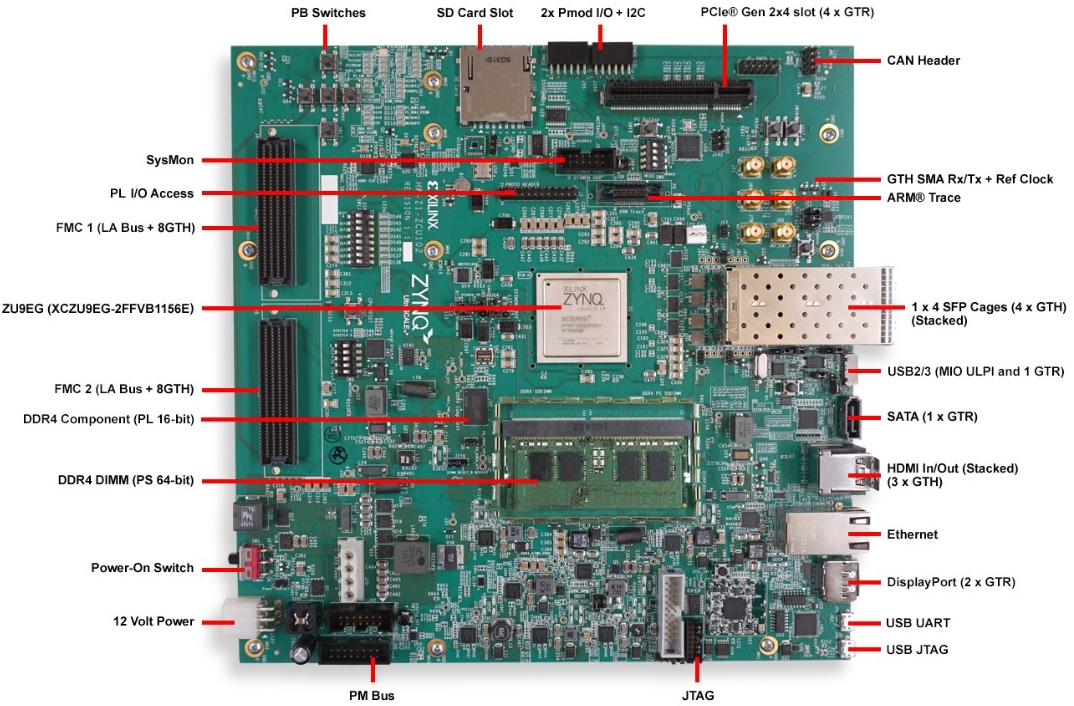
\includegraphics[width=\textwidth]{Images/Hardware/ZCU102-board-overview.jpg}
	\decoRule
	\caption[Xilinx ZCU102 Evaluation Board overview]{Xilinx ZCU102 Evaluation Board overview: \href{https://www.xilinx.com/products/boards-and-kits/ek-u1-zcu102-g.html}{URL}}
	\label{fig:ZCU102-board-overview}
\end{figure}

\subsection{FORTH QFDB}
The Quad-FPGA Daughter Board (QFDB) (Figure \ref{fig:forth-qfdb-daughterboard}) \cite{Implementation-and-Impact-of-an-Ultra-Compact-Multi-FPGA-Board-for-Large-System-Prototyping}, developed by the Foundation of Research and Technology Hellas (FORTH) \cite{FORTH}, combines four of the aforementioned MPSoCs, interconnected with each other. It is a complete platform as well, which provides 16GB of DDR4 memory and an M.2 Solid State Drive (SSD), and some peripherals and interfaces such as Ethernet, JTAG, and UART.

It is designed to be used in servers, with other QFDBs running in parallel, creating a network of FPGAs. The QFDB enables massive hardware designs to be split and deployed into multiple FPGA devices or even multiple QFDB boards. It also enables the deployment of hardware designs into a high number of FPGAs for increased parallelism.

\section{The Platform}
For this work, a platform was created capable of CNN inference on FPGA devices. This platform had to be created with flexibility and versatility in mind to be able to be transferred to other FPGA devices while being based on the Xilinx ZCU102, which was available in the lab. It should also be scalable to enable multi-FPGA implementations, and it should be extendable to enable for easy adding of new layer types and new layer accelerators. Furthermore, it should be able to run various CNN models' inference, but most importantly, it should provide easy experimentation and development of hardware accelerator architectures.

The basic building blocks of this platform consists of its volatile and non-volatile memory, and its compute engine. Figure \ref{fig:platform-block-diagram} depicts the platform's block diagram, whose functionality is explained below. It should be noted that everything described below is implemented on the aforementioned Xilinx ZCU102 Evaluation Kit.

\begin{figure} [H]
	\centering
	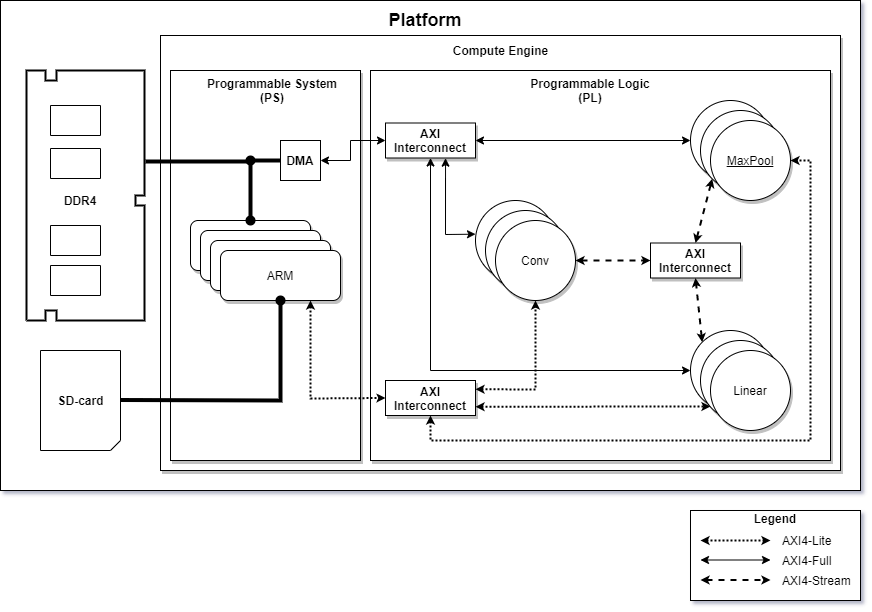
\includegraphics[width=\textwidth]{Images/Platform/platform.png}
	\decoRule
	\caption[The platform's block diagram]{The platform's block diagram.}
	\label{fig:platform-block-diagram}
\end{figure}

\subsection{Non-Volatile Memory}
This platform's non-volatile memory serves as a storage medium for all the data that networks require for their inference, which include the initialization data (network model configurations, parameters (weights and biases), class labels), and the input data (e.g., images). An SD-card is used as the non-volatile memory for this platform (also depicted as an SD-card in Figure \ref{fig:platform-block-diagram}). However, with some software extensions, other storage devices can also be used, such as SATA hard drives or even M.2 SSDs (on other FPGA platforms, e.g., QFDB). Moreover, external storage devices can also be utilized, via the Ethernet port through local-network/Internet, or via the JTAG port to avoid copying files over and over again on the platform's primary storage device but also to enable the single-source access for multiple FPGA devices.

While SD-cards have little bandwidth than other storage devices like SATA drives and M.2 SSDs, the non-volatile memory's purpose is to initialize the platform, which is a one time cost, and feed it with input data. When the platform is on its initialization phase, the initialization data from its non-volatile memory are transferred to its volatile memory to get later used from the compute engine. Because most, if not all, networks' initialization data fit in the volatile memory, leaving a lot of empty memory space, input data are also transferred, filling as much space as possible to utilize the volatile memory's high bandwidth for input data consumption. Consequently, the SD-card's low bandwidth can be safely ignored.

If the input data are large enough to not completely fit in the volatile memory and their consumption is faster than their feed through the SD-card, a faster storage device should be used. However, in this work's experiments, this has never been the case.

\subsection{Volatile Memory}
The platform's volatile memory consists of two types of memory devices, the DDR4 modules found on the ZCU102 and the on-chip BRAM. The ZCU102 also provides a separate DDR4 component accessible from the FPGA's PL part, however for simplicity and generality (it is not provided on all FPGA platforms) purposes, and because it provides lower bandwidth compared to the DDR4 modules, it is not utilized on this platform.

The platform's primary memory medium is the DDR4 memory modules  (also depicted as a DDR4 module in Figure \ref{fig:platform-block-diagram}) connected to both the PS and PL parts of the device. As mentioned before, it stores and serves all the required data for the platform to run. Those data are read from various files found on the non-volatile memory, in this case, the SD-card, using the ARM cores found on the PS part, and are then stored onto the DDR.

The DDR has to feed the PL part with data in chunks because, as explained in section \ref{sec:Memory-Footprint}, the integrated BRAM cannot store the whole network's parameters and activations. Consequently, every network's layer has to know where to find and how to access every piece of data it requires, information that is found on the platform's software structures and passed to the layers using the ARM cores during the setup phase.

On this platform, there is no central BRAM component that every accelerator accesses. Instead, every accelerator should implement its own BRAM, without permitting access to others. It should be the only one to know how to manage its storage. Of course, to fulfill the accelerator's needs in bandwidth, read and write ports, and latency, it can implement its BRAM as it requires, and utilize individual registers.

\subsection{Compute Engine}
The compute engine consists of both the PS and PL part of the FPGA device, which includes the ARM cores and the FPGA accelerators, respectively. While the bulk of the computation is handled by the PL part, the PS part handles the more sophisticated computations, such as the input data pre-processing and the accelerator configuration and scheduling.

In this platform, a network can be run only if its layers are supported by either software or hardware implementations. Software implementations are running on the ARM cores, and hardware implementations are the FPGA accelerators. By allowing both types of implementations, this platform expands its flexibility. This can not only help the development stage of FPGA accelerators by comparing their outputs with the ones generated by the software implementation, but it can also help to fully utilize the device's resources by running parts of even whole layers on the ARM cores in parallel to the hardware accelerators. Furthermore, layers that have not yet been implemented in hardware can easily be implemented in software for experimentation purposes, such as the Depth Concat layer found on the GoogLeNet (Figure \ref{fig:GoogLeNet}).

As shown in Figure \ref{fig:platform-block-diagram}, in this work, three layer types have been implemented in hardware; the Convolutional (Conv) layer, the Max-Pooling (MaxPool) layer and the Fully-Connected (Linear) layer. In addition, multiple instances of the same layer type can also be added in the platform to enable for either parallel execution of different inferences with different inputs or even different network models, or better pipelining in a single inference. This is discussed in detail in section \ref{sec:CNN-Scheduling}.

In this work, every accelerator implements a layer type, and, therefore, the platform assumes that every accelerator can handle and compute a whole layer type's computation. Every accelerator comes with its driver, which is integrated into the platform's software. The driver is responsible for setting up its accelerator, which includes setting the layer's hyperparameters and passing the information of where to find its parameters (weights and biases), its input data, and where to send its output data. Also, the driver handles the accelerator's interrupts, which,  in this work, only includes the accelerator completion interrupt.

The assumption that every accelerator implements a whole layer type simplifies the accelerator's driver. As a result, the driver does not have to know its accelerator's inner workings and architecture, except for its aforementioned settings, treating it as a black box with inputs and outputs. However, those settings are the same for every implementation of the same layer type; hence, experimenting with different architectures is made easy without developing a different driver for every single architecture. The driver can be reused on the same layer type accelerators, letting the engineer focus their efforts on the accelerator's architecture. Of course, every different layer type needs different settings; therefore, different drivers.

It is worth mentioning that every accelerator has an AXI4-Lite \cite{UG1037-Vivado-Design-Suite-AXI-Reference-Guide} slave port through which it can get configured. All accelerators' AXI4-Lite slave ports are connected to a Xilinx AXI SmartConnect IP \cite{PG247-SmartConnect-Product-Guide}, onto its master ports. The AXI SmartConnect, a replacement of the AXI Interconnect IP, acts as a router, providing a single slave port that is finally connected to the Zynq's (ARM cores) master port. AXI SmartConnect automatically detects the port's protocol, in this case, AXI4-Lite, and adjusts its ports accordingly. This creates a hardware connection so that the software can access and configure the platform's accelerators. Details on the AXI protocol are given in section \ref{sec:AMBA-AXI4-Interface-Protocol}.

\subsection{I/O}
\label{sec:IO}
As explained in previous sections, the I/O bandwidth provided to any hardware platform plays an essential role in its performance due to the CNNs' high bandwidth requirements. Hence, the platform should implement a network for its accelerators to enable the communication between them, the PS part, the DDR, and each other. There are three ways for high bandwidth communication, which are discussed below.
\begin{itemize}
	\item \textbf{Memory-Mapped I/O (MMIO):} In this method, the PS communicates with its PL part's accelerators using a global address space for both its main memory (DDR) and the accelerators' I/O extensions, mapping every memory component, such as the DDR, BRAM, and registers, onto its own address range. While it is straightforward to implement, it can create a bottleneck on random memory accesses onto the DDR, with each request costing up to 50 clock cycles for the DDR's initialization. Fortunately, this is not the case with burst accesses, which request only once a range of addresses so that there is only one initialization cost for a big transfer of data.
	\item \textbf{Streaming (AXI4-Stream):} Using streaming interfaces, such as the AXI4-Stream, continuous communication can be established between components in a FIFO manner. Every streaming connection creates a channel between the two components with a predefined FIFO size, with a producer-consumer behavior. Communication between hardware accelerators and the DDR can be established using the Xilinx AXI DMA IP \cite{PG021-AXI-DMA-Product-Guide}, which hides the DDR's initialization costs. However, AXI DMA requires knowledge of the data flow, and its function is instructed by the PS part for every transfer, increasing the system's complexity.
	\item \textbf{BRAM:} This method is an MMIO variation, which uses BRAM IPs to store the required data on-chip, taking advantage of the BRAM's high bandwidth. Data are transferred from the DDR to the BRAM in bursts using a Xilinx CDMA IP \cite{PG034-AXI-Central-Direct-Memory-Access-Product-Guide} connected to a Xilinx BRAM Controller IP \cite{PG078-AXI-BRAM-Controller-Product-Guide} and its Xilinx Block Memory Generator IP \cite{PG058-Block-Memory-Generator-Product-Guide}. Though, a major constraint is that the data have to be small enough to fit into the chip's BRAM, which is in the order of a few MBs in size.
\end{itemize}

As explained in section \ref{sec:Memory-Footprint}, the integrated BRAM cannot store the parameters for most layers. There is the case that parameters can be transferred in chunks to the central Block Memory IP; however, this creates further complexity and bandwidth bottleneck due to the low number of read and write ports. Therefore, the BRAM method described above cannot be used in this platform.

Hence, the question that arises is which method is more suitable for this platform, the MMIO or the Streaming one. To answer it, a test system was created, integrating a simple IP, created using Vivado HLS, that adds a specific value to its input data, and then returns its output data. The input data are generated on the PS part and are stored on the system's DDR. The IP's output is returned to the PS part and stored on its DDR. Then the PS validates the outputs to ensure their correctness. The IP's input and output ports are implemented both as streams and as MMIO.

The test measures the average number of clock cycles it takes for both implementations to process 40MB of data in chunks of 40kB. The chunk's size was selected greedily, because most, if not all, accelerators' requests need to be at least 40kB. The time measurement includes the input data transfer from the DDR to the IP's BRAM, the input data processing, and the output data transfer from the IP's BRAM to the system's DDR. Both implementations were tested with 32 and 128 input and output ports bit-width. The test's results are shown on table \ref{tab:MMIO-vs-Stream}.

\begin{table}[H]
	\caption[MMIO vs Stream]{MMIO vs Stream: Processing 40MB data of 40KB bursts, showing a slight advantage over the MMIO method.}
	\label{tab:MMIO-vs-Stream}
	\centering
	\begin{tabular}{lll}
		\toprule
		\textbf{Port bit-width} & \textbf{MMIO avg. cycles} & \textbf{Streaming avg. cycles}\\
		\midrule
			32-bit 	& 62700922 & 65611580\\
			128-bit & 15761270 & 16201797\\
		\bottomrule\\
	\end{tabular}
\end{table}

Both implementations for both port bit-widths show similar results, with a slight advantage over the MMIO implementation. Selecting MMIO for the primary method of data feeding the accelerators benefits the platform not only in terms of bandwidth, according to the slight advantage depicted on table \ref{tab:MMIO-vs-Stream}, but also in terms of simplicity of both software and hardware implementation and efficiency of hardware resources.

Consequently, the connection between the accelerators and the PS part and its DDR is established using the MMIO method, as shown on the platform's block diagram (Figure \ref{fig:platform-block-diagram}). Every accelerator has an AXI4-Full \cite{UG1037-Vivado-Design-Suite-AXI-Reference-Guide} master port, which is connected to a Xilinx AXI SmartConnect IP, onto its slave ports. The SmartConnect's master port then gets connected onto the Zynq's slave port. Communication to the DDR is established via the Zynq's slave port, and an integrated DMA found on the PS part.

However, the streaming method cannot be dismissed entirely, as it is perfect for communication between accelerators. Passing a layer's activations to its next layer, in terms of hardware means passing the accelerator's output data to the next accelerator as input data. Implementing this data transfer in a streaming manner avoids transferring data from the FPGA to the DDR and then transferring them back to the FPGA using the MMIO method, which can be a significant bottleneck. As a result, every accelerator can optionally have additional input stream and output stream ports. The accelerators driver configures it to either use the MMIO or the streaming method.

It is vital that every accelerator implements at least the MMIO method, to avoid running into deadlocks. For example, let there be a system with one instance of a layer type's accelerator, and the accelerator's output stream needs to get connected back to the same accelerator's input stream. A deadlock occurs when the output stream is full while the accelerator has not finished its execution. In this case, the accelerator hangs, waiting for the stream to accept more data, while the stream hangs, waiting for its data to get consumed. This problem can easily be tackled by simply sending the accelerator's outputs to the DDR using the MMIO method, and when its execution is complete, it can then read them back again from the DDR.

A Xilinx AXI4-Stream Switch IP \cite{PG085-AXI4-Stream-Infrastructure-IP-Suite-Product-Guide} is used to create a star topology \cite{Network-Topology-Wikipedia} stream network, connecting every accelerator's stream ports, as shown on the platform's block diagram (Figure \ref{fig:platform-block-diagram}). Every connection is assigned an address in the AXI4-Stream Switch IP before synthesis so that the TDEST signal of the AXI4-Stream protocol can be set accordingly by the sender accelerator. The AXI4-Stream Switch IP was preferred to the AXI4-Stream Interconnect IP because the latter is the same as the Switch, but it also allows connections of streams with different characteristics in the cost of some hardware resources. However, all accelerators are implemented with the same stream characteristics, so the Interconnect's use is redundant.

\subsection{AMBA AXI4 Interface Protocol}
\label{sec:AMBA-AXI4-Interface-Protocol}
The AMBA AXI4 (Advanced eXtensible Interface 4) \cite{UG1037-Vivado-Design-Suite-AXI-Reference-Guide} is the AMBA interface specification from ARM, which is integrated into the Xilinx Design Suite tools to offer a single standard interface and simplify the IP integration. All Xilinx IPs that require any configuration or large amounts of data implement at least one of the AXI4's variation. The AXI4 protocol has three variations for different use cases.
\begin{itemize}
	\item \textbf{AXI4-Full:} Used for high-performance memory-mapped applications, supporting bursts of up to 256 beats.
	\item \textbf{AXI4-Lite:} The simplest of all three variations, with the least hardware resources requirements. It is used for low-throughput memory-mapped applications, usually for accessing control registers, with every transaction having a burst length of one
	\item \textbf{AXI4-Stream:} Used for high-speed streaming unidirectional data transfers from master to slave, supporting multiple data streams using the same set of shared wires, and multiple data widths withing the same interconnect.
\end{itemize}

This platform makes usage of all three variations for different purposes, as shown on its block diagram (Figure \ref{fig:platform-block-diagram}). The AXI4-Lite is used for configuring the accelerators; the AXI4-Full is used to implement the accelerators' MMIO, as described in section \ref{sec:IO}, and the AXI4-Stream is used to create the star topology network between the accelerators.

\subsection{Software}
The platform's software was developed using the Xilinx Vitis IDE, previously known as Xilinx SDK. Xilinx Vitis provides the necessary compilation toolchain, and the ability to program the FPGA and run software on the ARM cores. This platform cannot function without its software. It should be clarified that everything that is considered a software part runs on the device's processor (ARM cores). The software consists of the accelerators' drivers, the scheduler, the application logic, and the user interface.

The drivers are responsible for the communication between the software and hardware of this platform. They are used to handle the initialization, configuration, and use of each hardware component. They also handle the accelerators' various interrupt events, affecting the software's execution. Every accelerator's driver has to implement several functions with specific functionality and naming scheme, creating an abstraction layer between the drivers and the rest of the software. This makes integrating a new accelerator into the platform easier because the other software parts "know" how to use the new driver, expanding the platform's modularity. Moreover, it is essential that the interrupt service routines are kept as small as possible to avoid missing any other interrupt events while executing them.

The application logic is responsible for configuring the platform depending on the user's input. It handles the parsing of the network model configuration files, the loading of the network's initialization data (parameters and labels), the input data preprocessing, and the accelerator execution according to the scheduler's instructions. It is designed with data arbitration in mind, in order to easily experiment with different data types used in the network's parameters and activations. The application logic's data type is the same with the one used in the accelerators' architecture, and when set, it propagates to the whole software.

For the sake of simplicity, a command-line interface implements the user interface. Most FPGA platforms have a UART port that can be used to print messages, accept user input, and debugging. Therefore, this platform utilizes the UART port for its user input requirements. From the application's menus, the user can select several functions, among which there is a self-test routine that tests the platform's integrity, a network model selection with its corresponding parameters, an image count selection, and an option to run both software and hardware implementations of every layer for output data checking. While not implemented, the user interface can be expanded to a graphical user interface using a standalone program or server, running on a host PC that reads and writes the aforementioned UART port.

The scheduler is the last but not least, part of the platform's software. It is responsible for scheduling all the necessary tasks for the network's inference to execute. A task can be executing a layer or a group of layers either in software or using the hardware accelerators. The scheduler is also responsible for scheduling the input and output methods of each accelerator (MMIO and Streaming), the input source and output destination. Per platform implementation, there might be needed a different scheduler strategy. For example, there is a different strategy for a platform with only one instance per accelerator type, and a different one when there are multiple, or when the accelerators' execution can be pipelined. For more information on the platform's scheduler strategies see section \ref{sec:Scheduler-Strategies}

A simplified flowchart of the platform's software execution can be seen in figure \ref{fig:platform-flowchart}. On system boot-up, the drivers are discovering and initializing all peripheral devices, such as the SD-card and the UART ports. Afterward, they discover and initialize every accelerator existing in the FPGA's PL part. During this step, the interrupt handlers are also getting set. Next, the user interface asks the user for which network from the available it should run its inference and all the aforementioned running options. Given the user's input, the application logic reads the network model file, parses it, and loads it to the platform's memory. It also loads the network's parameters, labels, and input data. Then, for each input data, the scheduler adds the tasks into a list to be run whenever possible. Then, for every task, the corresponding accelerator is set up and triggered to run using its drivers. The platform finishes when there are no more tasks to be run and input data to get processed.

\begin{figure} [H]
	\centering
	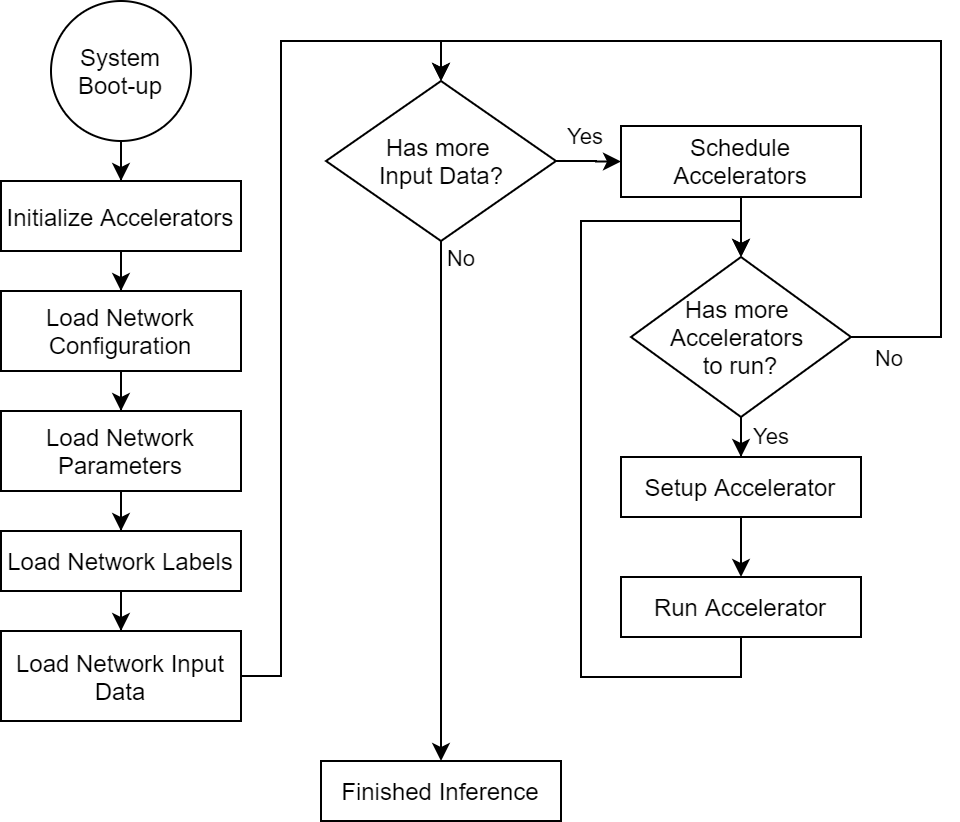
\includegraphics[width=\textwidth]{Images/Platform/PlatformFlowchart.png}
	\decoRule
	\caption[The platform's flowchart]{The platform's flowchart.}
	\label{fig:platform-flowchart}
\end{figure}

\subsection{Scheduler Strategies}
\label{sec:Scheduler-Strategies}
Scheduling can play a significant role in the platform's performance. As mentioned in the previous section, the scheduling strategy is dependent on the platform's implementation and goals. The number of same-type accelerator instances and whether the platform is throughput or latency optimized, all affect the strategy selection. To study and demonstrate the various strategies, a MATLAB model of a CNN network's inference execution was created that can compute the execution characteristics of any CNN network model. This work's main CNN network is AlexNet, on which all experiments below are based.

The MATLAB model creates a timed schedule of a CNN inference depending on its hyperparameters. It computes the number of clock cycles a layer requires for its full execution, and depending on the strategy selected, it places the layer's execution start and finish timestamps. The clock cycles required for every full execution is equal to the sum of the clock cycles needed per assembly instruction to be executed. The number of clock cycles required for every assembly instruction can be set on the MATLAB model's parameters. However, for simplicity, all instructions are considered to run in a single clock cycle.

The following figures show the starting clock cycle, the ending clock cycle, and the duration of every layer, wherever there are colored boxes. Every colored box has its label, defining the layer that it represents. The label is coded as the layer's type and its serial number; Conv for convolutional layers, MaxPool for max-pooling layers, and Linear for fully-connected layers. It should be noted that the ReLU activation function is embedded into the convolutional and fully-connected layers, as shown on algorithms \ref{alg:Convolution-Layer-with-ReLU} and \ref{alg:Fully-Connected-Layer-with-ReLU}.

\subsubsection{Serial Strategy}
A baseline schedule was created using a serial execution strategy, as shown in figure \ref{fig:serial-execution}. In this strategy, every layer starts when the previous layer has finished generating all its outputs. This strategy can be used when there is only one accelerator instance per layer type, and the accelerators do not support layer pipelining. It is also an excellent strategy for debugging and validating the platform and its accelerators because of its simplicity.

\begin{figure} [H]
	\centering
	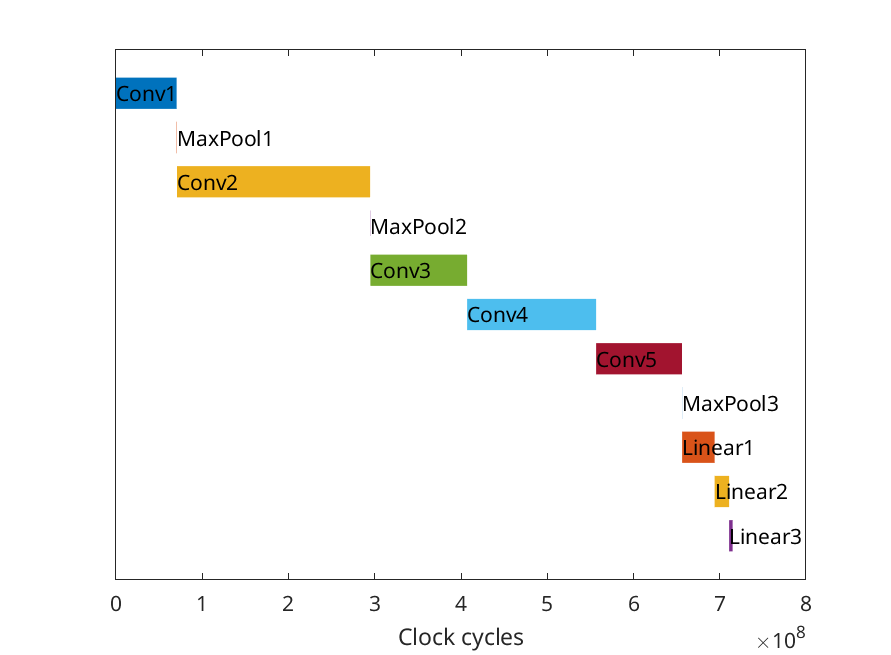
\includegraphics[width=\textwidth]{Images/Scheduling/Serial.png}
	\decoRule
	\caption[AlexNet serial execution]{AlexNet serial execution: Convolution layers consume 90\% of total clock cycles needed for a full inference.}
	\label{fig:serial-execution}
\end{figure}

It can be observed that using the serial execution strategy, around 90\% of the total clock cycles is consumed from the convolutional layers, and almost 0\% is consumed from the max-pooling layers. Hence, according to Amdahl's law, see section \ref{sec:Amdahls-Law}, the convolutional layers should get the most hardware resources for their accelerators to create as much parallelism as possible, while fully-connected layers come next, and max-pooling layers come last.

\subsubsection{Layer-Pipelining Strategy}
Another scheduling strategy is applying pipelining within the layers. In this strategy, a layer is fed with input data as soon as the previous layer generates a single output. This hides the next layer's latency as much as possible by computing outputs in parallel with the computation of its next-to-be-processed inputs. A schedule using the layer-pipelined strategy is shown in figure \ref{fig:layer-pipelined-execution}. To produce such a schedule using this strategy, it is considered to exist as many accelerators per layer type as needed. In this schedule, there are needed five instances of a convolutional accelerator,  three instances of a max-pooling accelerator, and three instances of a fully-connected accelerator.

\begin{figure} [H]
	\centering
	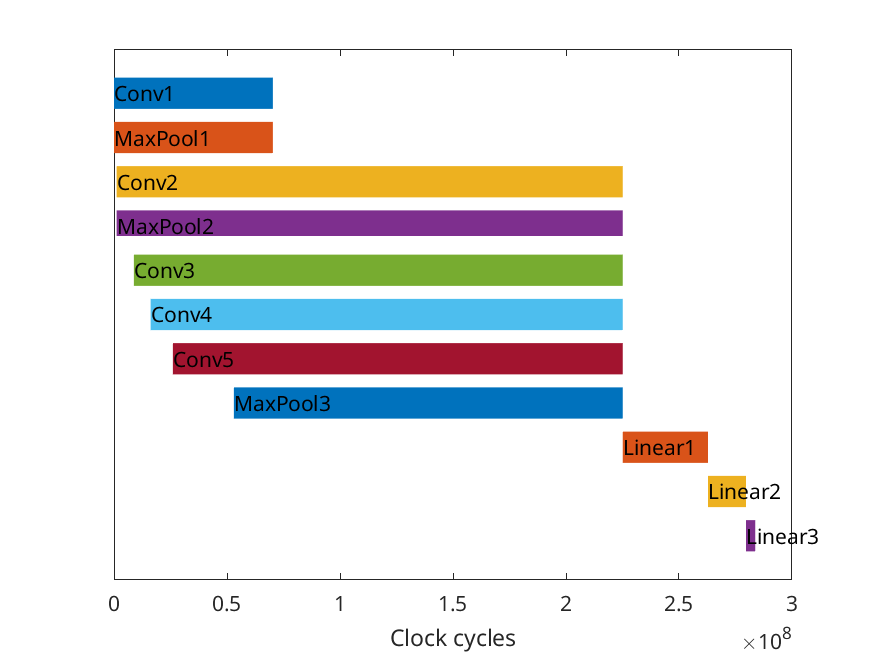
\includegraphics[width=\textwidth]{Images/Scheduling/Pipelined-1x.png}
	\decoRule
	\caption[AlexNet layer-pipelined execution]{AlexNet layer-pipelined execution: There is a speedup of almost 3 times compared to the serial strategy.}
	\label{fig:layer-pipelined-execution}
\end{figure}

The first four layers, Conv1, MaxPool1, Conv2, and MaxPool2 seem to start their execution immediately; however, this is not the case. In fact, they all start on different timestamps, each later from its previous one, but it just cannot be shown in figure \ref{fig:layer-pipelined-execution} due to the x-axis' scale. Conv1, MaxPool1, and Conv2 generate their first outputs in a few clock cycles compared to the x-axis scale. The same artifact appears on the finishing timestamps of the first two layers, Conv1 and MaxPool1, and the next six layers, Conv2 to MaxPool3.

From figure \ref{fig:layer-pipelined-execution}, it can be seen that the whole execution has significantly been reduced compared to the serial strategy shown in figure \ref{fig:serial-execution}, speeding it up almost three times.

However, to use the layer-pipelined strategy, the accelerators have to support it. This means that they need to process their inputs as soon as possible to generate their outputs. Because convolutional and max-pooling layers process their inputs in the 3D and 2D space, they have different implementation requirements to support layer-pipelining, compared to the fully-connected layers that compute their inputs in the 1D space.

Convolutional and max-pooling layers need to process their inputs in a way that they can generate outputs in a specific order. The optimal output order is the one that the next layer wants its inputs to be in, to also produce useful outputs for its next layer. The convolutional and the max-pooling layers produce outputs using cubes or squares of inputs, respectively, starting from the top left input of the grid. Those inputs are created from the previous layer, which also generated them using cubes or squares of inputs. Hence, the deeper the layer, the bigger the required cube or square of the first layer's inputs. Consequently, the optimal order of generating outputs starts from the top left and moving downwards and right in zones, always creating bigger and bigger cubes or squares. Figure \ref{fig:output-generation-order} depicts the order a convolutional or a max-pooling layer generates its outputs. It should be noted that the convolutional layers generate their outputs for all of their output channels, and then they move onto the next output.

\begin{figure} [H]
	\centering
	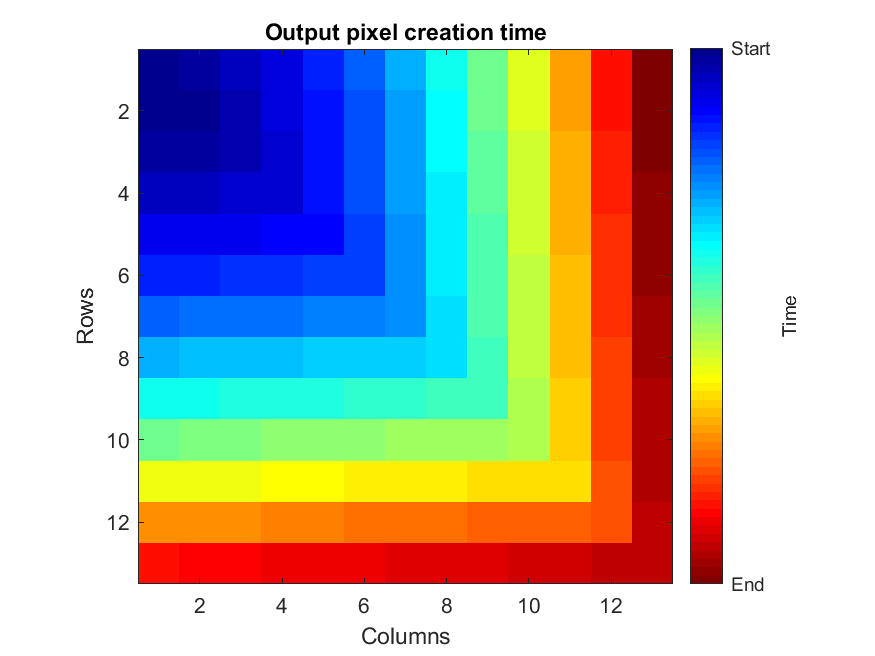
\includegraphics[width=\textwidth]{Images/Scheduling/Conv5-output-creation-time.png}
	\decoRule
	\caption[Convolutional and Max-Pooling layer output order for layer-pipelining]{Convolutional and Max-Pooling layer output order for layer-pipelining: Outputs colored in blue are generated before the red ones.}
	\label{fig:output-generation-order}
\end{figure}

In figure \ref{fig:output-generation-order}, every pixel is an output of a convolutional or max-pooling layer, and it is color-coded concerning the time it is generated, with blue and red colors representing the start and end, respectively, of the generation time.

However, layer-pipelining for convolutional and max-pooling layers significantly increased the implementation complexity of their accelerators. Also, caching weights and inputs in the accelerator's BRAM and registers can become a major obstacle due to their size and access patterns. Figure \ref{fig:Conv5-pixel-frequency} shows the input usage frequency for a convolutional or a max-pooling layer with a stride of one.

\begin{figure} [H]
	\centering
	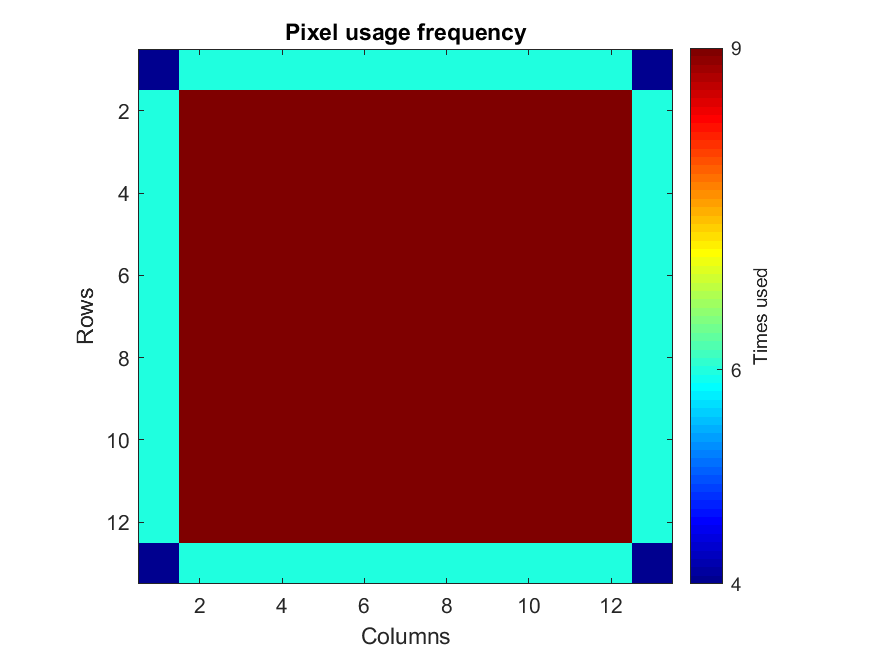
\includegraphics[width=\textwidth]{Images/Scheduling/Conv5-pixel-frequency.png}
	\decoRule
	\caption[Convolutional and Max-Pooling layer input pixel usage frequency using a stride of one]{Convolutional and Max-Pooling layer input pixel usage frequency a stride of one: Blue inputs are rarely used, while red ones are used frequently.}
	\label{fig:Conv5-pixel-frequency}
\end{figure}

Figure \ref{fig:Conv1-pixel-frequency} depicts the input usage frequency for a convolutional or max-pooling layer with a stride of four, showing even more complex access patterns.

\begin{figure} [H]
	\centering
	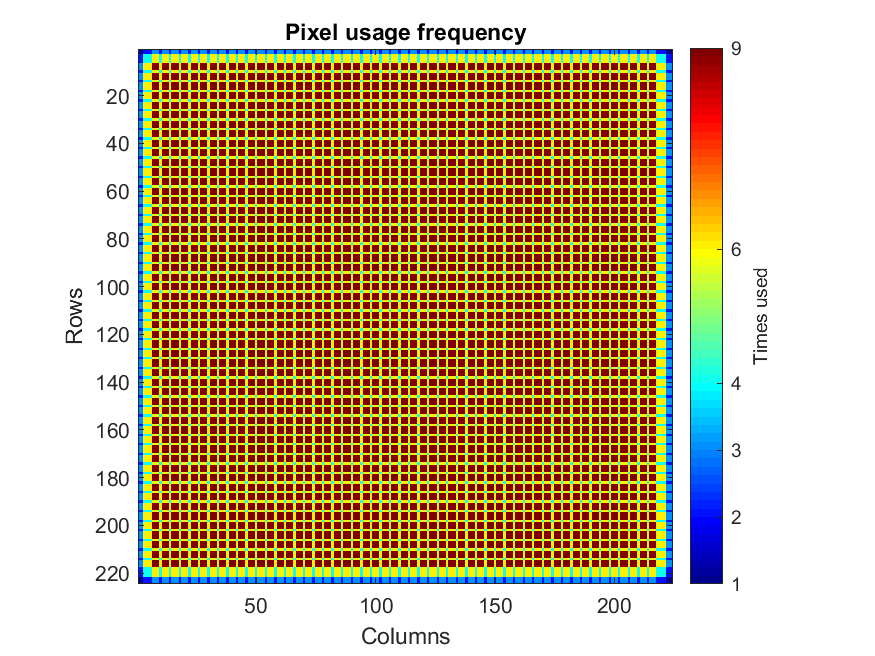
\includegraphics[width=\textwidth]{Images/Scheduling/Conv1-pixel-frequency.png}
	\decoRule
	\caption[Convolutional and Max-Pooling layer input pixel usage frequency using a stride of four]{Convolutional and Max-Pooling layer input pixel usage frequency using a stride of four: Blue inputs are rarely used, while red ones are used frequently.}
	\label{fig:Conv1-pixel-frequency}
\end{figure}

On the other hand, fully-connected layers do not require a specific order for their inputs. However, they need to store partial results for their outputs. Whenever an input is given to the fully-connected layer, it adds it to the partial result of each output after multiplying it with its corresponding weight per output. This creates higher memory requirements for the implementation of the fully-connected accelerator.

Unfortunately, due to the layer-pipelining's significantly increased complexity, this work does not implement it on its accelerators, and it is only presented for completeness and ideas for future work.

\subsubsection{Multi-Inference Strategy}
When multiple accelerators per layer type can be placed into the FPGA device's PL part, they can be utilized simultaneously by running multiple inferences in parallel. The multi-inference strategy schedules two or more images for inference, increasing the platform's overall throughput.

\subsubsection{Image-Pipelining Strategy}
Similar to the multi-inference strategy, when there are multiple accelerators per layer type, multiple images can be fed into the network in a pipelined manner. Every accelerator instance represents a single layer of the network. Hence, the first image can be fed into the first layer. Afterward, when the first layer has generated its outputs, they are fed to the second layer, and the first layer is fed with the second image. This continues for all images to be inferenced. Therefore, when the pipeline is full, all accelerators process different input images from each other. This strategy can decrease the platform's inference latency, and, potentially, the platform's throughput.

\section{Amdahl's Law}
\label{sec:Amdahls-Law}
Amdahl's law \cite{Improvements-in-Multiprocessor-System-Design} is a formula that calculates the theoretical speedup in latency of the execution of a fixed workload task, when the system's resources are improved or increased. While speedup was firstly used on parallel processing, it can also be used after any resource enhancement.

Latency is the time required for a system to compute a single task and is defines as:
\begin{equation}
	\label{eqn:latency}
	\begin{split}
		Latency = \frac{1}{v} = \frac{T}{W},\\
		\mbox{v: the task's execution speed},\\
		\mbox{T: the task's execution time},\\
		\mbox{W: the task's execution workload}\\
	\end{split}
\end{equation}

Throughput is the maximum processing rate of a specific task and is defined as:
\begin{equation}
	\label{eqn:throughput}
	\begin{split}
		Throughput = r * v * A = \frac{r * A * W}{T} = \frac{r * A}{L},\\
		\mbox{r: the execution density},\\
		\mbox{A: the execution capacity}\\
	\end{split}
\end{equation}

The speedup is defined for both latency and throughput, as shown in the equations below:
\begin{equation}
	\label{eqn:latency-speedup}
	\begin{split}
		S_{Latency} = \frac{L_1}{L_2} = \frac{T_1 * W_2}{T_2 * W_1} = \frac{1}{(1 - p) + \frac{p}{s}},\\
		\mbox{p: the task's portion that benefits from the resource enhancements},\\
		\mbox{s: the speedup of the task's portion that benefits from the resource enhancements}\\
	\end{split}
\end{equation}
\begin{equation}
	\label{eqn:throughput-speedup}
	S_{Throughput} = \frac{Throughput_2}{Throughput_1}\\
\end{equation}

The maximum theoretical speedup can also be defined as:
\begin{equation}
	\label{eqn:max-speedup}
	MaxSpeedup = \lim_{s \to \infinity} S_{Latency} = \frac{1}{1 - p}\\
\end{equation}

\section{Platform Accelerator Architectures}
In this work, three different accelerators have been developed, one per layer type used in most CNNs. Those are the convolution, the max-pooling, and the fully-connected accelerators. Every accelerator has two variations; a simple one that only processes a single input similar to serial execution for testing purposes, and a performance-oriented one for production/system deployment. Some of the accelerators' components are being described separately to increase the readability of their architecture diagrams.

\subsection{Convolution Accelerator}
The convolution accelerator is the most complex, requiring lots of BRAM slices and clock cycles to complete. Figure \ref{fig:conv-core-serial} depicts the simple version of the convolution accelerator's architecture. While it is not meant to be used in production, it is great for testing purposes and validating the platform's and accelerator's subsystems.

\begin{figure} [H]
	\centering
	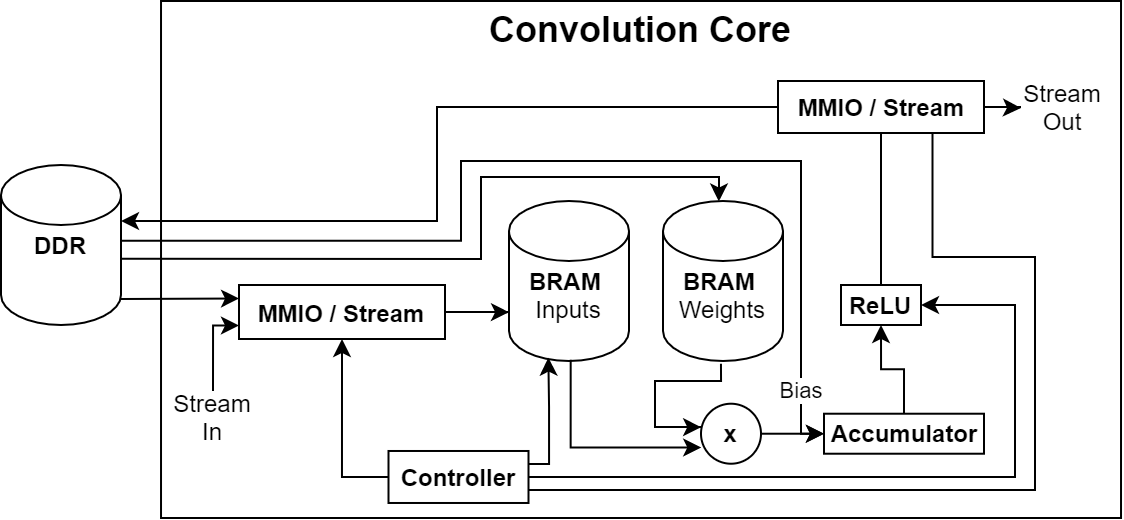
\includegraphics[width=\textwidth]{Images/Platform/Conv_core_serial.png}
	\decoRule
	\caption[Convolutional layer serial accelerator]{Convolutional layer serial accelerator.}
	\label{fig:conv-core-serial}
\end{figure}

The convolution accelerator reaches the platform's DDR memory for its parameters through an AXI4-Full port, while its input data are given either through the same AXI4-Full port or through a dedicated AXI4-Stream port. The input data source is selected using a \emph{MMIO / Stream} component, as instructed by the accelerator's \emph{controller} component, and the data are then stored into a BRAM instance for later use. The layer's weights are stored kernel by kernel onto another BRAM instance. This way, the BRAM requirements are kept low, compared to storing the whole layer's weights, which might also be impossible, due to the BRAM's limited size. Because every kernel is convoluted with the entire input, every weight in that kernel and every input pixel is accessed multiple times. Hence, the inputs and weights BRAM instances are used as caches. It is also worth noting that each BRAM instance implements only one read and one write port because only one input and one weight is accessed every clock cycle.

The computation starts when the input data and weights are stored in their corresponding BRAM instances. Firstly, the \emph{accumulator} component, whose architecture is described below, is initialized by the kernel's bias. Afterward, the controller asks every BRAM instance for specific data to be sent to the \emph{multiplier} component, whose results are then sent to the \emph{accumulator}. This operation continues with the controller selecting the appropriate data for a correct convolution until a single output is ready. Then, it is sent from the \emph{accumulator} to the \emph{ReLU} component, whose architecture is described below. The \emph{controller} then instructs the \emph{ReLU} component to either apply its activation function or pass it through. Lastly, the \emph{ReLU} component sends its output to another \emph{MMIO / Stream} component, which either sends it back to the platform's DDR or a dedicated AXI4-Stream port, also instructed by the \emph{controller}. This procedure continues until the full convolution operation is completed, processing the entire input. The \emph{controller's} configuration is handled by an AXI4-Lite port, accessed by the PS part.

The \emph{accumulator} component, shown in figure \ref{fig:accumulator-component}, is a simple accumulator, which has an input port that gets added with the register's output, used to store the partial result. The adder's output is connected back to the register's input port and the \emph{accumulator} component's output port.

\begin{figure} [H]
	\centering
	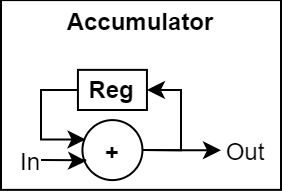
\includegraphics[scale=0.4]{Images/Platform/Accumulator_component.png}
	\decoRule
	\caption[Accumulator component]{Accumulator component.}
	\label{fig:accumulator-component}
\end{figure}

The \emph{ReLU} component, shown in figure \ref{fig:relu-component}, applies the ReLU activation function (see section \ref{sec:Activation-Function}) to the component's input, when the enable port is set, otherwise it passes through the input to the output port. It consists of a simple comparator and two multiplexers.

\begin{figure} [H]
	\centering
	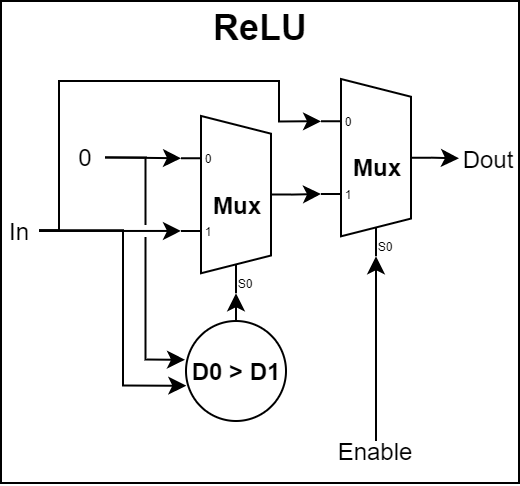
\includegraphics[scale=0.4]{Images/Platform/ReLU_component.png}
	\decoRule
	\caption[ReLU component]{ReLU component.}
	\label{fig:relu-component}
\end{figure}

Figure \ref{fig:conv-core-row-parallel} depicts the high performance version of the convolution accelerator's architecture. It is very similar to the simple version, with the main difference being the number of inputs that can be processed in parallel. This version uses a \emph{multiplier} array, an adder tree, and multiple read and write ports on the input and weights BRAM instances. In this version, the multiplier array is fed with data using all BRAM read ports to feed all of its \emph{multiplier} components in parallel, and then it passes its results to the adder tree in order to create a single partial output. The data fed to the multiplier array consist of a single kernel row of weights and inputs. Then, the partial output is fed to the \emph{accumulator}, and a new row of data is given to the multiplier array. The rows come in the order of top to bottom row of a single channel, and then the next channel follows. This process continues until every row, and channel of a specific kernel is convoluted with the corresponding input area. Afterward, the \emph{accumulator} passes its output to the \emph{ReLU} component, and the process continues similar to the accelerator's simple version.

\begin{figure} [H]
	\centering
	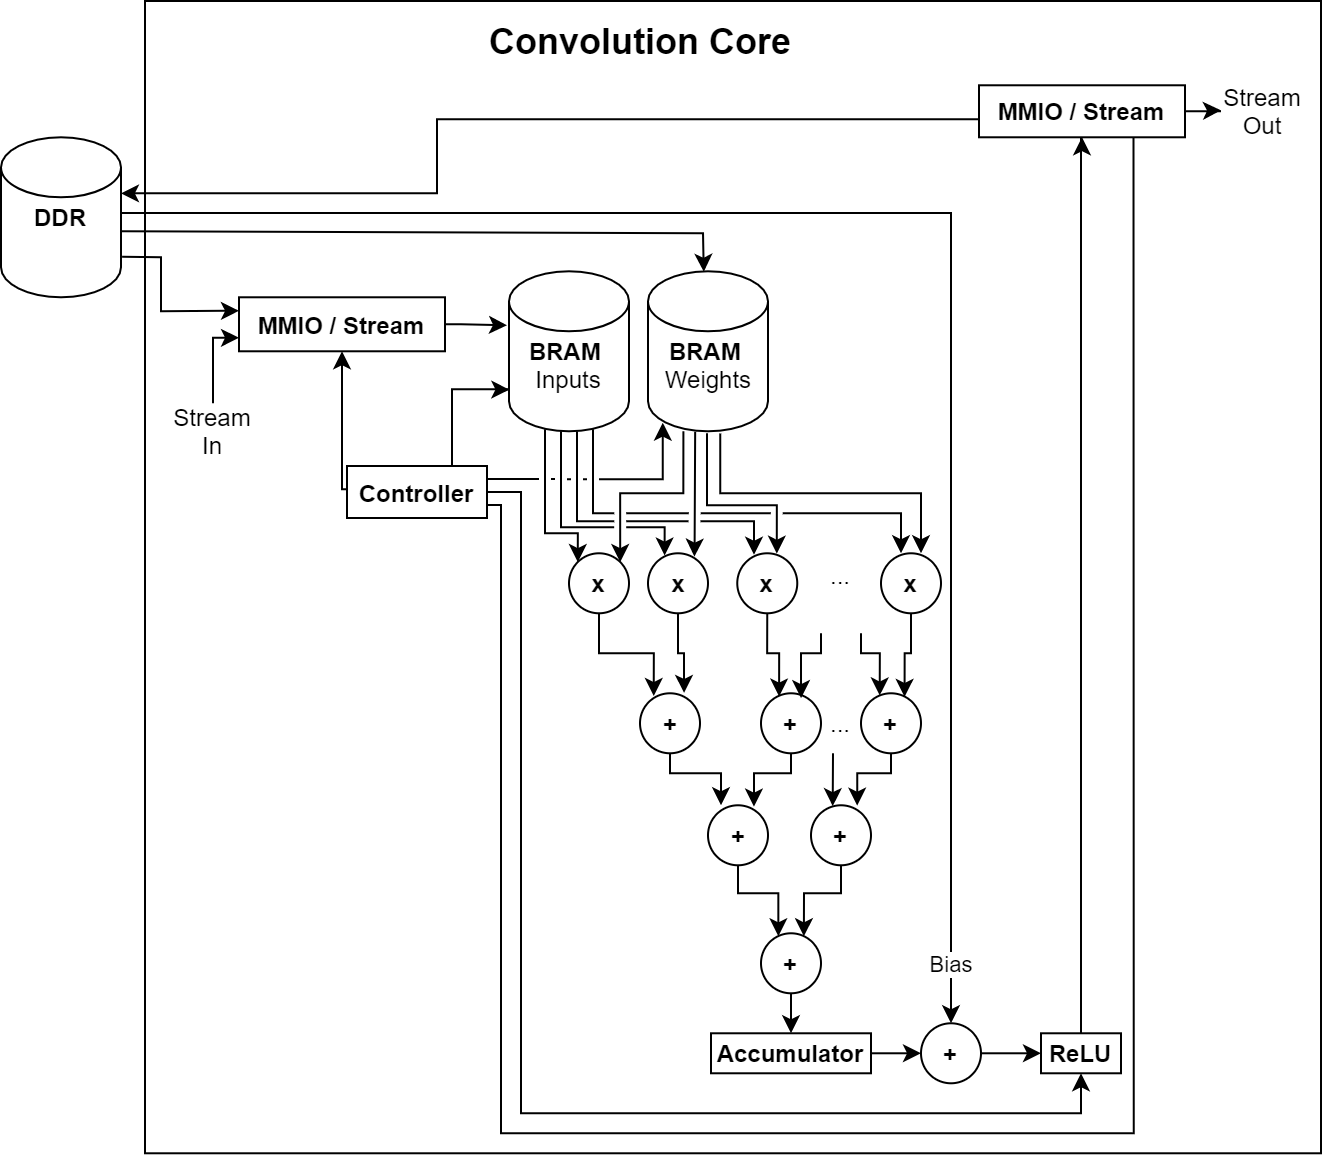
\includegraphics[width=\textwidth]{Images/Platform/Conv_core_row_parallel.png}
	\decoRule
	\caption[Convolutional layer kernel-row-parallel accelerator]{Convolutional layer kernel-row-parallel accelerator.}
	\label{fig:conv-core-row-parallel}
\end{figure}

The number of \emph{multiplier} components is set to be at least the maximum kernel size of every convolutional layer found in the network to be able to process its whole row at once. Granted that the convolution core also has to support the smaller kernel sizes found on the network's convolutional layers, there are structures that feed the excess \emph{multiplier} components with zeros to not affect the computation's result.

\subsection{Max-Pooling Accelerator}
The max-pooling accelerator is the lightest, requiring little BRAM and external I/O. Figure \ref{fig:max-pool-core-serial} depicts the simple version of the accelerator's architecture. Similar to the convolution accelerator, it is not targeted for testing and validation purposes. However, it might also be suitable for production to save resources due to its simplicity. Besides, as shown in the serial scheduling (Figure \ref{fig:serial-execution}), max-pooling layers contribute almost nothing to the overall time required for a complete inference, allowing for slower architectures, saving resources.

\begin{figure} [H]
	\centering
	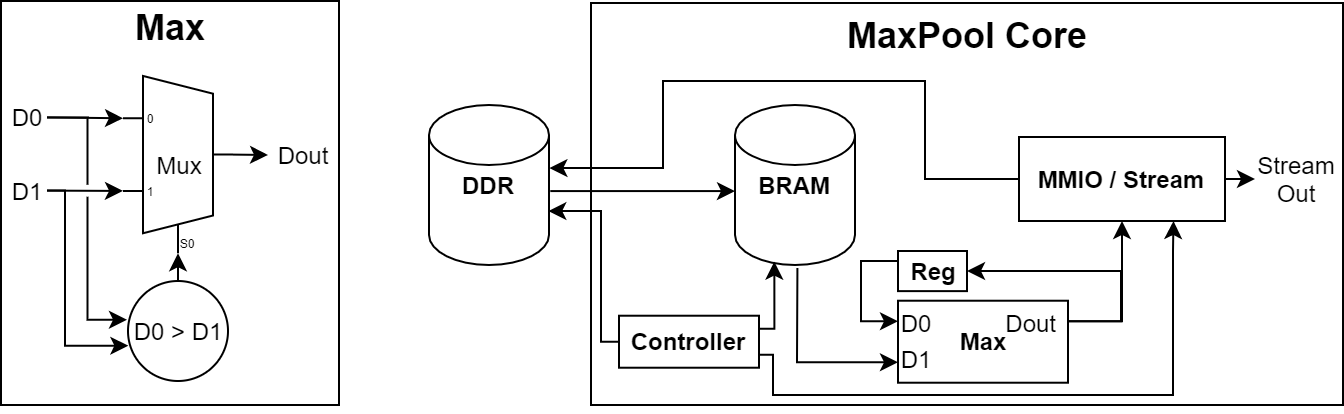
\includegraphics[width=\textwidth]{Images/Platform/MaxPool_core_serial.png}
	\decoRule
	\caption[Max-Pooling layer serial accelerator]{Max-Pooling layer serial accelerator.}
	\label{fig:max-pool-core-serial}
\end{figure}

The max-pooling accelerator's I/O is handled by two \emph{MMIO / Stream} components, similar to the convolutional accelerator. The BRAM instance, using a single read and a single write port, loads a single channel from the whole input. It then feeds the \emph{max} component, whose architecture is described below, as instructed by the accelerator's \emph{controller}. The \emph{max} component's output is fed to the \emph{register}, which feeds it back to the \emph{max} component to process the next input. In other words, this structure finds the maximum value in a given array of input data. This process continues until a whole kernel of input data is processed, generating a single output, which is then sent to the output \emph{MMIO / Stream} component. Afterward, the next part of the input is processed, and when the whole channel is completed, the next one gets loaded to the BRAM instance. The accelerator finishes when all of the input channels are processed.

The \emph{max} component, shown in figure \ref{fig:max-component}, outputs the maximum input of the two it is given. It comprises only two components, a comparator, and a multiplexer.

\begin{figure} [H]
	\centering
	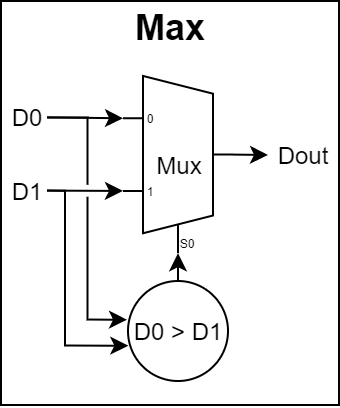
\includegraphics[scale=0.4]{Images/Platform/Max_component.png}
	\decoRule
	\caption[Max component]{Max component.}
	\label{fig:max-component}
\end{figure}

The max-pooling accelerator's high performance version architecture is depicted in figure \ref{fig:max-pool-core-kernel-parallel}. The difference between the simple architecture lies upon the BRAM instance's read ports number and the \emph{max tree} component, whose architecture is described below. Using multiple read ports, multiple inputs can be inserted to the \emph{max tree} component in a single clock cycle, which in turn it outputs the max value of its given input. This architecture processes the whole kernel, generating a single output in every iteration. On every iteration, the kernel moves onto the given input, until the channel is fully processed. Then the next channel gets loaded onto the BRAM instance, and the process continues.

\begin{figure} [H]
	\centering
	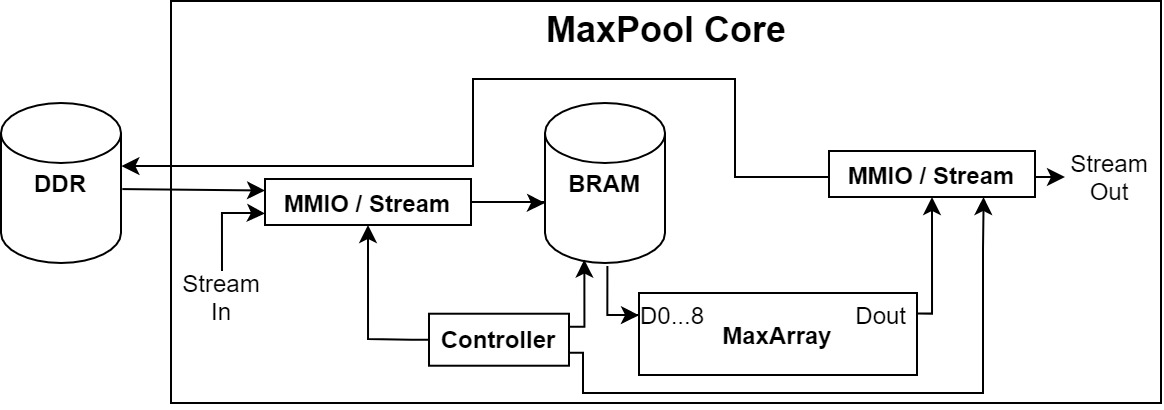
\includegraphics[width=\textwidth]{Images/Platform/MaxPool_core_kernel_parallel.png}
	\decoRule
	\caption[Max-Pooling layer kernel-parallel accelerator]{Max-Pooling layer kernel-parallel accelerator.}
	\label{fig:max-pool-core-kernel-parallel}
\end{figure}

Like the convolution accelerator, the max-pooling accelerator must support all kernel sizes found in the network's max-pooling layer. Hence, the BRAM read ports number and the \emph{max tree} component's input ports number are set to be the network's maximum max-pooling kernel size. When a layer with a smaller kernel size is processed, the \emph{max tree} component's excess inputs are fed with the minimum possible value not to affect the computation.

The \emph{max tree} component, shown in figure \ref{fig:max-tree-component}, is a tree of \emph{max} components, capable of finding the max value from the given input. The kernel's 2D matrix is flattened into a 1D array fed into the \emph{max tree} component to find the input area's maximum value.

\begin{figure} [H]
	\centering
	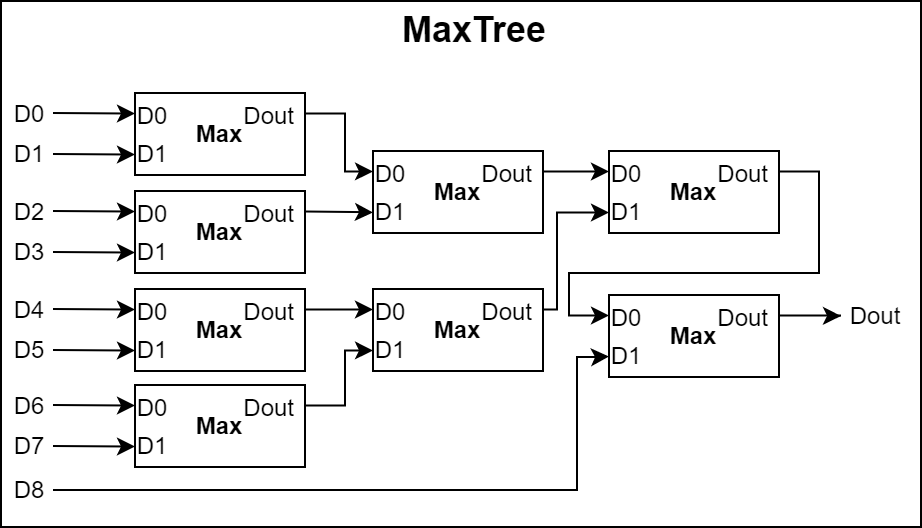
\includegraphics[width=\textwidth]{Images/Platform/MaxTree_component.png}
	\decoRule
	\caption[MaxTree component]{MaxTree component.}
	\label{fig:max-tree-component}
\end{figure}

\subsection{Fully-Connected Accelerator}
Unfortunately, the fully-connected accelerator is the most limited in terms of parallelism capabilities since the fully-connected layer's weights are used only once, and therefore, they cannot be cached into an in-accelerator memory instance (BRAM or registers). Only the input data are used multiple times, so storing them into a BRAM instance can help avoid I/O with the platform's DDR.

Figure \ref{fig:linear-core-serial} shows the simple version of the fully-connected accelerator's architecture. Like the other accelerators, the input and output data are handled, as instructed by the accelerator's \emph{controller}, using two \emph{MMIO / Stream} components, connected to their dedicated input and output AXI4-Stream ports and the AXI4-Full port. Firstly, the input data are loaded onto the BRAM instance, through the input \emph{MMIO / Stream} component. Afterward, the \emph{accumulator} component is initialized with the appropriate bias, read directly from the platform's DDR through the accelerator's AXI4-Full port. Then, the \emph{controller} instructs the BRAM instance to sequentially fed the \emph{multiplier} with a single input datum on every iteration. It also instructs the DDR to feed the \emph{multiplier}, through the AXI4-Full port, with the corresponding weight on every iteration. The \emph{multiplier} component's output is then forwarded to the \emph{accumulator}. When all weights and inputs are multiplied and accumulated, a single output is generated. It is then sent from the \emph{accumulator} directly to the \emph{ReLU} component, which applies its ReLU activation function if instructed so by the \emph{controller}. Lastly, the \emph{ReLU} component's result is sent to the output \emph{MMIO / Stream} component to write it back to the DDR or to send it to the next accelerator using its dedicated output stream port. The accelerator finishes when all inputs and all weights have been processed, generating the total output.

\begin{figure} [H]
	\centering
	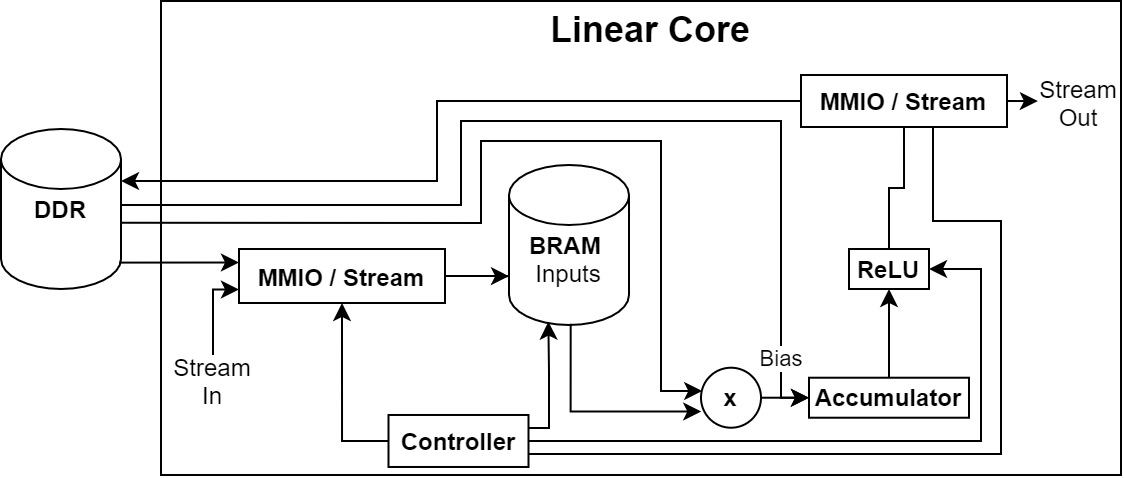
\includegraphics[width=\textwidth]{Images/Platform/Linear_core_serial.png}
	\decoRule
	\caption[Fully-Connected layer serial accelerator]{Fully-Connected layer serial accelerator.}
	\label{fig:linear-core-serial}
\end{figure}

Although this version is relatively simple, it uses a lot of BRAM only to access a single input, sequentially. Hence, the BRAM instance might be overkill for this use, wasting resources. Although, it should be noted that this simple version of the accelerator's architecture is only targeted for testing and validation purposes.

A more optimized architecture can be seen in figure \ref{fig:linear-core-partial-outputs}, where a multiplier array and an adder tree are utilized, the input BRAM instance is replaced with simple registers, and the weights are given by splitting the 128-bit wide AXI4-Full port. In a sense, the accelerator processes its input data in parts creating partial outputs on each iteration.

\begin{figure} [H]
	\centering
	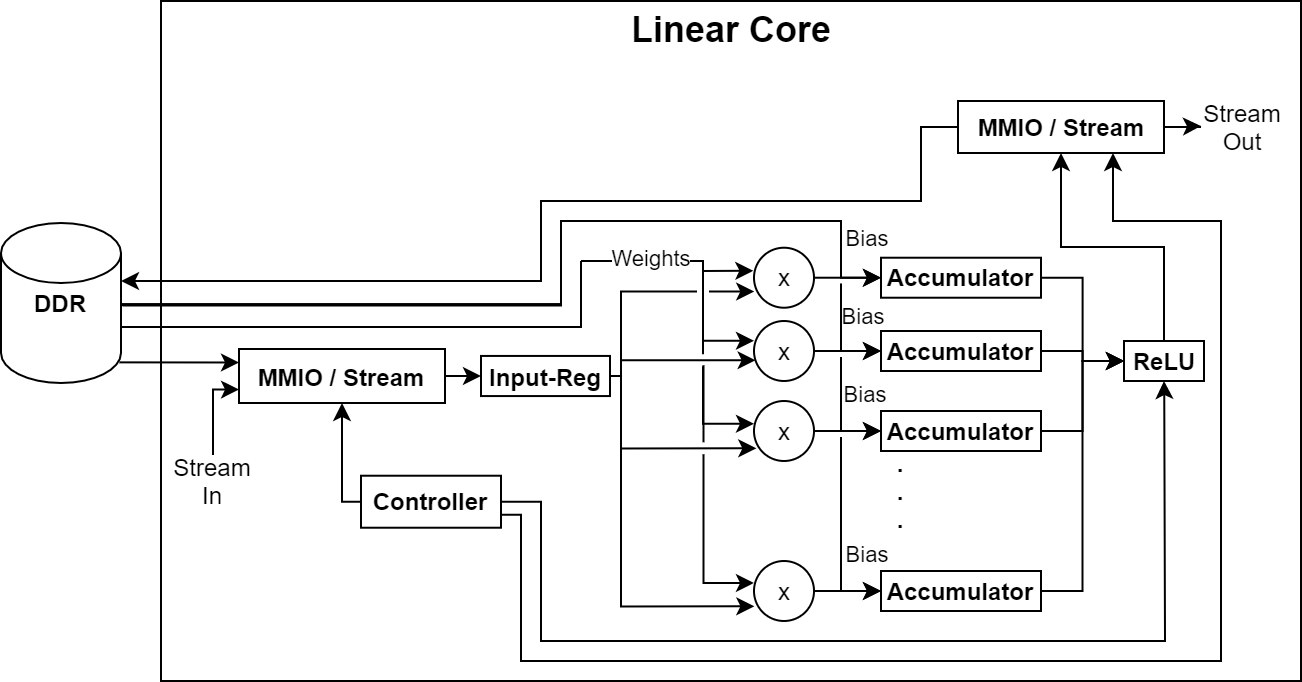
\includegraphics[width=\textwidth]{Images/Platform/Linear_core_partial_outputs.png}
	\decoRule
	\caption[Fully-Connected layer accelerator with partial outputs]{Fully-Connected layer accelerator with partial outputs.}
	\label{fig:linear-core-partial-outputs}
\end{figure}

Like the simple version, the input data are handled by the input \emph{MMIO / Stream} component; however, they are then written in parts onto the \emph{input registers}. Every register has its own read and write ports so that multiple inputs can be sent to the multiplier array in parallel. Furthermore, the weights are still read from the DDR through the accelerator's AXI4-Full port, taking advantage of the port's width. For example, if a single weight is a 32-bit float and the port is 128-bit wide, every 128-bit word can include four weights. Hence, the size of the multiplier array depends on the weight's data type. Also, there is no need for more input registers than the number of weights that can fit into a single 128-bit word, so the input data are saved and processed in parts throughout the whole output. The process starts by initializing the output BRAM instance with the biases. The output BRAM instance is used to store the partial outputs; therefore, every cell is initialized with a single bias, corresponding to the output it represents. Starting the computation, the first input part is multiplied with its corresponding weights, and then the multiplication's results are sent to the added tree, generating a partial output stored into its BRAM cell. Afterward, the same input part is multiplied with the next set of weights, and a new partial output is generated and stored. When the first input part has been processed throughout all the partial outputs, the second part takes its place, and the process continues, adding the newly created partial outputs to the already existing ones in the BRAM's cells. The process continues until the whole input has been processed, and the full outputs are generated. Lastly, the full outputs pass through the \emph{ReLU} component and are then sent to the \emph{MMIO / Stream} component.

\chapter{Results}
This work's implementation of the proposed platform is described in section \ref{sec:proposed-platform-implementation}. Its performance metrics, such as its latency, throughput, power, and energy consumption, are compared to the available alternative technologies and FPGA architectures. AlexNet is the selected CNN to be used as a benchmark for the various technologies compared.

\section{Specifications of the Compared Platforms}
The proposed platform is compared with an Intel i7 4710MQ CPU, an NVIDIA RTX 2060 Super 8GB GPU, a Xilinx CHaiDNN implementation, and a Xilinx DPU implementation. All FPGA implementations, including this work's platform, use the Xilinx ZCU102 Evaluation board.

% \subsection{AMD Ryzen 5 1400}
% The AMD Ryzen 5 1400 CPU \cite{AMD-Ryzen-5-1400-Processor}, released in 2017, is a desktop processor targeted for mid-range productivity computers. Its specifications are presented in table \ref{tab:AMD-Ryzen-5-1400-specs}.

% \begin{table}[H]
% 	\caption{AMD Ryzen 5 1400 processor specifications}
% 	\label{tab:AMD-Ryzen-5-1400-specs}
% 	\centering
% 	\begin{tabular}{ll}
% 		\toprule
% 		\textbf{Cores / Threads} & 4/8\\
% 		\textbf{Max Turbo Frequency} & 3.4GHz\\
% 		\textbf{TDP} & 65W\\
% 		\textbf{Max Memory Bandwidth} & 42.7GB/s\\
% 		\textbf{Lithography} & 14nm\\
% 		\bottomrule\\
% 	\end{tabular}
% \end{table}

\subsection{Intel i7 4710MQ}
The Intel i7 4710MQ CPU \cite{Intel-i7-4710MQ-Processor}, released in 2014, is a mobile processor targeted for high-performance laptops. Its specifications are presented in table \ref{tab:Intel-i7-4710MQ-specs}.

\begin{table}[H]
	\caption{Intel i7 4710MQ processor specifications}
	\label{tab:Intel-i7-4710MQ-specs}
	\centering
	\begin{tabular}{ll}
		\toprule
		\textbf{Cores / Threads} & 4/8\\
		\textbf{Max Turbo Frequency} & 3.5GHz\\
		\textbf{TDP} & 47W\\
		\textbf{Max Memory Bandwidth} & 25.6GB/s\\
		\textbf{Lithography} & 22nm\\
		\bottomrule\\
	\end{tabular}
\end{table}

\subsection{NVIDIA RTX-2060 Super 8GB}
The NVIDIA RTX-2060 Super \cite{NVIDIA-RTX-2060-Super}, released in 2019, is a desktop GPU, and while targeted for raytraced gaming, it is also suitable for CNN inferencing due to its large and high-bandwidth memory. Its specifications are presented in table \ref{tab:NVIDIA-RTX-2060-Super-specs}.

\begin{table}[H]
	\caption{NVIDIA RTX 2060 Super specifications}
	\label{tab:NVIDIA-RTX-2060-Super-specs}
	\centering
	\begin{tabular}{ll}
		\toprule
		\textbf{CUDA Cores} & 2176\\
		\textbf{GPU Memory} & 8GB GDDR6\\
		\textbf{Boost Clock} & 1650 MHz\\
		\textbf{Memory Interface} & 256-bit\\
		\textbf{Memory Bandwidth} & 448GB/s\\
		\textbf{Power Consumption} & 175W\\
		\bottomrule\\
	\end{tabular}
\end{table}

\subsection{Xilinx CHaiDNN}
The Xilinx CHaiDNN accelerator library, presented in section \ref{sec:Xilinx-CHaiDNN}, was implemented for this work's comparisons. The resource utilization for its implementation is depicted in table \ref{tab:CHaiDNN-resource-usage}. It should be noted that Double Pumped DSPs are used.

\begin{table}[H]
	\caption{Xilinx CHaiDNN resource usage}
	\label{tab:CHaiDNN-resource-usage}
	\centering
	\begin{tabular}{ll}
		\toprule
		\textbf{PL/DSP Clock Frequency} & 250/500 MHz\\
		\textbf{LUT Usage} & 59.1\%\\
		\textbf{LUTRAM Usage} & -\\
		\textbf{FF Usage} & 27.66\%\\
		\textbf{BRAM Usage} & 74.12\%\\
		\textbf{DSP Usage} & 53.65\%\\
		\textbf{BUFG Usage} & -\\
		\bottomrule\\
	\end{tabular}
\end{table}

% \subsection{Xilinx DPU}
% The Xilinx DPU accelerator library, presented in section \ref{sec:Xilinx-DPU}, was implemented for this work's comparisons. The resource utilization for its implementation is depicted in table \ref{tab:DPU-resource-usage}.

% \begin{table}[H]
% 	\caption{Xilinx DPU resource usage}
% 	\label{tab:DPU-resource-usage}
% 	\centering
% 	\begin{tabular}{ll}
% 		\toprule
% 		\textbf{Clock Frequency (MHz)} & 300/600\\
% 		\textbf{LUT Usage (\%)} & 7.34\\
% 		\textbf{LUTRAM Usage (\%)} & 2.05\\
% 		\textbf{FF Usage (\%)} & 4.03\\
% 		\textbf{BRAM Usage (\%)} & 7.51\\
% 		\textbf{DSP Usage (\%)} & 1.9\\
% 		\textbf{BUFG (\%)} & 0.25\\
% 		\bottomrule\\
% 	\end{tabular}
% \end{table}

\section{Proposed Platform}
\label{sec:proposed-platform-implementation}
This work's proposed platform can be implemented using several data types and accelerators. For this comparison, it was implemented based on AlexNet's requirements and characteristics, presented in chapter \ref{Chapter-Theoretical-Modeling-and-Robustness-Analysis}. Both parameters and activations are represented as 8-bit fixed-points; hence, the accelerators use the same data type. There is a single accelerator instance per layer type, using their high-performance versions as presented in section \ref{sec:Platform-Accelerator-Architectures}. The serial execution scheduler (see section \ref{sec:Scheduler-Strategies}) was selected because the implemented accelerators do not support layer pipelining, and there are not multiple instances per layer type.

The resource utilization for implementing the aforementioned configuration of the proposed platform is depicted in table \ref{tab:Proposed-platform-resource-usage}.

\begin{table}[H]
	\caption{Proposed platform resource usage}
	\label{tab:Proposed-platform-resource-usage}
	\centering
	\begin{tabular}{ll}
		\toprule
		\textbf{Clock Frequency (MHz)} & 300MHz\\
		\textbf{LUT Usage} & 7.34\%\\
		\textbf{LUTRAM Usage} & 2.05\%\\
		\textbf{FF Usage} & 4.03\%\\
		\textbf{BRAM Usage} & 7.51\%\\
		\textbf{DSP Usage} & 1.9\%\\
		\textbf{BUFG (\%)} & 0.25\%\\
		\bottomrule\\
	\end{tabular}
\end{table}

\section{Power Consumption}
Power consumption is defined as the energy consumed per unit time for accomplishing a specific task, from a chemical reaction and lifting materials using a crane, to emitting light through a light bulb and inferencing CNNs on electronic hardware. Average power consumption is always preferred to be as low as possible to increase the system's energy efficiency, minimizing energy losses. In addition, low power consumption leads to simpler system designs and lower building costs. It is usually measured in Watts (w) or kiloWatts (kW).

\section{Energy Consumption}
Energy consumption is defined as the energy required for accomplishing a specific task in a specific time amount. It can be calculated as $Energy = Power * Time$, where $Power$ is the required power, and $Time$ is the required time for accomplishing the task. Energy consumption is also preferred to be as low as possible while accomplishing the given task within the time constraints, to minimize the operational costs. It is usually measured in Joule (J) or kiloJoule (kJ).

\section{Throughput and Latency}
Throughput, defined in equation \ref{eqn:throughput}, is the number of tasks that can be accomplished in a unit time. It is preferred to be as high as possible to generate as much work as possible in the unit time.

Latency, defined in equation \ref{eqn:latency}, is the time required for accomplishing a single task. It is preferred to be as low as possible to finish tasks as quickly as possible from the time they are issued.



\section{Final Performance}
The comparisons were conducted using the same dataset and AlexNet hyper-parameters across all technologies. The CPU and GPU use floating-point arithmetic for their parameters and activations, while CHaiDNN uses 6-bit quantization, and the proposed platform implementation, TUCNNPU, uses 8-bit fixed-point arithmetic.

Table \ref{tab:Performance-results} depicts the comparison results of every technology.

\begin{table}[H]
	\caption{Performance results}
	\label{tab:Performance-results}
	\centering
	\begin{tabular}{lllll}
		\toprule
		& \textbf{CPU} & \textbf{GPU} & \textbf{CHaiDNN} & \textbf{TUCNNPU}\\
		\midrule
			\textbf{Clock Frequency (MHz)} & 3500 & 1650 & 250/500 & 300\\
			\textbf{Throughput (Images/s)} & 94.84 & 5784.6 & 10.07 & 0.0927\\
			\textbf{Throughput Speedup} & 1.0000x & 60.9933x & 0.1062x & 0.0010x\\
			\textbf{Latency (s)} & 0.0266 & 0.0009 & 0.0993 & 10.783\\
			\textbf{Latency Speedup} & 1.0000x & 29.5556x & 0.2679x & 0.0025x\\
			\textbf{Total On-Chip Power (Watt)} & 47 & 175 & 19.3 & 4.559\\
			\textbf{Power Efficiency} & 1.0000x & 0.2686x & 2.4352x & 10.3093x\\
			\textbf{Energy Cons./Image (Joule)} & 1.2502 & 0.1575 & 1.9165 & 49.1597\\
			\textbf{Energy Efficiency} & 1.0000x & 7.9378x & 0.6523x & 0.0254x\\
			\textbf{Images/Joule} & 2.0179 & 33.0549 & 0.5218 & 0.0203\\
		\bottomrule\\
	\end{tabular}
\end{table}

\chapter{Conclusions and Future Work}
\label{Chapter-Conclusions-and-Future-Work}
In this chapter, this thesis' work is being summed up and evaluated. Also, directions for future work, possible extensions, and optimizations are being given.

\section{Conclusions}
Over the last few years, Convolutional Neural Networks have proved to be capable of tackling complex image recognition problems and sound recognition, security, and data mining problems. The research community continues to surprise the world with new and paradoxical use cases for CNNs, with even more exciting results. With the rise of neural networks, hardware capable of handling high computational complexity in a fast and energy-efficient manner becomes necessary.

This thesis' purpose was to create an FPGA accelerator for CNN inference, using AlexNet as the base network and benchmark. However, a whole platform was created for easy and structured implementation of such accelerators not only for CNNs but neural networks in general. The implementation of this thesis' proposed platform is used to accelerate AlexNet's inference, whose robustness analysis was carried out to investigate the FPGA's strengths and weaknesses. Computational workloads, memory access patterns, memory and bandwidth reduction, as well as algorithmic optimizations, were studied to exploit the FPGA's parallelism capabilities and strengths.

% Todo: Fill speedup results
While the proposed platform's implementation was based on the Xilinx ZCU102 Evaluation Kit, it can be transferred and scaled accordingly to other FPGA devices, such as the FORTH QFDB, a custom four-FPGA platform. The implemented platform managed to achieve a x latency speedup, a x throughput speedup, while retaining a x energy efficiency over an NVIDIA RTX-2060 Super GPU.

\section{Future Work}
This thesis' proposed platform is by design easily expandable for future use and development, creating several opportunities for its expansion and CNN accelerators' optimization. Some of them are presented below.
\begin{itemize}
	\item Quantization techniques for both parameters and activations should be further investigated to achieve better classification accuracy using 8-bit or even lower representations. Techniques such as K-Means clustering, Lloyd's, Pair and Quad compression, and SLC found in George Pitsis' thesis \cite{Design-and-implementation-of-an-FPGA-based-convolutional-neural-network-accelerator} could be a great start.
	\item Similar to integrating the ReLU activation function into the Convolutional and Fully-Connected layers' accelerators, integrating the pooling layer into the convolutional layer's accelerator could be beneficial both latency and throughput by reducing the network's overall memory I/O and avoiding the separate accelerator's initialization.
	\item The platform's scalability should be exploited not only by implementing it in bigger FPGA devices but also in multiple interconnected FPGAs using platforms such as the FORTH QFDB or CRDB. Multiple accelerator instances could be incorporated using such platforms, creating opportunities for higher throughput and lower latency, as well as new scheduler strategies that might not be presented in the FPGA Implementation chapter.
	\item Pruning enabled accelerators could bring not only lower latency and high throughput but also higher energy efficiency since there are less required operations for a single inference.
	\item There are works, such as the Xilinx DPU, which use systolic arrays as their main compute engine. Systolic arrays, while being relatively complicated, could improve latency and memory bandwidth due to their design. They could be used to implement a matrix multiplier for the convolutional layer's operation requirements. Although implementing variable padding and stride is not an obvious task, it should be feasible with careful data scheduling. Also, systolic arrays could be designed to implement n-dimensional convolutions to expand the accelerator's use cases.
	\item Monte Carlo Dropout during inference could also be consolidated to increase the confidence of the classification results. Multiple instances of the same network could be run with the same inputs in parallel, using multiple accelerator instances and even multiple FPGA devices. Weight could be zeroed out randomly on each iteration in hardware using a linear feedback shift register as a random number generator.
	\item Layer-Pipelining, as presented in section \ref{sec:Scheduler-Strategies}, could further decrease the network's overall latency. While implementing it as presented is a complex task, it could be simplified by implementing a memory address generator that produces addresses in the specified order.
	\item During some experimentation with Xilinx's tools, it was observed that implementing the same functionality designs using pure VHDL and Xilinx HLS leads to very different performance and especially resource utilization. Although implementing a design using pure VHDL requires much more working hours on its development and testing compared to using Xilinx HLS, it could create better performance results and new opportunities.
	\item CPU-FPGA partitioning should also be further studied to exploit the CPU's higher clock speeds, avoiding wasting FPGA resources for tasks that CPUs can already handle. In the case of Xilinx ZCU102, all six cores could be utilized to contribute to the overall network inference.
\end{itemize}


%----------------------------------------------------------------------------------------
%	THESIS CONTENT - APPENDICES
%----------------------------------------------------------------------------------------

\appendix % Cue to tell LaTeX that the following "chapters" are Appendices

% Include the appendices of the thesis as separate files from the Appendices folder
% Uncomment the lines as you write the Appendices

% % Appendix A

\chapter{Frequently Asked Questions} % Main appendix title

\label{AppendixA} % For referencing this appendix elsewhere, use \ref{AppendixA}

\section{How do I change the colors of links?}

The color of links can be changed to your liking using:

{\small\verb!\hypersetup{urlcolor=red}!}, or

{\small\verb!\hypersetup{citecolor=green}!}, or

{\small\verb!\hypersetup{allcolor=blue}!}.

\noindent If you want to completely hide the links, you can use:

{\small\verb!\hypersetup{allcolors=.}!}, or even better: 

{\small\verb!\hypersetup{hidelinks}!}.

\noindent If you want to have obvious links in the PDF but not the printed text, use:

{\small\verb!\hypersetup{colorlinks=false}!}.

% \include{Appendices/AppendixB}
% \include{Appendices/AppendixC}

%----------------------------------------------------------------------------------------
%	BIBLIOGRAPHY
%----------------------------------------------------------------------------------------

% \printbibliography[heading=bibintoc]

\cleardoublepage
\phantomsection
\addcontentsline{toc}{chapter}{References}
\printbibliography[keyword={References}, title={References}]
\printbibliography[keyword={Link}, title={External Links}]

%----------------------------------------------------------------------------------------

\end{document}
